\documentclass[twoside]{book}

% Packages required by doxygen
\usepackage{fixltx2e}
\usepackage{calc}
\usepackage{doxygen}
\usepackage[export]{adjustbox} % also loads graphicx
\usepackage{graphicx}
\usepackage[utf8]{inputenc}
\usepackage{makeidx}
\usepackage{multicol}
\usepackage{multirow}
\PassOptionsToPackage{warn}{textcomp}
\usepackage{textcomp}
\usepackage[nointegrals]{wasysym}
\usepackage[table]{xcolor}

% Font selection
\usepackage[T1]{fontenc}
\usepackage[scaled=.90]{helvet}
\usepackage{courier}
\usepackage{amssymb}
\usepackage{sectsty}
\renewcommand{\familydefault}{\sfdefault}
\allsectionsfont{%
  \fontseries{bc}\selectfont%
  \color{darkgray}%
}
\renewcommand{\DoxyLabelFont}{%
  \fontseries{bc}\selectfont%
  \color{darkgray}%
}
\newcommand{\+}{\discretionary{\mbox{\scriptsize$\hookleftarrow$}}{}{}}

% Page & text layout
\usepackage{geometry}
\geometry{%
  a4paper,%
  top=2.5cm,%
  bottom=2.5cm,%
  left=2.5cm,%
  right=2.5cm%
}
\tolerance=750
\hfuzz=15pt
\hbadness=750
\setlength{\emergencystretch}{15pt}
\setlength{\parindent}{0cm}
\setlength{\parskip}{3ex plus 2ex minus 2ex}
\makeatletter
\renewcommand{\paragraph}{%
  \@startsection{paragraph}{4}{0ex}{-1.0ex}{1.0ex}{%
    \normalfont\normalsize\bfseries\SS@parafont%
  }%
}
\renewcommand{\subparagraph}{%
  \@startsection{subparagraph}{5}{0ex}{-1.0ex}{1.0ex}{%
    \normalfont\normalsize\bfseries\SS@subparafont%
  }%
}
\makeatother

% Headers & footers
\usepackage{fancyhdr}
\pagestyle{fancyplain}
\fancyhead[LE]{\fancyplain{}{\bfseries\thepage}}
\fancyhead[CE]{\fancyplain{}{}}
\fancyhead[RE]{\fancyplain{}{\bfseries\leftmark}}
\fancyhead[LO]{\fancyplain{}{\bfseries\rightmark}}
\fancyhead[CO]{\fancyplain{}{}}
\fancyhead[RO]{\fancyplain{}{\bfseries\thepage}}
\fancyfoot[LE]{\fancyplain{}{}}
\fancyfoot[CE]{\fancyplain{}{}}
\fancyfoot[RE]{\fancyplain{}{\bfseries\scriptsize Generated by Doxygen }}
\fancyfoot[LO]{\fancyplain{}{\bfseries\scriptsize Generated by Doxygen }}
\fancyfoot[CO]{\fancyplain{}{}}
\fancyfoot[RO]{\fancyplain{}{}}
\renewcommand{\footrulewidth}{0.4pt}
\renewcommand{\chaptermark}[1]{%
  \markboth{#1}{}%
}
\renewcommand{\sectionmark}[1]{%
  \markright{\thesection\ #1}%
}

% Indices & bibliography
\usepackage{natbib}
\usepackage[titles]{tocloft}
\setcounter{tocdepth}{3}
\setcounter{secnumdepth}{5}
\makeindex

% Hyperlinks (required, but should be loaded last)
\usepackage{ifpdf}
\ifpdf
  \usepackage[pdftex,pagebackref=true]{hyperref}
\else
  \usepackage[ps2pdf,pagebackref=true]{hyperref}
\fi
\hypersetup{%
  colorlinks=true,%
  linkcolor=blue,%
  citecolor=blue,%
  unicode%
}

% Custom commands
\newcommand{\clearemptydoublepage}{%
  \newpage{\pagestyle{empty}\cleardoublepage}%
}

\usepackage{caption}
\captionsetup{labelsep=space,justification=centering,font={bf},singlelinecheck=off,skip=4pt,position=top}

%===== C O N T E N T S =====

\begin{document}

% Titlepage & ToC
\hypersetup{pageanchor=false,
             bookmarksnumbered=true,
             pdfencoding=unicode
            }
\pagenumbering{alph}
\begin{titlepage}
\vspace*{7cm}
\begin{center}%
{\Large My Project }\\
\vspace*{1cm}
{\large Generated by Doxygen 1.8.13}\\
\end{center}
\end{titlepage}
\clearemptydoublepage
\pagenumbering{roman}
\tableofcontents
\clearemptydoublepage
\pagenumbering{arabic}
\hypersetup{pageanchor=true}

%--- Begin generated contents ---
\chapter{Namespace Index}
\section{Namespace List}
Here is a list of all documented namespaces with brief descriptions\+:\begin{DoxyCompactList}
\item\contentsline{section}{\hyperlink{namespaceimage__tools}{image\+\_\+tools} \\*\+:sfjsklkj }{\pageref{namespaceimage__tools}}{}
\end{DoxyCompactList}

\chapter{Hierarchical Index}
\section{Class Hierarchy}
This inheritance list is sorted roughly, but not completely, alphabetically\+:\begin{DoxyCompactList}
\item \contentsline{section}{image\+\_\+tools\+:\+:Color\+Data}{\pageref{classimage__tools_1_1ColorData}}{}
\item \contentsline{section}{image\+\_\+tools\+:\+:Command\+Line\+Processor}{\pageref{classimage__tools_1_1CommandLineProcessor}}{}
\item \contentsline{section}{image\+\_\+tools\+:\+:Filter}{\pageref{classimage__tools_1_1Filter}}{}
\begin{DoxyCompactList}
\item \contentsline{section}{image\+\_\+tools\+:\+:Convolution\+Filter}{\pageref{classimage__tools_1_1ConvolutionFilter}}{}
\begin{DoxyCompactList}
\item \contentsline{section}{image\+\_\+tools\+:\+:Convolution\+Filter\+Blur}{\pageref{classimage__tools_1_1ConvolutionFilterBlur}}{}
\item \contentsline{section}{image\+\_\+tools\+:\+:Convolution\+Filter\+Edge\+Detect}{\pageref{classimage__tools_1_1ConvolutionFilterEdgeDetect}}{}
\item \contentsline{section}{image\+\_\+tools\+:\+:Convolution\+Filter\+Motion\+Blur}{\pageref{classimage__tools_1_1ConvolutionFilterMotionBlur}}{}
\item \contentsline{section}{image\+\_\+tools\+:\+:Convolution\+Filter\+Sharpen}{\pageref{classimage__tools_1_1ConvolutionFilterSharpen}}{}
\end{DoxyCompactList}
\item \contentsline{section}{image\+\_\+tools\+:\+:Filter\+Channels}{\pageref{classimage__tools_1_1FilterChannels}}{}
\item \contentsline{section}{image\+\_\+tools\+:\+:Filter\+Quantize}{\pageref{classimage__tools_1_1FilterQuantize}}{}
\item \contentsline{section}{image\+\_\+tools\+:\+:Filter\+Saturate}{\pageref{classimage__tools_1_1FilterSaturate}}{}
\item \contentsline{section}{image\+\_\+tools\+:\+:Filter\+Threshold}{\pageref{classimage__tools_1_1FilterThreshold}}{}
\end{DoxyCompactList}
\item \contentsline{section}{image\+\_\+tools\+:\+:Float\+Matrix}{\pageref{classimage__tools_1_1FloatMatrix}}{}
\item Graphics\+App\begin{DoxyCompactList}
\item \contentsline{section}{image\+\_\+tools\+:\+:Flash\+Photo\+App}{\pageref{classimage__tools_1_1FlashPhotoApp}}{}
\item \contentsline{section}{image\+\_\+tools\+:\+:Mia\+App}{\pageref{classimage__tools_1_1MiaApp}}{}
\end{DoxyCompactList}
\item \contentsline{section}{image\+\_\+tools\+:\+:Image\+Editor}{\pageref{classimage__tools_1_1ImageEditor}}{}
\item \contentsline{section}{image\+\_\+tools\+:\+:Image\+Editor\+Command}{\pageref{classimage__tools_1_1ImageEditorCommand}}{}
\begin{DoxyCompactList}
\item \contentsline{section}{image\+\_\+tools\+:\+:Add\+To\+Stroke\+Command}{\pageref{classimage__tools_1_1AddToStrokeCommand}}{}
\item \contentsline{section}{image\+\_\+tools\+:\+:Blur\+Filter\+Command}{\pageref{classimage__tools_1_1BlurFilterCommand}}{}
\item \contentsline{section}{image\+\_\+tools\+:\+:Channels\+Filter\+Command}{\pageref{classimage__tools_1_1ChannelsFilterCommand}}{}
\item \contentsline{section}{image\+\_\+tools\+:\+:Edge\+Filter\+Command}{\pageref{classimage__tools_1_1EdgeFilterCommand}}{}
\item \contentsline{section}{image\+\_\+tools\+:\+:End\+Stroke\+Command}{\pageref{classimage__tools_1_1EndStrokeCommand}}{}
\item \contentsline{section}{image\+\_\+tools\+:\+:Load\+Command}{\pageref{classimage__tools_1_1LoadCommand}}{}
\item \contentsline{section}{image\+\_\+tools\+:\+:Motion\+Blur\+Filter\+Command}{\pageref{classimage__tools_1_1MotionBlurFilterCommand}}{}
\item \contentsline{section}{image\+\_\+tools\+:\+:Quantize\+Filter\+Command}{\pageref{classimage__tools_1_1QuantizeFilterCommand}}{}
\item \contentsline{section}{image\+\_\+tools\+:\+:Redo\+Command}{\pageref{classimage__tools_1_1RedoCommand}}{}
\item \contentsline{section}{image\+\_\+tools\+:\+:Saturate\+Filter\+Command}{\pageref{classimage__tools_1_1SaturateFilterCommand}}{}
\item \contentsline{section}{image\+\_\+tools\+:\+:Save\+Command}{\pageref{classimage__tools_1_1SaveCommand}}{}
\item \contentsline{section}{image\+\_\+tools\+:\+:Sharpen\+Filter\+Command}{\pageref{classimage__tools_1_1SharpenFilterCommand}}{}
\item \contentsline{section}{image\+\_\+tools\+:\+:Start\+Stroke\+Command}{\pageref{classimage__tools_1_1StartStrokeCommand}}{}
\item \contentsline{section}{image\+\_\+tools\+:\+:Threshold\+Filter\+Command}{\pageref{classimage__tools_1_1ThresholdFilterCommand}}{}
\item \contentsline{section}{image\+\_\+tools\+:\+:Undo\+Command}{\pageref{classimage__tools_1_1UndoCommand}}{}
\end{DoxyCompactList}
\item \contentsline{section}{image\+\_\+tools\+:\+:Image\+Tools\+Math}{\pageref{classimage__tools_1_1ImageToolsMath}}{}
\item \contentsline{section}{image\+\_\+tools\+:\+:Mask\+Factory}{\pageref{classimage__tools_1_1MaskFactory}}{}
\item \contentsline{section}{image\+\_\+tools\+:\+:Pixel\+Buffer}{\pageref{classimage__tools_1_1PixelBuffer}}{}
\item \contentsline{section}{image\+\_\+tools\+:\+:Tool}{\pageref{classimage__tools_1_1Tool}}{}
\begin{DoxyCompactList}
\item \contentsline{section}{image\+\_\+tools\+:\+:Tool\+Blur}{\pageref{classimage__tools_1_1ToolBlur}}{}
\item \contentsline{section}{image\+\_\+tools\+:\+:Tool\+Calligraphy\+Pen}{\pageref{classimage__tools_1_1ToolCalligraphyPen}}{}
\item \contentsline{section}{image\+\_\+tools\+:\+:Tool\+Chalk}{\pageref{classimage__tools_1_1ToolChalk}}{}
\item \contentsline{section}{image\+\_\+tools\+:\+:Tool\+Eraser}{\pageref{classimage__tools_1_1ToolEraser}}{}
\item \contentsline{section}{image\+\_\+tools\+:\+:Tool\+Highlighter}{\pageref{classimage__tools_1_1ToolHighlighter}}{}
\item \contentsline{section}{image\+\_\+tools\+:\+:Tool\+Pen}{\pageref{classimage__tools_1_1ToolPen}}{}
\item \contentsline{section}{image\+\_\+tools\+:\+:Tool\+Spray\+Can}{\pageref{classimage__tools_1_1ToolSprayCan}}{}
\item \contentsline{section}{image\+\_\+tools\+:\+:Tool\+Stamp}{\pageref{classimage__tools_1_1ToolStamp}}{}
\end{DoxyCompactList}
\end{DoxyCompactList}

\chapter{Class Index}
\section{Class List}
Here are the classes, structs, unions and interfaces with brief descriptions\+:\begin{DoxyCompactList}
\item\contentsline{section}{\hyperlink{classimage__tools_1_1AddToStrokeCommand}{image\+\_\+tools\+::\+Add\+To\+Stroke\+Command} }{\pageref{classimage__tools_1_1AddToStrokeCommand}}{}
\item\contentsline{section}{\hyperlink{classimage__tools_1_1BlurFilterCommand}{image\+\_\+tools\+::\+Blur\+Filter\+Command} }{\pageref{classimage__tools_1_1BlurFilterCommand}}{}
\item\contentsline{section}{\hyperlink{classimage__tools_1_1ChannelsFilterCommand}{image\+\_\+tools\+::\+Channels\+Filter\+Command} }{\pageref{classimage__tools_1_1ChannelsFilterCommand}}{}
\item\contentsline{section}{\hyperlink{classimage__tools_1_1ColorData}{image\+\_\+tools\+::\+Color\+Data} \\*This color data class stores color in floating point format. The Red, Green, Blue, and Alpha channels range from 0.\+0 to 1.\+0 }{\pageref{classimage__tools_1_1ColorData}}{}
\item\contentsline{section}{\hyperlink{classimage__tools_1_1CommandLineProcessor}{image\+\_\+tools\+::\+Command\+Line\+Processor} \\*Processes a series of input(s) from the user and applies the change(s) to an image without a G\+UI }{\pageref{classimage__tools_1_1CommandLineProcessor}}{}
\item\contentsline{section}{\hyperlink{classimage__tools_1_1ConvolutionFilter}{image\+\_\+tools\+::\+Convolution\+Filter} \\*Inherits from the \hyperlink{classimage__tools_1_1Filter}{Filter} class to implement the following convolution filters\+: Blur, Edge Detect, Motion Blur, and Sharpen }{\pageref{classimage__tools_1_1ConvolutionFilter}}{}
\item\contentsline{section}{\hyperlink{classimage__tools_1_1ConvolutionFilterBlur}{image\+\_\+tools\+::\+Convolution\+Filter\+Blur} \\*Implements a blur filter using a corresponding blur kernel }{\pageref{classimage__tools_1_1ConvolutionFilterBlur}}{}
\item\contentsline{section}{\hyperlink{classimage__tools_1_1ConvolutionFilterEdgeDetect}{image\+\_\+tools\+::\+Convolution\+Filter\+Edge\+Detect} \\*Implements a edge detecting filter using a corresponding edge detecting kernel }{\pageref{classimage__tools_1_1ConvolutionFilterEdgeDetect}}{}
\item\contentsline{section}{\hyperlink{classimage__tools_1_1ConvolutionFilterMotionBlur}{image\+\_\+tools\+::\+Convolution\+Filter\+Motion\+Blur} \\*Implements a motion blur filter using a corresponding motion blur kernel }{\pageref{classimage__tools_1_1ConvolutionFilterMotionBlur}}{}
\item\contentsline{section}{\hyperlink{classimage__tools_1_1ConvolutionFilterSharpen}{image\+\_\+tools\+::\+Convolution\+Filter\+Sharpen} \\*Implements a sharpening filter using a corresponding sharpening kernel }{\pageref{classimage__tools_1_1ConvolutionFilterSharpen}}{}
\item\contentsline{section}{\hyperlink{classimage__tools_1_1EdgeFilterCommand}{image\+\_\+tools\+::\+Edge\+Filter\+Command} }{\pageref{classimage__tools_1_1EdgeFilterCommand}}{}
\item\contentsline{section}{\hyperlink{classimage__tools_1_1EndStrokeCommand}{image\+\_\+tools\+::\+End\+Stroke\+Command} }{\pageref{classimage__tools_1_1EndStrokeCommand}}{}
\item\contentsline{section}{\hyperlink{classimage__tools_1_1Filter}{image\+\_\+tools\+::\+Filter} \\*Serves as the parent class to implement all filters. Modifies an image by changing each pixel value within the image }{\pageref{classimage__tools_1_1Filter}}{}
\item\contentsline{section}{\hyperlink{classimage__tools_1_1FilterChannels}{image\+\_\+tools\+::\+Filter\+Channels} \\*Implements a filter by adjusting the red, green, blue values of each pixel }{\pageref{classimage__tools_1_1FilterChannels}}{}
\item\contentsline{section}{\hyperlink{classimage__tools_1_1FilterQuantize}{image\+\_\+tools\+::\+Filter\+Quantize} \\*Implements a filter by reducing the number of colors in the image via a binning method. Each color channel is modified by placing it into the closest bin }{\pageref{classimage__tools_1_1FilterQuantize}}{}
\item\contentsline{section}{\hyperlink{classimage__tools_1_1FilterSaturate}{image\+\_\+tools\+::\+Filter\+Saturate} \\*Implements a filter by increasing or decreasing the intensity of an image\textquotesingle{}s colors }{\pageref{classimage__tools_1_1FilterSaturate}}{}
\item\contentsline{section}{\hyperlink{classimage__tools_1_1FilterThreshold}{image\+\_\+tools\+::\+Filter\+Threshold} \\*Implements a filter by rounding an image\textquotesingle{}s R\+GB value up to 1.\+0 (white) if it\textquotesingle{}s pixel value is greater than the threshold input or down to 0.\+0 (black) if it\textquotesingle{}s pixel value is lower than the threshold input }{\pageref{classimage__tools_1_1FilterThreshold}}{}
\item\contentsline{section}{\hyperlink{classimage__tools_1_1FlashPhotoApp}{image\+\_\+tools\+::\+Flash\+Photo\+App} \\*The Flash\+Photo G\+UI. This class creates a graphics window to display the current \hyperlink{classimage__tools_1_1PixelBuffer}{Pixel\+Buffer} and a graphical user interface to interact with it using Tools and Filters }{\pageref{classimage__tools_1_1FlashPhotoApp}}{}
\item\contentsline{section}{\hyperlink{classimage__tools_1_1FloatMatrix}{image\+\_\+tools\+::\+Float\+Matrix} }{\pageref{classimage__tools_1_1FloatMatrix}}{}
\item\contentsline{section}{\hyperlink{classimage__tools_1_1ImageEditor}{image\+\_\+tools\+::\+Image\+Editor} }{\pageref{classimage__tools_1_1ImageEditor}}{}
\item\contentsline{section}{\hyperlink{classimage__tools_1_1ImageEditorCommand}{image\+\_\+tools\+::\+Image\+Editor\+Command} }{\pageref{classimage__tools_1_1ImageEditorCommand}}{}
\item\contentsline{section}{\hyperlink{classimage__tools_1_1ImageToolsMath}{image\+\_\+tools\+::\+Image\+Tools\+Math} }{\pageref{classimage__tools_1_1ImageToolsMath}}{}
\item\contentsline{section}{\hyperlink{classimage__tools_1_1LoadCommand}{image\+\_\+tools\+::\+Load\+Command} }{\pageref{classimage__tools_1_1LoadCommand}}{}
\item\contentsline{section}{\hyperlink{classimage__tools_1_1MaskFactory}{image\+\_\+tools\+::\+Mask\+Factory} }{\pageref{classimage__tools_1_1MaskFactory}}{}
\item\contentsline{section}{\hyperlink{classimage__tools_1_1MiaApp}{image\+\_\+tools\+::\+Mia\+App} \\*The Mia G\+UI. This class creates a graphics window to display the current \hyperlink{classimage__tools_1_1PixelBuffer}{Pixel\+Buffer} and a graphical user interface to interact with it using Tools and Filters }{\pageref{classimage__tools_1_1MiaApp}}{}
\item\contentsline{section}{\hyperlink{classimage__tools_1_1MotionBlurFilterCommand}{image\+\_\+tools\+::\+Motion\+Blur\+Filter\+Command} }{\pageref{classimage__tools_1_1MotionBlurFilterCommand}}{}
\item\contentsline{section}{\hyperlink{classimage__tools_1_1PixelBuffer}{image\+\_\+tools\+::\+Pixel\+Buffer} \\*Stores an array of \hyperlink{classimage__tools_1_1ColorData}{Color\+Data}, such as an image that can be drawn to the screen }{\pageref{classimage__tools_1_1PixelBuffer}}{}
\item\contentsline{section}{\hyperlink{classimage__tools_1_1QuantizeFilterCommand}{image\+\_\+tools\+::\+Quantize\+Filter\+Command} }{\pageref{classimage__tools_1_1QuantizeFilterCommand}}{}
\item\contentsline{section}{\hyperlink{classimage__tools_1_1RedoCommand}{image\+\_\+tools\+::\+Redo\+Command} }{\pageref{classimage__tools_1_1RedoCommand}}{}
\item\contentsline{section}{\hyperlink{classimage__tools_1_1SaturateFilterCommand}{image\+\_\+tools\+::\+Saturate\+Filter\+Command} }{\pageref{classimage__tools_1_1SaturateFilterCommand}}{}
\item\contentsline{section}{\hyperlink{classimage__tools_1_1SaveCommand}{image\+\_\+tools\+::\+Save\+Command} }{\pageref{classimage__tools_1_1SaveCommand}}{}
\item\contentsline{section}{\hyperlink{classimage__tools_1_1SharpenFilterCommand}{image\+\_\+tools\+::\+Sharpen\+Filter\+Command} }{\pageref{classimage__tools_1_1SharpenFilterCommand}}{}
\item\contentsline{section}{\hyperlink{classimage__tools_1_1StartStrokeCommand}{image\+\_\+tools\+::\+Start\+Stroke\+Command} }{\pageref{classimage__tools_1_1StartStrokeCommand}}{}
\item\contentsline{section}{\hyperlink{classimage__tools_1_1ThresholdFilterCommand}{image\+\_\+tools\+::\+Threshold\+Filter\+Command} }{\pageref{classimage__tools_1_1ThresholdFilterCommand}}{}
\item\contentsline{section}{\hyperlink{classimage__tools_1_1Tool}{image\+\_\+tools\+::\+Tool} }{\pageref{classimage__tools_1_1Tool}}{}
\item\contentsline{section}{\hyperlink{classimage__tools_1_1ToolBlur}{image\+\_\+tools\+::\+Tool\+Blur} \\*This tool serves as a mobile version of the blur filter, functions much like the spray can, except with blurring neighboring pixels rather than coloring them (linear falloff) }{\pageref{classimage__tools_1_1ToolBlur}}{}
\item\contentsline{section}{\hyperlink{classimage__tools_1_1ToolCalligraphyPen}{image\+\_\+tools\+::\+Tool\+Calligraphy\+Pen} \\*This tool simulates a Calligraphy Pen, meaning it paints with a different thickness depending on which direction it is moved. It has a oval mask tilted at an angle of 70 degrees counter-\/clockwise from the x-\/axis and an elongation ratio of 0.\+333 }{\pageref{classimage__tools_1_1ToolCalligraphyPen}}{}
\item\contentsline{section}{\hyperlink{classimage__tools_1_1ToolChalk}{image\+\_\+tools\+::\+Tool\+Chalk} \\*This tool simulates chalk drawing on a rough paper. The class overrides \hyperlink{classimage__tools_1_1Tool}{Tool}\textquotesingle{}s default color blending function to insert random noise as the tool is moved around }{\pageref{classimage__tools_1_1ToolChalk}}{}
\item\contentsline{section}{\hyperlink{classimage__tools_1_1ToolEraser}{image\+\_\+tools\+::\+Tool\+Eraser} \\*This tool simulates an Eraser. It overrides the \hyperlink{classimage__tools_1_1Tool}{Tool}\textquotesingle{}s Start\+Stroke method to change the paint\+\_\+color to be the canvas\textquotesingle{}s background color }{\pageref{classimage__tools_1_1ToolEraser}}{}
\item\contentsline{section}{\hyperlink{classimage__tools_1_1ToolHighlighter}{image\+\_\+tools\+::\+Tool\+Highlighter} \\*This tool simulates a Highlighter. It has a semi-\/transparent oval mask. It overrides the default \hyperlink{classimage__tools_1_1Tool}{Tool}\textquotesingle{}s color blend function to make the blending dependent upon the luminance of the underlying canvas color }{\pageref{classimage__tools_1_1ToolHighlighter}}{}
\item\contentsline{section}{\hyperlink{classimage__tools_1_1ToolPen}{image\+\_\+tools\+::\+Tool\+Pen} \\*The simplest of tools, this has a mask that is a completely opaque circle }{\pageref{classimage__tools_1_1ToolPen}}{}
\item\contentsline{section}{\hyperlink{classimage__tools_1_1ToolSprayCan}{image\+\_\+tools\+::\+Tool\+Spray\+Can} }{\pageref{classimage__tools_1_1ToolSprayCan}}{}
\item\contentsline{section}{\hyperlink{classimage__tools_1_1ToolStamp}{image\+\_\+tools\+::\+Tool\+Stamp} \\*Stamps a single X marks the spot }{\pageref{classimage__tools_1_1ToolStamp}}{}
\item\contentsline{section}{\hyperlink{classimage__tools_1_1UndoCommand}{image\+\_\+tools\+::\+Undo\+Command} }{\pageref{classimage__tools_1_1UndoCommand}}{}
\end{DoxyCompactList}

\chapter{Namespace Documentation}
\hypertarget{namespaceimage__tools}{}\section{image\+\_\+tools Namespace Reference}
\label{namespaceimage__tools}\index{image\+\_\+tools@{image\+\_\+tools}}


\+:sfjsklkj  


\subsection*{Classes}
\begin{DoxyCompactItemize}
\item 
class \hyperlink{classimage__tools_1_1AddToStrokeCommand}{Add\+To\+Stroke\+Command}
\item 
class \hyperlink{classimage__tools_1_1BlurFilterCommand}{Blur\+Filter\+Command}
\item 
class \hyperlink{classimage__tools_1_1ChannelsFilterCommand}{Channels\+Filter\+Command}
\item 
class \hyperlink{classimage__tools_1_1ColorData}{Color\+Data}
\begin{DoxyCompactList}\small\item\em This color data class stores color in floating point format. The Red, Green, Blue, and Alpha channels range from 0.\+0 to 1.\+0. \end{DoxyCompactList}\item 
class \hyperlink{classimage__tools_1_1CommandLineProcessor}{Command\+Line\+Processor}
\begin{DoxyCompactList}\small\item\em Processes a series of input(s) from the user and applies the change(s) to an image without a G\+UI. \end{DoxyCompactList}\item 
class \hyperlink{classimage__tools_1_1ConvolutionFilter}{Convolution\+Filter}
\begin{DoxyCompactList}\small\item\em Inherits from the \hyperlink{classimage__tools_1_1Filter}{Filter} class to implement the following convolution filters\+: Blur, Edge Detect, Motion Blur, and Sharpen. \end{DoxyCompactList}\item 
class \hyperlink{classimage__tools_1_1ConvolutionFilterBlur}{Convolution\+Filter\+Blur}
\begin{DoxyCompactList}\small\item\em Implements a blur filter using a corresponding blur kernel. \end{DoxyCompactList}\item 
class \hyperlink{classimage__tools_1_1ConvolutionFilterEdgeDetect}{Convolution\+Filter\+Edge\+Detect}
\begin{DoxyCompactList}\small\item\em Implements a edge detecting filter using a corresponding edge detecting kernel. \end{DoxyCompactList}\item 
class \hyperlink{classimage__tools_1_1ConvolutionFilterMotionBlur}{Convolution\+Filter\+Motion\+Blur}
\begin{DoxyCompactList}\small\item\em Implements a motion blur filter using a corresponding motion blur kernel. \end{DoxyCompactList}\item 
class \hyperlink{classimage__tools_1_1ConvolutionFilterSharpen}{Convolution\+Filter\+Sharpen}
\begin{DoxyCompactList}\small\item\em Implements a sharpening filter using a corresponding sharpening kernel. \end{DoxyCompactList}\item 
class \hyperlink{classimage__tools_1_1EdgeFilterCommand}{Edge\+Filter\+Command}
\item 
class \hyperlink{classimage__tools_1_1EndStrokeCommand}{End\+Stroke\+Command}
\item 
class \hyperlink{classimage__tools_1_1Filter}{Filter}
\begin{DoxyCompactList}\small\item\em Serves as the parent class to implement all filters. Modifies an image by changing each pixel value within the image. \end{DoxyCompactList}\item 
class \hyperlink{classimage__tools_1_1FilterChannels}{Filter\+Channels}
\begin{DoxyCompactList}\small\item\em Implements a filter by adjusting the red, green, blue values of each pixel. \end{DoxyCompactList}\item 
class \hyperlink{classimage__tools_1_1FilterQuantize}{Filter\+Quantize}
\begin{DoxyCompactList}\small\item\em Implements a filter by reducing the number of colors in the image via a binning method. Each color channel is modified by placing it into the closest bin. \end{DoxyCompactList}\item 
class \hyperlink{classimage__tools_1_1FilterSaturate}{Filter\+Saturate}
\begin{DoxyCompactList}\small\item\em Implements a filter by increasing or decreasing the intensity of an image\textquotesingle{}s colors. \end{DoxyCompactList}\item 
class \hyperlink{classimage__tools_1_1FilterThreshold}{Filter\+Threshold}
\begin{DoxyCompactList}\small\item\em Implements a filter by rounding an image\textquotesingle{}s R\+GB value up to 1.\+0 (white) if it\textquotesingle{}s pixel value is greater than the threshold input or down to 0.\+0 (black) if it\textquotesingle{}s pixel value is lower than the threshold input. \end{DoxyCompactList}\item 
class \hyperlink{classimage__tools_1_1FlashPhotoApp}{Flash\+Photo\+App}
\begin{DoxyCompactList}\small\item\em The Flash\+Photo G\+UI. This class creates a graphics window to display the current \hyperlink{classimage__tools_1_1PixelBuffer}{Pixel\+Buffer} and a graphical user interface to interact with it using Tools and Filters. \end{DoxyCompactList}\item 
class \hyperlink{classimage__tools_1_1FloatMatrix}{Float\+Matrix}
\item 
class \hyperlink{classimage__tools_1_1ImageEditor}{Image\+Editor}
\item 
class \hyperlink{classimage__tools_1_1ImageEditorCommand}{Image\+Editor\+Command}
\item 
class \hyperlink{classimage__tools_1_1ImageToolsMath}{Image\+Tools\+Math}
\item 
class \hyperlink{classimage__tools_1_1LoadCommand}{Load\+Command}
\item 
class \hyperlink{classimage__tools_1_1MaskFactory}{Mask\+Factory}
\item 
class \hyperlink{classimage__tools_1_1MiaApp}{Mia\+App}
\begin{DoxyCompactList}\small\item\em The Mia G\+UI. This class creates a graphics window to display the current \hyperlink{classimage__tools_1_1PixelBuffer}{Pixel\+Buffer} and a graphical user interface to interact with it using Tools and Filters. \end{DoxyCompactList}\item 
class \hyperlink{classimage__tools_1_1MotionBlurFilterCommand}{Motion\+Blur\+Filter\+Command}
\item 
class \hyperlink{classimage__tools_1_1PixelBuffer}{Pixel\+Buffer}
\begin{DoxyCompactList}\small\item\em Stores an array of \hyperlink{classimage__tools_1_1ColorData}{Color\+Data}, such as an image that can be drawn to the screen. \end{DoxyCompactList}\item 
class \hyperlink{classimage__tools_1_1QuantizeFilterCommand}{Quantize\+Filter\+Command}
\item 
class \hyperlink{classimage__tools_1_1RedoCommand}{Redo\+Command}
\item 
class \hyperlink{classimage__tools_1_1SaturateFilterCommand}{Saturate\+Filter\+Command}
\item 
class \hyperlink{classimage__tools_1_1SaveCommand}{Save\+Command}
\item 
class \hyperlink{classimage__tools_1_1SharpenFilterCommand}{Sharpen\+Filter\+Command}
\item 
class \hyperlink{classimage__tools_1_1StartStrokeCommand}{Start\+Stroke\+Command}
\item 
class \hyperlink{classimage__tools_1_1ThresholdFilterCommand}{Threshold\+Filter\+Command}
\item 
class \hyperlink{classimage__tools_1_1Tool}{Tool}
\item 
class \hyperlink{classimage__tools_1_1ToolBlur}{Tool\+Blur}
\begin{DoxyCompactList}\small\item\em This tool serves as a mobile version of the blur filter, functions much like the spray can, except with blurring neighboring pixels rather than coloring them (linear falloff). \end{DoxyCompactList}\item 
class \hyperlink{classimage__tools_1_1ToolCalligraphyPen}{Tool\+Calligraphy\+Pen}
\begin{DoxyCompactList}\small\item\em This tool simulates a Calligraphy Pen, meaning it paints with a different thickness depending on which direction it is moved. It has a oval mask tilted at an angle of 70 degrees counter-\/clockwise from the x-\/axis and an elongation ratio of 0.\+333. \end{DoxyCompactList}\item 
class \hyperlink{classimage__tools_1_1ToolChalk}{Tool\+Chalk}
\begin{DoxyCompactList}\small\item\em This tool simulates chalk drawing on a rough paper. The class overrides \hyperlink{classimage__tools_1_1Tool}{Tool}\textquotesingle{}s default color blending function to insert random noise as the tool is moved around. \end{DoxyCompactList}\item 
class \hyperlink{classimage__tools_1_1ToolEraser}{Tool\+Eraser}
\begin{DoxyCompactList}\small\item\em This tool simulates an Eraser. It overrides the \hyperlink{classimage__tools_1_1Tool}{Tool}\textquotesingle{}s Start\+Stroke method to change the paint\+\_\+color to be the canvas\textquotesingle{}s background color. \end{DoxyCompactList}\item 
class \hyperlink{classimage__tools_1_1ToolHighlighter}{Tool\+Highlighter}
\begin{DoxyCompactList}\small\item\em This tool simulates a Highlighter. It has a semi-\/transparent oval mask. It overrides the default \hyperlink{classimage__tools_1_1Tool}{Tool}\textquotesingle{}s color blend function to make the blending dependent upon the luminance of the underlying canvas color. \end{DoxyCompactList}\item 
class \hyperlink{classimage__tools_1_1ToolPen}{Tool\+Pen}
\begin{DoxyCompactList}\small\item\em The simplest of tools, this has a mask that is a completely opaque circle. \end{DoxyCompactList}\item 
class \hyperlink{classimage__tools_1_1ToolSprayCan}{Tool\+Spray\+Can}
\item 
class \hyperlink{classimage__tools_1_1ToolStamp}{Tool\+Stamp}
\begin{DoxyCompactList}\small\item\em Stamps a single X marks the spot. \end{DoxyCompactList}\item 
class \hyperlink{classimage__tools_1_1UndoCommand}{Undo\+Command}
\end{DoxyCompactItemize}
\subsection*{Functions}
\begin{DoxyCompactItemize}
\item 
\mbox{\Hypertarget{namespaceimage__tools_a392bdb9c8c1a79ddbbc566804056a337}\label{namespaceimage__tools_a392bdb9c8c1a79ddbbc566804056a337}} 
\hyperlink{classimage__tools_1_1ColorData}{Color\+Data} {\bfseries operator$\ast$} (const \hyperlink{classimage__tools_1_1ColorData}{Color\+Data} \&a, float f)
\item 
\mbox{\Hypertarget{namespaceimage__tools_a0cab1b6db65185705d2e030161007aec}\label{namespaceimage__tools_a0cab1b6db65185705d2e030161007aec}} 
\hyperlink{classimage__tools_1_1ColorData}{Color\+Data} {\bfseries operator+} (const \hyperlink{classimage__tools_1_1ColorData}{Color\+Data} \&a, const \hyperlink{classimage__tools_1_1ColorData}{Color\+Data} \&b)
\item 
\mbox{\Hypertarget{namespaceimage__tools_a3db352de82165af3d4a29bec2a23f8f5}\label{namespaceimage__tools_a3db352de82165af3d4a29bec2a23f8f5}} 
\hyperlink{classimage__tools_1_1ColorData}{Color\+Data} {\bfseries operator-\/} (const \hyperlink{classimage__tools_1_1ColorData}{Color\+Data} \&a, const \hyperlink{classimage__tools_1_1ColorData}{Color\+Data} \&b)
\item 
bool \hyperlink{namespaceimage__tools_aa86e60308b4cc57bddad07333db1e2ea}{operator==} (const \hyperlink{classimage__tools_1_1ColorData}{Color\+Data} \&a, const \hyperlink{classimage__tools_1_1ColorData}{Color\+Data} \&b)
\item 
bool \hyperlink{namespaceimage__tools_a4d76364575359c17c22e874013a89c4d}{operator!=} (const \hyperlink{classimage__tools_1_1ColorData}{Color\+Data} \&a, const \hyperlink{classimage__tools_1_1ColorData}{Color\+Data} \&b)
\item 
std\+::ostream \& \hyperlink{namespaceimage__tools_ae217665b898f2dec652e5ea51d0eb206}{operator$<$$<$} (std\+::ostream \&s, const \hyperlink{classimage__tools_1_1FloatMatrix}{Float\+Matrix} \&mat)
\item 
bool \hyperlink{namespaceimage__tools_af0bb4576a83b836cfec760b95aee081c}{operator==} (const \hyperlink{classimage__tools_1_1PixelBuffer}{Pixel\+Buffer} \&a, const \hyperlink{classimage__tools_1_1PixelBuffer}{Pixel\+Buffer} \&b)
\item 
bool \hyperlink{namespaceimage__tools_a83c5e53f2317f61ef03f91ca667145cf}{operator!=} (const \hyperlink{classimage__tools_1_1PixelBuffer}{Pixel\+Buffer} \&a, const \hyperlink{classimage__tools_1_1PixelBuffer}{Pixel\+Buffer} \&b)
\end{DoxyCompactItemize}


\subsection{Detailed Description}
\+:sfjsklkj 

This file is part of the C\+S\+C\+I-\/3081W Project Support Code, which was developed at the University of Minnesota.

This code is to be used for student coursework. It is not an open source project. Copyright (c) 2015-\/2018 Daniel Keefe, T\+As, \& Regents of the University of Minnesota.

Original Author(s) of this File\+: Seth Johnson, 2/15/15, University of Minnesota

Author(s) of Significant Updates/\+Modifications to the File\+: ...

This file is part of the C\+S\+C\+I-\/3081W Project Support Code, which was developed at the University of Minnesota.

This code is to be used for student coursework. It is not an open source project. Copyright (c) 2015-\/2018 Daniel Keefe, T\+As, \& Regents of the University of Minnesota.

Original Author(s) of this File\+: Daniel Keefe, 2018, University of Minnesota

Author(s) of Significant Updates/\+Modifications to the File\+: ...

This file is part of the C\+S\+C\+I-\/3081W Project Support Code, which was developed at the University of Minnesota.

This code is to be used for student coursework. It is not an open source project. Copyright (c) 2015-\/2018 Daniel Keefe, T\+As, \& Regents of the University of Minnesota.

Original Author(s) of this File\+: Seth Johnson, 2/15/15, University of Minnesota

Author(s) of Significant Updates/\+Modifications to the File\+: Daniel Keefe, 2018, U\+MN -- switched to using float array internally ...

This file is part of the C\+S\+C\+I-\/3081W Project Support Code, which was developed at the University of Minnesota.

This code is to be used for student coursework. It is not an open source project. Copyright (c) 2015-\/2018 Daniel Keefe, T\+As, \& Regents of the University of Minnesota.

Original Author(s) of this File\+: Seth Johnson, 4/4/2015, University of Minnesota

Author(s) of Significant Updates/\+Modifications to the File\+: ...

This file is part of the C\+S\+C\+I-\/3081W Project Support Code, which was developed at the University of Minnesota.

This code is to be used for student coursework. It is not an open source project. Copyright (c) 2015-\/2018 Daniel Keefe, T\+As, \& Regents of the University of Minnesota.

Original Author(s) of this File\+: Seth Johnson, 2/15/2015, University of Minnesota

Author(s) of Significant Updates/\+Modifications to the File\+: ...

This file is part of the C\+S\+C\+I-\/3081W Project Support Code, which was developed at the University of Minnesota.

This code is to be used for student coursework. It is not an open source project. Copyright (c) 2015-\/2018 Daniel Keefe, T\+As, \& Regents of the University of Minnesota.

Original Author(s) of this File\+: Seth Johnson, 2/15/15, University of Minnesota

Author(s) of Significant Updates/\+Modifications to the File\+: Daniel Keefe, 2018, U\+MN -- ported to Min\+Gfx ... 

\subsection{Function Documentation}
\mbox{\Hypertarget{namespaceimage__tools_a4d76364575359c17c22e874013a89c4d}\label{namespaceimage__tools_a4d76364575359c17c22e874013a89c4d}} 
\index{image\+\_\+tools@{image\+\_\+tools}!operator"!=@{operator"!=}}
\index{operator"!=@{operator"!=}!image\+\_\+tools@{image\+\_\+tools}}
\subsubsection{\texorpdfstring{operator"!=()}{operator!=()}\hspace{0.1cm}{\footnotesize\ttfamily [1/2]}}
{\footnotesize\ttfamily bool image\+\_\+tools\+::operator!= (\begin{DoxyParamCaption}\item[{const \hyperlink{classimage__tools_1_1ColorData}{Color\+Data} \&}]{a,  }\item[{const \hyperlink{classimage__tools_1_1ColorData}{Color\+Data} \&}]{b }\end{DoxyParamCaption})}

Check for \char`\"{}inequality\char`\"{}, taking floating point imprecision into account \mbox{\Hypertarget{namespaceimage__tools_a83c5e53f2317f61ef03f91ca667145cf}\label{namespaceimage__tools_a83c5e53f2317f61ef03f91ca667145cf}} 
\index{image\+\_\+tools@{image\+\_\+tools}!operator"!=@{operator"!=}}
\index{operator"!=@{operator"!=}!image\+\_\+tools@{image\+\_\+tools}}
\subsubsection{\texorpdfstring{operator"!=()}{operator!=()}\hspace{0.1cm}{\footnotesize\ttfamily [2/2]}}
{\footnotesize\ttfamily bool image\+\_\+tools\+::operator!= (\begin{DoxyParamCaption}\item[{const \hyperlink{classimage__tools_1_1PixelBuffer}{Pixel\+Buffer} \&}]{a,  }\item[{const \hyperlink{classimage__tools_1_1PixelBuffer}{Pixel\+Buffer} \&}]{b }\end{DoxyParamCaption})}

Check for \char`\"{}inequality\char`\"{}, taking floating point imprecision into account \mbox{\Hypertarget{namespaceimage__tools_ae217665b898f2dec652e5ea51d0eb206}\label{namespaceimage__tools_ae217665b898f2dec652e5ea51d0eb206}} 
\index{image\+\_\+tools@{image\+\_\+tools}!operator$<$$<$@{operator$<$$<$}}
\index{operator$<$$<$@{operator$<$$<$}!image\+\_\+tools@{image\+\_\+tools}}
\subsubsection{\texorpdfstring{operator$<$$<$()}{operator<<()}}
{\footnotesize\ttfamily std\+::ostream\& image\+\_\+tools\+::operator$<$$<$ (\begin{DoxyParamCaption}\item[{std\+::ostream \&}]{s,  }\item[{const \hyperlink{classimage__tools_1_1FloatMatrix}{Float\+Matrix} \&}]{mat }\end{DoxyParamCaption})}

The ostream operator is overloaded to make printing the matrix easy for debugging. Just send the matrix to std\+::cout. \mbox{\Hypertarget{namespaceimage__tools_aa86e60308b4cc57bddad07333db1e2ea}\label{namespaceimage__tools_aa86e60308b4cc57bddad07333db1e2ea}} 
\index{image\+\_\+tools@{image\+\_\+tools}!operator==@{operator==}}
\index{operator==@{operator==}!image\+\_\+tools@{image\+\_\+tools}}
\subsubsection{\texorpdfstring{operator==()}{operator==()}\hspace{0.1cm}{\footnotesize\ttfamily [1/2]}}
{\footnotesize\ttfamily bool image\+\_\+tools\+::operator== (\begin{DoxyParamCaption}\item[{const \hyperlink{classimage__tools_1_1ColorData}{Color\+Data} \&}]{a,  }\item[{const \hyperlink{classimage__tools_1_1ColorData}{Color\+Data} \&}]{b }\end{DoxyParamCaption})}

Check for \char`\"{}equality\char`\"{}, taking floating point imprecision into account \mbox{\Hypertarget{namespaceimage__tools_af0bb4576a83b836cfec760b95aee081c}\label{namespaceimage__tools_af0bb4576a83b836cfec760b95aee081c}} 
\index{image\+\_\+tools@{image\+\_\+tools}!operator==@{operator==}}
\index{operator==@{operator==}!image\+\_\+tools@{image\+\_\+tools}}
\subsubsection{\texorpdfstring{operator==()}{operator==()}\hspace{0.1cm}{\footnotesize\ttfamily [2/2]}}
{\footnotesize\ttfamily bool image\+\_\+tools\+::operator== (\begin{DoxyParamCaption}\item[{const \hyperlink{classimage__tools_1_1PixelBuffer}{Pixel\+Buffer} \&}]{a,  }\item[{const \hyperlink{classimage__tools_1_1PixelBuffer}{Pixel\+Buffer} \&}]{b }\end{DoxyParamCaption})}

Check for \char`\"{}equality\char`\"{}, taking floating point imprecision into account 
\chapter{Class Documentation}
\hypertarget{classimage__tools_1_1AddToStrokeCommand}{}\section{image\+\_\+tools\+:\+:Add\+To\+Stroke\+Command Class Reference}
\label{classimage__tools_1_1AddToStrokeCommand}\index{image\+\_\+tools\+::\+Add\+To\+Stroke\+Command@{image\+\_\+tools\+::\+Add\+To\+Stroke\+Command}}


{\ttfamily \#include $<$image\+\_\+editor\+\_\+commands.\+h$>$}



Inheritance diagram for image\+\_\+tools\+:\+:Add\+To\+Stroke\+Command\+:
\nopagebreak
\begin{figure}[H]
\begin{center}
\leavevmode
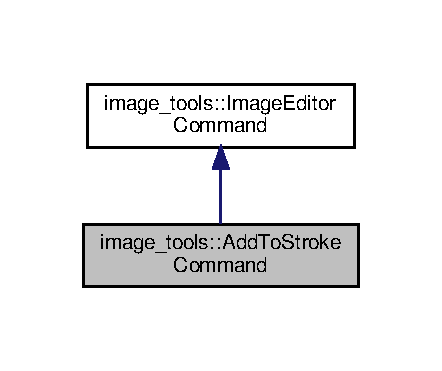
\includegraphics[width=212pt]{classimage__tools_1_1AddToStrokeCommand__inherit__graph}
\end{center}
\end{figure}


Collaboration diagram for image\+\_\+tools\+:\+:Add\+To\+Stroke\+Command\+:
\nopagebreak
\begin{figure}[H]
\begin{center}
\leavevmode
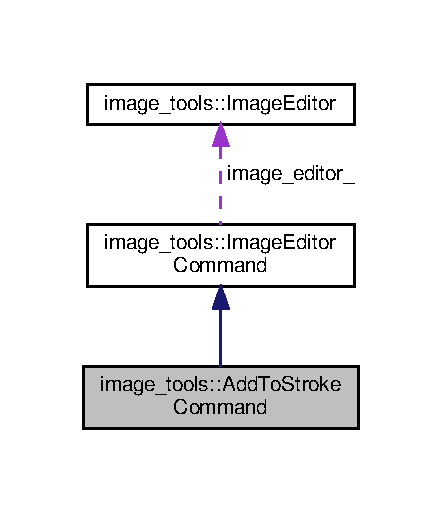
\includegraphics[width=212pt]{classimage__tools_1_1AddToStrokeCommand__coll__graph}
\end{center}
\end{figure}
\subsection*{Public Member Functions}
\begin{DoxyCompactItemize}
\item 
\mbox{\Hypertarget{classimage__tools_1_1AddToStrokeCommand_a8e68a32c1e8812aa540719c2e21f8242}\label{classimage__tools_1_1AddToStrokeCommand_a8e68a32c1e8812aa540719c2e21f8242}} 
{\bfseries Add\+To\+Stroke\+Command} (\hyperlink{classimage__tools_1_1ImageEditor}{Image\+Editor} $\ast$image\+\_\+editor, int x, int y)
\item 
\mbox{\Hypertarget{classimage__tools_1_1AddToStrokeCommand_ad02db74e4d5d87b6dc5cad5cfc9dc9ec}\label{classimage__tools_1_1AddToStrokeCommand_ad02db74e4d5d87b6dc5cad5cfc9dc9ec}} 
void {\bfseries Execute} () override
\end{DoxyCompactItemize}
\subsection*{Additional Inherited Members}


\subsection{Detailed Description}
Specific command for adding to the most recently started stroke. 

The documentation for this class was generated from the following files\+:\begin{DoxyCompactItemize}
\item 
src/mia/image\+\_\+editor\+\_\+commands.\+h\item 
src/mia/image\+\_\+editor\+\_\+commands.\+cc\end{DoxyCompactItemize}

\hypertarget{classimage__tools_1_1BlurFilterCommand}{}\section{image\+\_\+tools\+:\+:Blur\+Filter\+Command Class Reference}
\label{classimage__tools_1_1BlurFilterCommand}\index{image\+\_\+tools\+::\+Blur\+Filter\+Command@{image\+\_\+tools\+::\+Blur\+Filter\+Command}}


{\ttfamily \#include $<$image\+\_\+editor\+\_\+commands.\+h$>$}



Inheritance diagram for image\+\_\+tools\+:\+:Blur\+Filter\+Command\+:
\nopagebreak
\begin{figure}[H]
\begin{center}
\leavevmode
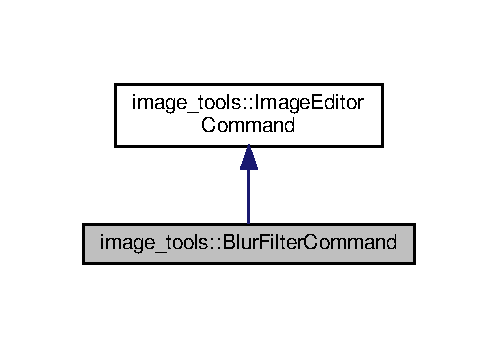
\includegraphics[width=239pt]{classimage__tools_1_1BlurFilterCommand__inherit__graph}
\end{center}
\end{figure}


Collaboration diagram for image\+\_\+tools\+:\+:Blur\+Filter\+Command\+:
\nopagebreak
\begin{figure}[H]
\begin{center}
\leavevmode
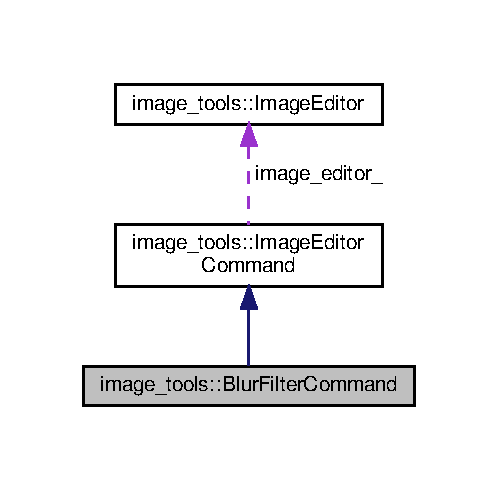
\includegraphics[width=239pt]{classimage__tools_1_1BlurFilterCommand__coll__graph}
\end{center}
\end{figure}
\subsection*{Public Member Functions}
\begin{DoxyCompactItemize}
\item 
\mbox{\Hypertarget{classimage__tools_1_1BlurFilterCommand_a20f12622e336a6ede53a169fb62882c6}\label{classimage__tools_1_1BlurFilterCommand_a20f12622e336a6ede53a169fb62882c6}} 
{\bfseries Blur\+Filter\+Command} (\hyperlink{classimage__tools_1_1ImageEditor}{Image\+Editor} $\ast$image\+\_\+editor, float radius)
\item 
\mbox{\Hypertarget{classimage__tools_1_1BlurFilterCommand_a14974e1b3c6eb5a810d0fe872a4f4a20}\label{classimage__tools_1_1BlurFilterCommand_a14974e1b3c6eb5a810d0fe872a4f4a20}} 
void {\bfseries Execute} () override
\end{DoxyCompactItemize}
\subsection*{Additional Inherited Members}


\subsection{Detailed Description}
Specific command for executing a blur filter. 

The documentation for this class was generated from the following files\+:\begin{DoxyCompactItemize}
\item 
src/mia/image\+\_\+editor\+\_\+commands.\+h\item 
src/mia/image\+\_\+editor\+\_\+commands.\+cc\end{DoxyCompactItemize}

\hypertarget{classimage__tools_1_1ChannelsFilterCommand}{}\section{image\+\_\+tools\+:\+:Channels\+Filter\+Command Class Reference}
\label{classimage__tools_1_1ChannelsFilterCommand}\index{image\+\_\+tools\+::\+Channels\+Filter\+Command@{image\+\_\+tools\+::\+Channels\+Filter\+Command}}


{\ttfamily \#include $<$image\+\_\+editor\+\_\+commands.\+h$>$}



Inheritance diagram for image\+\_\+tools\+:\+:Channels\+Filter\+Command\+:
\nopagebreak
\begin{figure}[H]
\begin{center}
\leavevmode
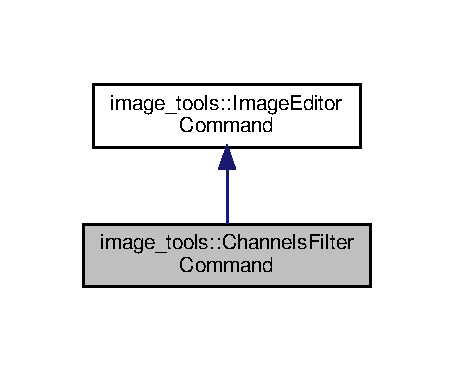
\includegraphics[width=218pt]{classimage__tools_1_1ChannelsFilterCommand__inherit__graph}
\end{center}
\end{figure}


Collaboration diagram for image\+\_\+tools\+:\+:Channels\+Filter\+Command\+:
\nopagebreak
\begin{figure}[H]
\begin{center}
\leavevmode
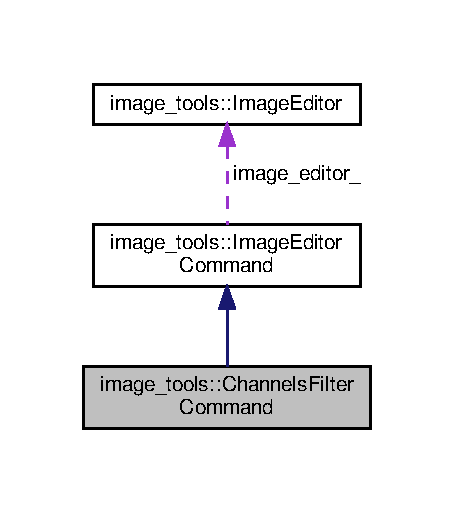
\includegraphics[width=218pt]{classimage__tools_1_1ChannelsFilterCommand__coll__graph}
\end{center}
\end{figure}
\subsection*{Public Member Functions}
\begin{DoxyCompactItemize}
\item 
\mbox{\Hypertarget{classimage__tools_1_1ChannelsFilterCommand_a7fd606c74e4855cc9a886524d89ff743}\label{classimage__tools_1_1ChannelsFilterCommand_a7fd606c74e4855cc9a886524d89ff743}} 
{\bfseries Channels\+Filter\+Command} (\hyperlink{classimage__tools_1_1ImageEditor}{Image\+Editor} $\ast$image\+\_\+editor, float red\+\_\+scale, float green\+\_\+scale, float blue\+\_\+scale)
\item 
\mbox{\Hypertarget{classimage__tools_1_1ChannelsFilterCommand_aeb73190ed2ee6b86dc641c1fe4e0c728}\label{classimage__tools_1_1ChannelsFilterCommand_aeb73190ed2ee6b86dc641c1fe4e0c728}} 
void {\bfseries Execute} () override
\end{DoxyCompactItemize}
\subsection*{Additional Inherited Members}


\subsection{Detailed Description}
Specific command for executing the channels filter. 

The documentation for this class was generated from the following files\+:\begin{DoxyCompactItemize}
\item 
src/mia/image\+\_\+editor\+\_\+commands.\+h\item 
src/mia/image\+\_\+editor\+\_\+commands.\+cc\end{DoxyCompactItemize}

\hypertarget{classimage__tools_1_1ColorData}{}\section{image\+\_\+tools\+:\+:Color\+Data Class Reference}
\label{classimage__tools_1_1ColorData}\index{image\+\_\+tools\+::\+Color\+Data@{image\+\_\+tools\+::\+Color\+Data}}


This color data class stores color in floating point format. The Red, Green, Blue, and Alpha channels range from 0.\+0 to 1.\+0.  




{\ttfamily \#include $<$color\+\_\+data.\+h$>$}

\subsection*{Public Member Functions}
\begin{DoxyCompactItemize}
\item 
\mbox{\Hypertarget{classimage__tools_1_1ColorData_ad64a66f681d0e502c2416e0bfcb86d14}\label{classimage__tools_1_1ColorData_ad64a66f681d0e502c2416e0bfcb86d14}} 
{\bfseries Color\+Data} (float r, float g, float b)
\item 
\mbox{\Hypertarget{classimage__tools_1_1ColorData_a20782ba5f82e73e731b87311da1bcd56}\label{classimage__tools_1_1ColorData_a20782ba5f82e73e731b87311da1bcd56}} 
{\bfseries Color\+Data} (float r, float g, float b, float a)
\item 
\mbox{\Hypertarget{classimage__tools_1_1ColorData_ad920899b7064bec8d8f252d8bf4d7cf9}\label{classimage__tools_1_1ColorData_ad920899b7064bec8d8f252d8bf4d7cf9}} 
float {\bfseries red} () const
\item 
\mbox{\Hypertarget{classimage__tools_1_1ColorData_a7848c06faf7797998cb83df818d6ab48}\label{classimage__tools_1_1ColorData_a7848c06faf7797998cb83df818d6ab48}} 
void {\bfseries set\+\_\+red} (float r)
\item 
\mbox{\Hypertarget{classimage__tools_1_1ColorData_aa26733d8617bc9033c0444db6b046fc3}\label{classimage__tools_1_1ColorData_aa26733d8617bc9033c0444db6b046fc3}} 
float {\bfseries green} () const
\item 
\mbox{\Hypertarget{classimage__tools_1_1ColorData_aae91ca399cd24ed86b15cf0d0b872786}\label{classimage__tools_1_1ColorData_aae91ca399cd24ed86b15cf0d0b872786}} 
void {\bfseries set\+\_\+green} (float g)
\item 
\mbox{\Hypertarget{classimage__tools_1_1ColorData_a9b1d04ed2d00ff017968bb43cf7b8075}\label{classimage__tools_1_1ColorData_a9b1d04ed2d00ff017968bb43cf7b8075}} 
float {\bfseries blue} () const
\item 
\mbox{\Hypertarget{classimage__tools_1_1ColorData_a97913efb23816200ba2de45f9123d962}\label{classimage__tools_1_1ColorData_a97913efb23816200ba2de45f9123d962}} 
void {\bfseries set\+\_\+blue} (float b)
\item 
\mbox{\Hypertarget{classimage__tools_1_1ColorData_a0f191463c70539bd414c38fc6e6db2b4}\label{classimage__tools_1_1ColorData_a0f191463c70539bd414c38fc6e6db2b4}} 
float {\bfseries alpha} () const
\item 
\mbox{\Hypertarget{classimage__tools_1_1ColorData_a4fe0c6683e81df186df950bf3a43d220}\label{classimage__tools_1_1ColorData_a4fe0c6683e81df186df950bf3a43d220}} 
void {\bfseries set\+\_\+alpha} (float a)
\item 
\mbox{\Hypertarget{classimage__tools_1_1ColorData_ac36f32461a63c77c0fdf99296e1d1faf}\label{classimage__tools_1_1ColorData_ac36f32461a63c77c0fdf99296e1d1faf}} 
float \hyperlink{classimage__tools_1_1ColorData_ac36f32461a63c77c0fdf99296e1d1faf}{Luminance} () const
\begin{DoxyCompactList}\small\item\em Calculates the \char`\"{}brightness\char`\"{} of the color according to a perceptual metric that weights the red, green, and blue components of the color non-\/uniformly to account for the non-\/uniformity of the human visual system. \end{DoxyCompactList}\item 
\mbox{\Hypertarget{classimage__tools_1_1ColorData_ae64129037eb8de589e8de9dbc45704a8}\label{classimage__tools_1_1ColorData_ae64129037eb8de589e8de9dbc45704a8}} 
void \hyperlink{classimage__tools_1_1ColorData_ae64129037eb8de589e8de9dbc45704a8}{Clamp} ()
\begin{DoxyCompactList}\small\item\em Clamps each channel of the color so that the data are within the range \mbox{[}0.\+0,1.\+0\mbox{]}. \end{DoxyCompactList}\end{DoxyCompactItemize}
\subsection*{Friends}
\begin{DoxyCompactItemize}
\item 
\mbox{\Hypertarget{classimage__tools_1_1ColorData_adf9a770243996e50282d248a4327f351}\label{classimage__tools_1_1ColorData_adf9a770243996e50282d248a4327f351}} 
\hyperlink{classimage__tools_1_1ColorData}{Color\+Data} {\bfseries operator$\ast$} (const \hyperlink{classimage__tools_1_1ColorData}{Color\+Data} \&a, float f)
\item 
\mbox{\Hypertarget{classimage__tools_1_1ColorData_afee00faf26189979b72f3854a17200ae}\label{classimage__tools_1_1ColorData_afee00faf26189979b72f3854a17200ae}} 
\hyperlink{classimage__tools_1_1ColorData}{Color\+Data} {\bfseries operator+} (const \hyperlink{classimage__tools_1_1ColorData}{Color\+Data} \&a, const \hyperlink{classimage__tools_1_1ColorData}{Color\+Data} \&b)
\item 
\mbox{\Hypertarget{classimage__tools_1_1ColorData_a799bd54f65a61569b5b968062ac0d37e}\label{classimage__tools_1_1ColorData_a799bd54f65a61569b5b968062ac0d37e}} 
\hyperlink{classimage__tools_1_1ColorData}{Color\+Data} {\bfseries operator-\/} (const \hyperlink{classimage__tools_1_1ColorData}{Color\+Data} \&a, const \hyperlink{classimage__tools_1_1ColorData}{Color\+Data} \&b)
\item 
bool \hyperlink{classimage__tools_1_1ColorData_a9dae9e77610393d100312c9d248f09cc}{operator==} (const \hyperlink{classimage__tools_1_1ColorData}{Color\+Data} \&a, const \hyperlink{classimage__tools_1_1ColorData}{Color\+Data} \&b)
\item 
bool \hyperlink{classimage__tools_1_1ColorData_a698ac263a286afe37e3b9ed0c5882c8c}{operator!=} (const \hyperlink{classimage__tools_1_1ColorData}{Color\+Data} \&a, const \hyperlink{classimage__tools_1_1ColorData}{Color\+Data} \&b)
\end{DoxyCompactItemize}


\subsection{Detailed Description}
This color data class stores color in floating point format. The Red, Green, Blue, and Alpha channels range from 0.\+0 to 1.\+0. 

\subsection{Friends And Related Function Documentation}
\mbox{\Hypertarget{classimage__tools_1_1ColorData_a698ac263a286afe37e3b9ed0c5882c8c}\label{classimage__tools_1_1ColorData_a698ac263a286afe37e3b9ed0c5882c8c}} 
\index{image\+\_\+tools\+::\+Color\+Data@{image\+\_\+tools\+::\+Color\+Data}!operator"!=@{operator"!=}}
\index{operator"!=@{operator"!=}!image\+\_\+tools\+::\+Color\+Data@{image\+\_\+tools\+::\+Color\+Data}}
\subsubsection{\texorpdfstring{operator"!=}{operator!=}}
{\footnotesize\ttfamily bool operator!= (\begin{DoxyParamCaption}\item[{const \hyperlink{classimage__tools_1_1ColorData}{Color\+Data} \&}]{a,  }\item[{const \hyperlink{classimage__tools_1_1ColorData}{Color\+Data} \&}]{b }\end{DoxyParamCaption})\hspace{0.3cm}{\ttfamily [friend]}}

Check for \char`\"{}inequality\char`\"{}, taking floating point imprecision into account \mbox{\Hypertarget{classimage__tools_1_1ColorData_a9dae9e77610393d100312c9d248f09cc}\label{classimage__tools_1_1ColorData_a9dae9e77610393d100312c9d248f09cc}} 
\index{image\+\_\+tools\+::\+Color\+Data@{image\+\_\+tools\+::\+Color\+Data}!operator==@{operator==}}
\index{operator==@{operator==}!image\+\_\+tools\+::\+Color\+Data@{image\+\_\+tools\+::\+Color\+Data}}
\subsubsection{\texorpdfstring{operator==}{operator==}}
{\footnotesize\ttfamily bool operator== (\begin{DoxyParamCaption}\item[{const \hyperlink{classimage__tools_1_1ColorData}{Color\+Data} \&}]{a,  }\item[{const \hyperlink{classimage__tools_1_1ColorData}{Color\+Data} \&}]{b }\end{DoxyParamCaption})\hspace{0.3cm}{\ttfamily [friend]}}

Check for \char`\"{}equality\char`\"{}, taking floating point imprecision into account 

The documentation for this class was generated from the following files\+:\begin{DoxyCompactItemize}
\item 
src/imagetools/color\+\_\+data.\+h\item 
src/imagetools/color\+\_\+data.\+cc\end{DoxyCompactItemize}

\hypertarget{classimage__tools_1_1CommandLineProcessor}{}\section{image\+\_\+tools\+:\+:Command\+Line\+Processor Class Reference}
\label{classimage__tools_1_1CommandLineProcessor}\index{image\+\_\+tools\+::\+Command\+Line\+Processor@{image\+\_\+tools\+::\+Command\+Line\+Processor}}


Processes a series of input(s) from the user and applies the change(s) to an image without a G\+UI.  




{\ttfamily \#include $<$command\+\_\+line\+\_\+processor.\+h$>$}

\subsection*{Public Member Functions}
\begin{DoxyCompactItemize}
\item 
\mbox{\Hypertarget{classimage__tools_1_1CommandLineProcessor_aaa6f203a5fdc9687bc4c7e834e113625}\label{classimage__tools_1_1CommandLineProcessor_aaa6f203a5fdc9687bc4c7e834e113625}} 
void \hyperlink{classimage__tools_1_1CommandLineProcessor_aaa6f203a5fdc9687bc4c7e834e113625}{Process\+Command\+Line} (int argc, char $\ast$argv\mbox{[}$\,$\mbox{]})
\begin{DoxyCompactList}\small\item\em Checks to see if the input(s) are valid. \end{DoxyCompactList}\item 
\mbox{\Hypertarget{classimage__tools_1_1CommandLineProcessor_a2297f0a67e3958ec5e2260f33cf42daf}\label{classimage__tools_1_1CommandLineProcessor_a2297f0a67e3958ec5e2260f33cf42daf}} 
void \hyperlink{classimage__tools_1_1CommandLineProcessor_a2297f0a67e3958ec5e2260f33cf42daf}{Print\+Error\+Message} ()
\begin{DoxyCompactList}\small\item\em Prints out a help message to the terminal if a user inputs an invalid command or if the user inputs \char`\"{}-\/h\char`\"{}. \end{DoxyCompactList}\end{DoxyCompactItemize}


\subsection{Detailed Description}
Processes a series of input(s) from the user and applies the change(s) to an image without a G\+UI. 

The documentation for this class was generated from the following files\+:\begin{DoxyCompactItemize}
\item 
src/mia/command\+\_\+line\+\_\+processor.\+h\item 
src/mia/command\+\_\+line\+\_\+processor.\+cc\end{DoxyCompactItemize}

\hypertarget{classimage__tools_1_1ConvolutionFilter}{}\section{image\+\_\+tools\+:\+:Convolution\+Filter Class Reference}
\label{classimage__tools_1_1ConvolutionFilter}\index{image\+\_\+tools\+::\+Convolution\+Filter@{image\+\_\+tools\+::\+Convolution\+Filter}}


Inherits from the \hyperlink{classimage__tools_1_1Filter}{Filter} class to implement the following convolution filters\+: Blur, Edge Detect, Motion Blur, and Sharpen.  




{\ttfamily \#include $<$convolution\+\_\+filter.\+h$>$}



Inheritance diagram for image\+\_\+tools\+:\+:Convolution\+Filter\+:
\nopagebreak
\begin{figure}[H]
\begin{center}
\leavevmode
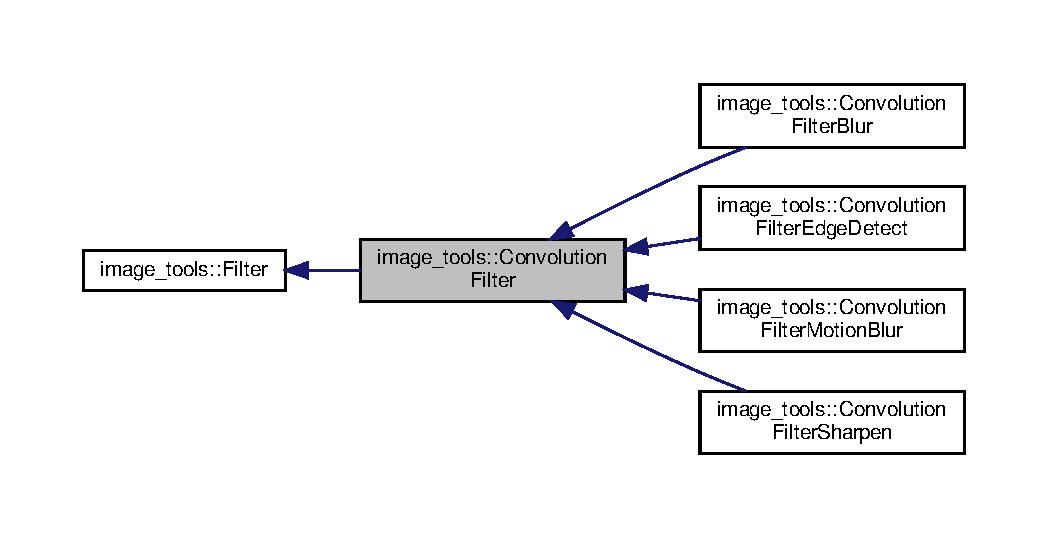
\includegraphics[width=350pt]{classimage__tools_1_1ConvolutionFilter__inherit__graph}
\end{center}
\end{figure}


Collaboration diagram for image\+\_\+tools\+:\+:Convolution\+Filter\+:
\nopagebreak
\begin{figure}[H]
\begin{center}
\leavevmode
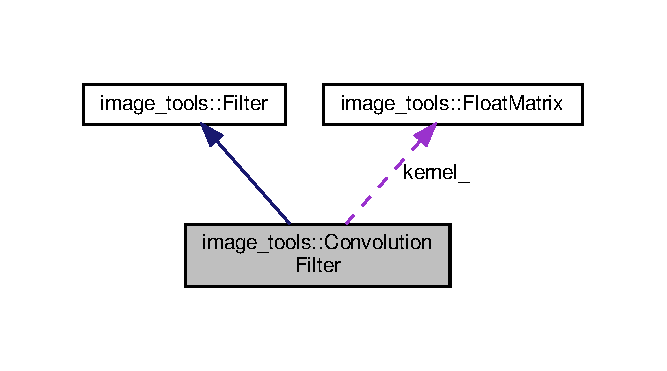
\includegraphics[width=320pt]{classimage__tools_1_1ConvolutionFilter__coll__graph}
\end{center}
\end{figure}
\subsection*{Public Member Functions}
\begin{DoxyCompactItemize}
\item 
\mbox{\Hypertarget{classimage__tools_1_1ConvolutionFilter_aac988aaa5e27213ea874d9bd3eb1dbdb}\label{classimage__tools_1_1ConvolutionFilter_aac988aaa5e27213ea874d9bd3eb1dbdb}} 
virtual \hyperlink{classimage__tools_1_1FloatMatrix}{Float\+Matrix} $\ast$ \hyperlink{classimage__tools_1_1ConvolutionFilter_aac988aaa5e27213ea874d9bd3eb1dbdb}{Create\+Kernel} ()
\begin{DoxyCompactList}\small\item\em Will be overriden by the convolution filters. \end{DoxyCompactList}\item 
\mbox{\Hypertarget{classimage__tools_1_1ConvolutionFilter_a49be1e3b2affd935378eb12d4f240048}\label{classimage__tools_1_1ConvolutionFilter_a49be1e3b2affd935378eb12d4f240048}} 
void \hyperlink{classimage__tools_1_1ConvolutionFilter_a49be1e3b2affd935378eb12d4f240048}{Setup\+Filter} () override
\begin{DoxyCompactList}\small\item\em Creates a default kernel. \end{DoxyCompactList}\item 
\hyperlink{classimage__tools_1_1ColorData}{Color\+Data} \hyperlink{classimage__tools_1_1ConvolutionFilter_a2d35a2e2a2d1303d0a6824b16406d97b}{Calculate\+Filtered\+Pixel} (\hyperlink{classimage__tools_1_1PixelBuffer}{Pixel\+Buffer} $\ast$buffer, int x, int y) override
\item 
\mbox{\Hypertarget{classimage__tools_1_1ConvolutionFilter_a67668b9a965491b1184ce645ac3250ed}\label{classimage__tools_1_1ConvolutionFilter_a67668b9a965491b1184ce645ac3250ed}} 
void \hyperlink{classimage__tools_1_1ConvolutionFilter_a67668b9a965491b1184ce645ac3250ed}{Cleanup\+Filter} () override
\begin{DoxyCompactList}\small\item\em Deletes pointer value. \end{DoxyCompactList}\item 
bool \hyperlink{classimage__tools_1_1ConvolutionFilter_aef03779d74d96173880d93d06c7bd6b6}{can\+\_\+copy\+\_\+in\+\_\+place} () override
\end{DoxyCompactItemize}
\subsection*{Protected Attributes}
\begin{DoxyCompactItemize}
\item 
\mbox{\Hypertarget{classimage__tools_1_1ConvolutionFilter_a4ef900e0e03585707fce8b71afd40c5d}\label{classimage__tools_1_1ConvolutionFilter_a4ef900e0e03585707fce8b71afd40c5d}} 
\hyperlink{classimage__tools_1_1FloatMatrix}{Float\+Matrix} $\ast$ {\bfseries kernel\+\_\+}
\end{DoxyCompactItemize}


\subsection{Detailed Description}
Inherits from the \hyperlink{classimage__tools_1_1Filter}{Filter} class to implement the following convolution filters\+: Blur, Edge Detect, Motion Blur, and Sharpen. 

\subsection{Member Function Documentation}
\mbox{\Hypertarget{classimage__tools_1_1ConvolutionFilter_a2d35a2e2a2d1303d0a6824b16406d97b}\label{classimage__tools_1_1ConvolutionFilter_a2d35a2e2a2d1303d0a6824b16406d97b}} 
\index{image\+\_\+tools\+::\+Convolution\+Filter@{image\+\_\+tools\+::\+Convolution\+Filter}!Calculate\+Filtered\+Pixel@{Calculate\+Filtered\+Pixel}}
\index{Calculate\+Filtered\+Pixel@{Calculate\+Filtered\+Pixel}!image\+\_\+tools\+::\+Convolution\+Filter@{image\+\_\+tools\+::\+Convolution\+Filter}}
\subsubsection{\texorpdfstring{Calculate\+Filtered\+Pixel()}{CalculateFilteredPixel()}}
{\footnotesize\ttfamily \hyperlink{classimage__tools_1_1ColorData}{Color\+Data} image\+\_\+tools\+::\+Convolution\+Filter\+::\+Calculate\+Filtered\+Pixel (\begin{DoxyParamCaption}\item[{\hyperlink{classimage__tools_1_1PixelBuffer}{Pixel\+Buffer} $\ast$}]{buffer,  }\item[{int}]{x,  }\item[{int}]{y }\end{DoxyParamCaption})\hspace{0.3cm}{\ttfamily [override]}, {\ttfamily [virtual]}}

Repurposed code to calculate each filtered pixel. Source\+: \href{https://lodev.org/cgtutor/filtering.html}{\tt https\+://lodev.\+org/cgtutor/filtering.\+html}. 

Reimplemented from \hyperlink{classimage__tools_1_1Filter_a68d38fa12b87e20b81090cb380c0a307}{image\+\_\+tools\+::\+Filter}.

\mbox{\Hypertarget{classimage__tools_1_1ConvolutionFilter_aef03779d74d96173880d93d06c7bd6b6}\label{classimage__tools_1_1ConvolutionFilter_aef03779d74d96173880d93d06c7bd6b6}} 
\index{image\+\_\+tools\+::\+Convolution\+Filter@{image\+\_\+tools\+::\+Convolution\+Filter}!can\+\_\+copy\+\_\+in\+\_\+place@{can\+\_\+copy\+\_\+in\+\_\+place}}
\index{can\+\_\+copy\+\_\+in\+\_\+place@{can\+\_\+copy\+\_\+in\+\_\+place}!image\+\_\+tools\+::\+Convolution\+Filter@{image\+\_\+tools\+::\+Convolution\+Filter}}
\subsubsection{\texorpdfstring{can\+\_\+copy\+\_\+in\+\_\+place()}{can\_copy\_in\_place()}}
{\footnotesize\ttfamily bool image\+\_\+tools\+::\+Convolution\+Filter\+::can\+\_\+copy\+\_\+in\+\_\+place (\begin{DoxyParamCaption}{ }\end{DoxyParamCaption})\hspace{0.3cm}{\ttfamily [override]}, {\ttfamily [virtual]}}

Convolution Filters require a copy buffer since they cannot be copied in place. 

Reimplemented from \hyperlink{classimage__tools_1_1Filter_abb21c6ce1f09a4ce4fbd38255c44d281}{image\+\_\+tools\+::\+Filter}.



The documentation for this class was generated from the following files\+:\begin{DoxyCompactItemize}
\item 
src/imagetools/convolution\+\_\+filter.\+h\item 
src/imagetools/convolution\+\_\+filter.\+cc\end{DoxyCompactItemize}

\hypertarget{classimage__tools_1_1ConvolutionFilterBlur}{}\section{image\+\_\+tools\+:\+:Convolution\+Filter\+Blur Class Reference}
\label{classimage__tools_1_1ConvolutionFilterBlur}\index{image\+\_\+tools\+::\+Convolution\+Filter\+Blur@{image\+\_\+tools\+::\+Convolution\+Filter\+Blur}}


Implements a blur filter using a corresponding blur kernel.  




{\ttfamily \#include $<$convolution\+\_\+filter\+\_\+blur.\+h$>$}



Inheritance diagram for image\+\_\+tools\+:\+:Convolution\+Filter\+Blur\+:
\nopagebreak
\begin{figure}[H]
\begin{center}
\leavevmode
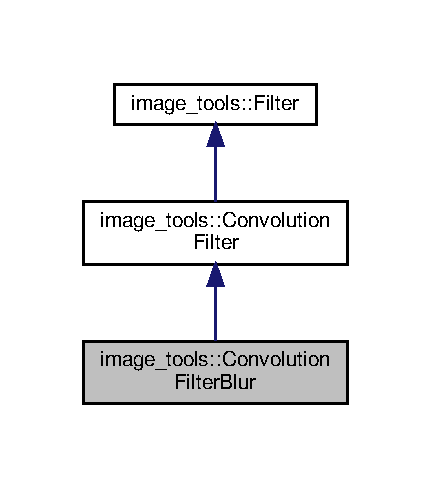
\includegraphics[width=207pt]{classimage__tools_1_1ConvolutionFilterBlur__inherit__graph}
\end{center}
\end{figure}


Collaboration diagram for image\+\_\+tools\+:\+:Convolution\+Filter\+Blur\+:
\nopagebreak
\begin{figure}[H]
\begin{center}
\leavevmode
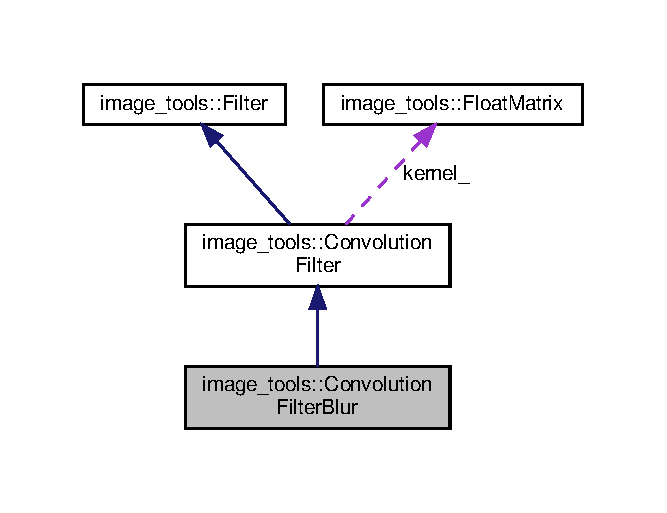
\includegraphics[width=320pt]{classimage__tools_1_1ConvolutionFilterBlur__coll__graph}
\end{center}
\end{figure}
\subsection*{Public Member Functions}
\begin{DoxyCompactItemize}
\item 
\mbox{\Hypertarget{classimage__tools_1_1ConvolutionFilterBlur_a8b00c3c274763a4f9cd67a0a18d544e8}\label{classimage__tools_1_1ConvolutionFilterBlur_a8b00c3c274763a4f9cd67a0a18d544e8}} 
\hyperlink{classimage__tools_1_1ConvolutionFilterBlur_a8b00c3c274763a4f9cd67a0a18d544e8}{Convolution\+Filter\+Blur} ()
\begin{DoxyCompactList}\small\item\em Defaults to radius=5.\+0. \end{DoxyCompactList}\item 
\mbox{\Hypertarget{classimage__tools_1_1ConvolutionFilterBlur_a2f809172d1b0ea253ac9259db4d7acba}\label{classimage__tools_1_1ConvolutionFilterBlur_a2f809172d1b0ea253ac9259db4d7acba}} 
void {\bfseries Set\+Rad} (float radius)
\item 
\mbox{\Hypertarget{classimage__tools_1_1ConvolutionFilterBlur_a310546bd12dcc8894f0af414677b2b07}\label{classimage__tools_1_1ConvolutionFilterBlur_a310546bd12dcc8894f0af414677b2b07}} 
\hyperlink{classimage__tools_1_1FloatMatrix}{Float\+Matrix} $\ast$ \hyperlink{classimage__tools_1_1ConvolutionFilterBlur_a310546bd12dcc8894f0af414677b2b07}{Create\+Kernel} () override
\begin{DoxyCompactList}\small\item\em Will be overriden by the convolution filters. \end{DoxyCompactList}\end{DoxyCompactItemize}
\subsection*{Additional Inherited Members}


\subsection{Detailed Description}
Implements a blur filter using a corresponding blur kernel. 

The documentation for this class was generated from the following files\+:\begin{DoxyCompactItemize}
\item 
src/imagetools/convolution\+\_\+filter\+\_\+blur.\+h\item 
src/imagetools/convolution\+\_\+filter\+\_\+blur.\+cc\end{DoxyCompactItemize}

\hypertarget{classimage__tools_1_1ConvolutionFilterEdgeDetect}{}\section{image\+\_\+tools\+:\+:Convolution\+Filter\+Edge\+Detect Class Reference}
\label{classimage__tools_1_1ConvolutionFilterEdgeDetect}\index{image\+\_\+tools\+::\+Convolution\+Filter\+Edge\+Detect@{image\+\_\+tools\+::\+Convolution\+Filter\+Edge\+Detect}}


Implements a edge detecting filter using a corresponding edge detecting kernel.  




{\ttfamily \#include $<$convolution\+\_\+filter\+\_\+edge\+\_\+detect.\+h$>$}



Inheritance diagram for image\+\_\+tools\+:\+:Convolution\+Filter\+Edge\+Detect\+:
\nopagebreak
\begin{figure}[H]
\begin{center}
\leavevmode
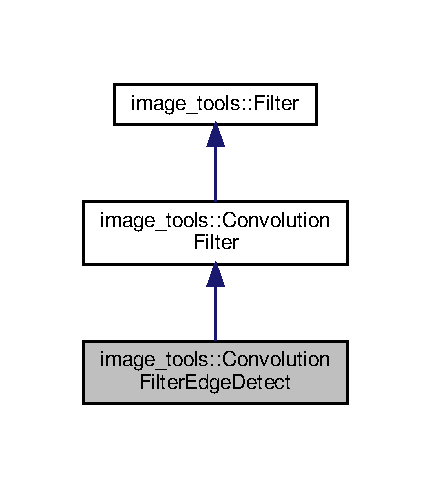
\includegraphics[width=207pt]{classimage__tools_1_1ConvolutionFilterEdgeDetect__inherit__graph}
\end{center}
\end{figure}


Collaboration diagram for image\+\_\+tools\+:\+:Convolution\+Filter\+Edge\+Detect\+:
\nopagebreak
\begin{figure}[H]
\begin{center}
\leavevmode
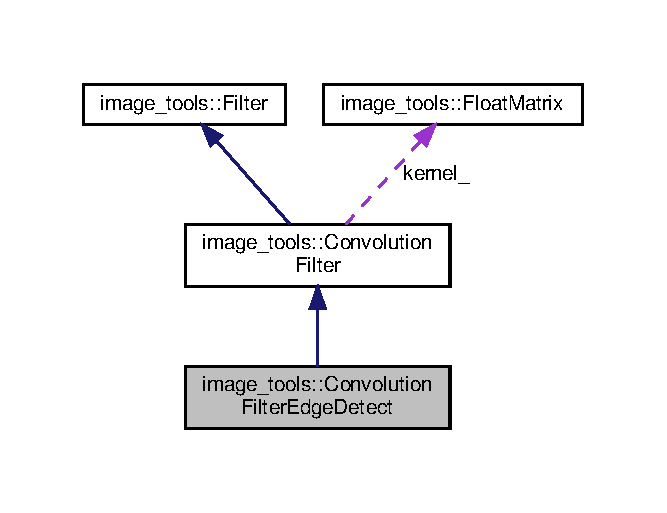
\includegraphics[width=320pt]{classimage__tools_1_1ConvolutionFilterEdgeDetect__coll__graph}
\end{center}
\end{figure}
\subsection*{Public Member Functions}
\begin{DoxyCompactItemize}
\item 
\mbox{\Hypertarget{classimage__tools_1_1ConvolutionFilterEdgeDetect_ae2ec1313b3a53c6542ce369321ebab21}\label{classimage__tools_1_1ConvolutionFilterEdgeDetect_ae2ec1313b3a53c6542ce369321ebab21}} 
\hyperlink{classimage__tools_1_1FloatMatrix}{Float\+Matrix} $\ast$ \hyperlink{classimage__tools_1_1ConvolutionFilterEdgeDetect_ae2ec1313b3a53c6542ce369321ebab21}{Create\+Kernel} () override
\begin{DoxyCompactList}\small\item\em Will be overriden by the convolution filters. \end{DoxyCompactList}\end{DoxyCompactItemize}
\subsection*{Additional Inherited Members}


\subsection{Detailed Description}
Implements a edge detecting filter using a corresponding edge detecting kernel. 

The documentation for this class was generated from the following files\+:\begin{DoxyCompactItemize}
\item 
src/imagetools/convolution\+\_\+filter\+\_\+edge\+\_\+detect.\+h\item 
src/imagetools/convolution\+\_\+filter\+\_\+edge\+\_\+detect.\+cc\end{DoxyCompactItemize}

\hypertarget{classimage__tools_1_1ConvolutionFilterMotionBlur}{}\section{image\+\_\+tools\+:\+:Convolution\+Filter\+Motion\+Blur Class Reference}
\label{classimage__tools_1_1ConvolutionFilterMotionBlur}\index{image\+\_\+tools\+::\+Convolution\+Filter\+Motion\+Blur@{image\+\_\+tools\+::\+Convolution\+Filter\+Motion\+Blur}}


Implements a motion blur filter using a corresponding motion blur kernel.  




{\ttfamily \#include $<$convolution\+\_\+filter\+\_\+motion\+\_\+blur.\+h$>$}



Inheritance diagram for image\+\_\+tools\+:\+:Convolution\+Filter\+Motion\+Blur\+:
\nopagebreak
\begin{figure}[H]
\begin{center}
\leavevmode
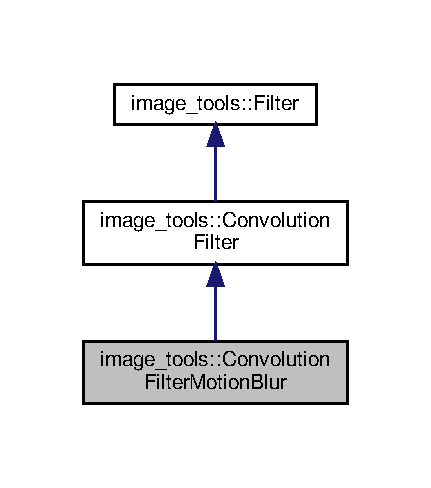
\includegraphics[width=207pt]{classimage__tools_1_1ConvolutionFilterMotionBlur__inherit__graph}
\end{center}
\end{figure}


Collaboration diagram for image\+\_\+tools\+:\+:Convolution\+Filter\+Motion\+Blur\+:
\nopagebreak
\begin{figure}[H]
\begin{center}
\leavevmode
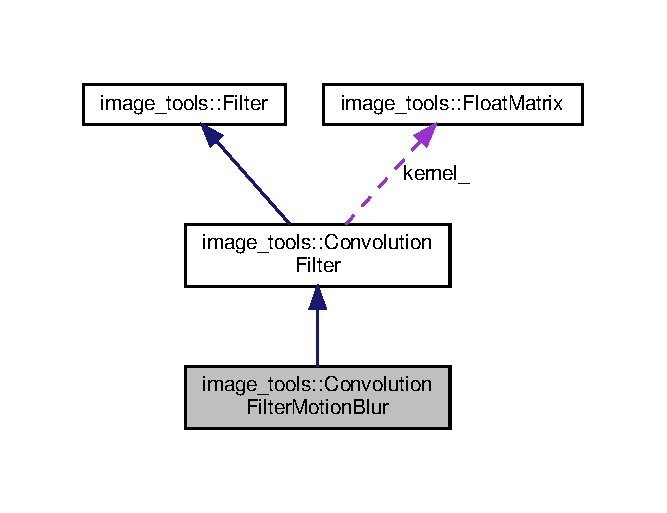
\includegraphics[width=320pt]{classimage__tools_1_1ConvolutionFilterMotionBlur__coll__graph}
\end{center}
\end{figure}
\subsection*{Public Member Functions}
\begin{DoxyCompactItemize}
\item 
\mbox{\Hypertarget{classimage__tools_1_1ConvolutionFilterMotionBlur_aca448e3ff4e2518444cab5a4e897a94d}\label{classimage__tools_1_1ConvolutionFilterMotionBlur_aca448e3ff4e2518444cab5a4e897a94d}} 
\hyperlink{classimage__tools_1_1ConvolutionFilterMotionBlur_aca448e3ff4e2518444cab5a4e897a94d}{Convolution\+Filter\+Motion\+Blur} ()
\begin{DoxyCompactList}\small\item\em Defaults to radius=5.\+0 and dir=\char`\"{}\+North/\+South\char`\"{}. \end{DoxyCompactList}\item 
void \hyperlink{classimage__tools_1_1ConvolutionFilterMotionBlur_afceed9724dbe3579f3affe5c2eff8b0d}{Set\+Values} (float radius, std\+::string dir)
\item 
\mbox{\Hypertarget{classimage__tools_1_1ConvolutionFilterMotionBlur_a745b24f809059b933c1c01322fa01217}\label{classimage__tools_1_1ConvolutionFilterMotionBlur_a745b24f809059b933c1c01322fa01217}} 
\hyperlink{classimage__tools_1_1FloatMatrix}{Float\+Matrix} $\ast$ \hyperlink{classimage__tools_1_1ConvolutionFilterMotionBlur_a745b24f809059b933c1c01322fa01217}{Create\+Kernel} () override
\begin{DoxyCompactList}\small\item\em Will be overriden by the convolution filters. \end{DoxyCompactList}\end{DoxyCompactItemize}
\subsection*{Additional Inherited Members}


\subsection{Detailed Description}
Implements a motion blur filter using a corresponding motion blur kernel. 

\subsection{Member Function Documentation}
\mbox{\Hypertarget{classimage__tools_1_1ConvolutionFilterMotionBlur_afceed9724dbe3579f3affe5c2eff8b0d}\label{classimage__tools_1_1ConvolutionFilterMotionBlur_afceed9724dbe3579f3affe5c2eff8b0d}} 
\index{image\+\_\+tools\+::\+Convolution\+Filter\+Motion\+Blur@{image\+\_\+tools\+::\+Convolution\+Filter\+Motion\+Blur}!Set\+Values@{Set\+Values}}
\index{Set\+Values@{Set\+Values}!image\+\_\+tools\+::\+Convolution\+Filter\+Motion\+Blur@{image\+\_\+tools\+::\+Convolution\+Filter\+Motion\+Blur}}
\subsubsection{\texorpdfstring{Set\+Values()}{SetValues()}}
{\footnotesize\ttfamily void image\+\_\+tools\+::\+Convolution\+Filter\+Motion\+Blur\+::\+Set\+Values (\begin{DoxyParamCaption}\item[{float}]{radius,  }\item[{std\+::string}]{dir }\end{DoxyParamCaption})}

The direction of the blur is determined by the string passed to this method. There are four possible blur directions\+: \char`\"{}\+North/\+South\char`\"{}, \char`\"{}\+East/\+West\char`\"{}, \char`\"{}\+Northeast/\+Southwest\char`\"{} and \char`\"{}\+Northwest/\+Southeast\char`\"{}. 

The documentation for this class was generated from the following files\+:\begin{DoxyCompactItemize}
\item 
src/imagetools/convolution\+\_\+filter\+\_\+motion\+\_\+blur.\+h\item 
src/imagetools/convolution\+\_\+filter\+\_\+motion\+\_\+blur.\+cc\end{DoxyCompactItemize}

\hypertarget{classimage__tools_1_1ConvolutionFilterSharpen}{}\section{image\+\_\+tools\+:\+:Convolution\+Filter\+Sharpen Class Reference}
\label{classimage__tools_1_1ConvolutionFilterSharpen}\index{image\+\_\+tools\+::\+Convolution\+Filter\+Sharpen@{image\+\_\+tools\+::\+Convolution\+Filter\+Sharpen}}


Implements a sharpening filter using a corresponding sharpening kernel.  




{\ttfamily \#include $<$convolution\+\_\+filter\+\_\+sharpen.\+h$>$}



Inheritance diagram for image\+\_\+tools\+:\+:Convolution\+Filter\+Sharpen\+:
\nopagebreak
\begin{figure}[H]
\begin{center}
\leavevmode
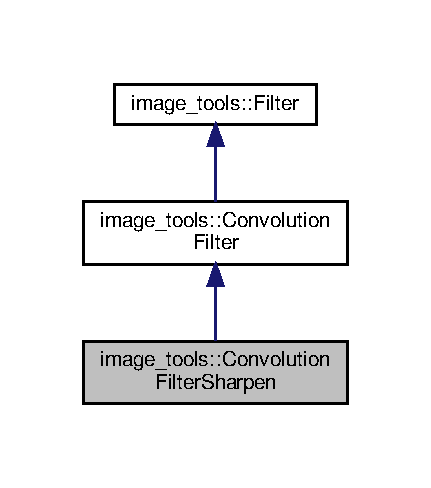
\includegraphics[width=207pt]{classimage__tools_1_1ConvolutionFilterSharpen__inherit__graph}
\end{center}
\end{figure}


Collaboration diagram for image\+\_\+tools\+:\+:Convolution\+Filter\+Sharpen\+:
\nopagebreak
\begin{figure}[H]
\begin{center}
\leavevmode
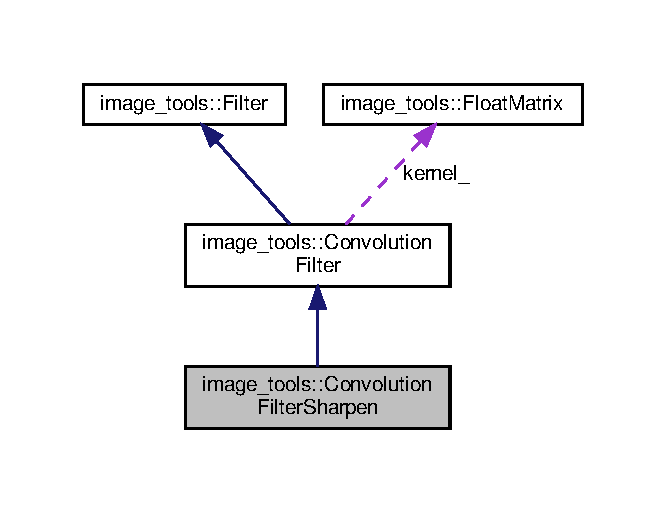
\includegraphics[width=320pt]{classimage__tools_1_1ConvolutionFilterSharpen__coll__graph}
\end{center}
\end{figure}
\subsection*{Public Member Functions}
\begin{DoxyCompactItemize}
\item 
\mbox{\Hypertarget{classimage__tools_1_1ConvolutionFilterSharpen_a4c8d5b2af0abf9b6582a05ad85f797fb}\label{classimage__tools_1_1ConvolutionFilterSharpen_a4c8d5b2af0abf9b6582a05ad85f797fb}} 
{\bfseries Convolution\+Filter\+Sharpen} (float radius)
\item 
\mbox{\Hypertarget{classimage__tools_1_1ConvolutionFilterSharpen_a38b78bc76570019a9f01618b37f68436}\label{classimage__tools_1_1ConvolutionFilterSharpen_a38b78bc76570019a9f01618b37f68436}} 
\hyperlink{classimage__tools_1_1ConvolutionFilterSharpen_a38b78bc76570019a9f01618b37f68436}{Convolution\+Filter\+Sharpen} ()
\begin{DoxyCompactList}\small\item\em Defaults to radius=5.\+0. \end{DoxyCompactList}\item 
\mbox{\Hypertarget{classimage__tools_1_1ConvolutionFilterSharpen_a39a6a428afbbdf6d9cf9f1971a2c468d}\label{classimage__tools_1_1ConvolutionFilterSharpen_a39a6a428afbbdf6d9cf9f1971a2c468d}} 
\hyperlink{classimage__tools_1_1FloatMatrix}{Float\+Matrix} $\ast$ \hyperlink{classimage__tools_1_1ConvolutionFilterSharpen_a39a6a428afbbdf6d9cf9f1971a2c468d}{Create\+Kernel} () override
\begin{DoxyCompactList}\small\item\em Will be overriden by the convolution filters. \end{DoxyCompactList}\item 
\mbox{\Hypertarget{classimage__tools_1_1ConvolutionFilterSharpen_afe4917632a0d56d0585cdcc953fd2791}\label{classimage__tools_1_1ConvolutionFilterSharpen_afe4917632a0d56d0585cdcc953fd2791}} 
bool {\bfseries convolve\+\_\+alpha} () const
\item 
\mbox{\Hypertarget{classimage__tools_1_1ConvolutionFilterSharpen_a1ea157e1dec999dc31ba1a0ac1479830}\label{classimage__tools_1_1ConvolutionFilterSharpen_a1ea157e1dec999dc31ba1a0ac1479830}} 
float {\bfseries radius} ()
\item 
\mbox{\Hypertarget{classimage__tools_1_1ConvolutionFilterSharpen_a8f4fb8f5f622e7bd91f8fa9208f11d16}\label{classimage__tools_1_1ConvolutionFilterSharpen_a8f4fb8f5f622e7bd91f8fa9208f11d16}} 
void {\bfseries set\+\_\+radius} (float r)
\end{DoxyCompactItemize}
\subsection*{Additional Inherited Members}


\subsection{Detailed Description}
Implements a sharpening filter using a corresponding sharpening kernel. 

The documentation for this class was generated from the following files\+:\begin{DoxyCompactItemize}
\item 
src/imagetools/convolution\+\_\+filter\+\_\+sharpen.\+h\item 
src/imagetools/convolution\+\_\+filter\+\_\+sharpen.\+cc\end{DoxyCompactItemize}

\hypertarget{classimage__tools_1_1EdgeFilterCommand}{}\section{image\+\_\+tools\+:\+:Edge\+Filter\+Command Class Reference}
\label{classimage__tools_1_1EdgeFilterCommand}\index{image\+\_\+tools\+::\+Edge\+Filter\+Command@{image\+\_\+tools\+::\+Edge\+Filter\+Command}}


{\ttfamily \#include $<$image\+\_\+editor\+\_\+commands.\+h$>$}



Inheritance diagram for image\+\_\+tools\+:\+:Edge\+Filter\+Command\+:
\nopagebreak
\begin{figure}[H]
\begin{center}
\leavevmode
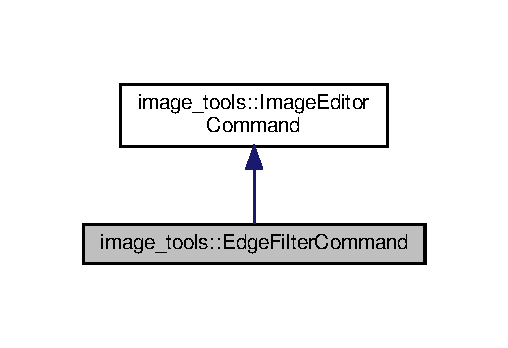
\includegraphics[width=244pt]{classimage__tools_1_1EdgeFilterCommand__inherit__graph}
\end{center}
\end{figure}


Collaboration diagram for image\+\_\+tools\+:\+:Edge\+Filter\+Command\+:
\nopagebreak
\begin{figure}[H]
\begin{center}
\leavevmode
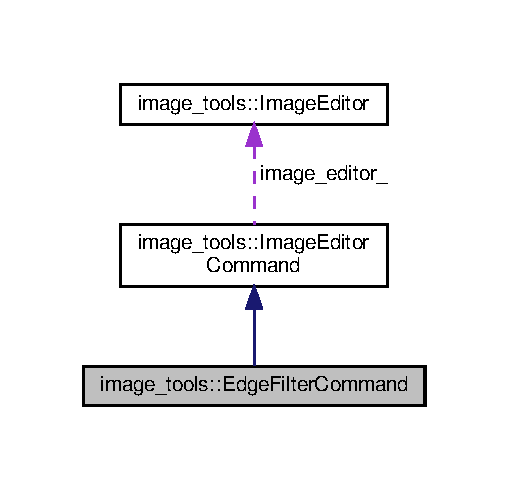
\includegraphics[width=244pt]{classimage__tools_1_1EdgeFilterCommand__coll__graph}
\end{center}
\end{figure}
\subsection*{Public Member Functions}
\begin{DoxyCompactItemize}
\item 
\mbox{\Hypertarget{classimage__tools_1_1EdgeFilterCommand_ad0b9f05e02602d079c5864705465adfe}\label{classimage__tools_1_1EdgeFilterCommand_ad0b9f05e02602d079c5864705465adfe}} 
{\bfseries Edge\+Filter\+Command} (\hyperlink{classimage__tools_1_1ImageEditor}{Image\+Editor} $\ast$image\+\_\+editor)
\item 
\mbox{\Hypertarget{classimage__tools_1_1EdgeFilterCommand_ac2889f9d8ba5307498239d954db5e632}\label{classimage__tools_1_1EdgeFilterCommand_ac2889f9d8ba5307498239d954db5e632}} 
void {\bfseries Execute} () override
\end{DoxyCompactItemize}
\subsection*{Additional Inherited Members}


\subsection{Detailed Description}
Specific command for executing an edge detection filter. 

The documentation for this class was generated from the following files\+:\begin{DoxyCompactItemize}
\item 
src/mia/image\+\_\+editor\+\_\+commands.\+h\item 
src/mia/image\+\_\+editor\+\_\+commands.\+cc\end{DoxyCompactItemize}

\hypertarget{classimage__tools_1_1EndStrokeCommand}{}\section{image\+\_\+tools\+:\+:End\+Stroke\+Command Class Reference}
\label{classimage__tools_1_1EndStrokeCommand}\index{image\+\_\+tools\+::\+End\+Stroke\+Command@{image\+\_\+tools\+::\+End\+Stroke\+Command}}


{\ttfamily \#include $<$image\+\_\+editor\+\_\+commands.\+h$>$}



Inheritance diagram for image\+\_\+tools\+:\+:End\+Stroke\+Command\+:
\nopagebreak
\begin{figure}[H]
\begin{center}
\leavevmode
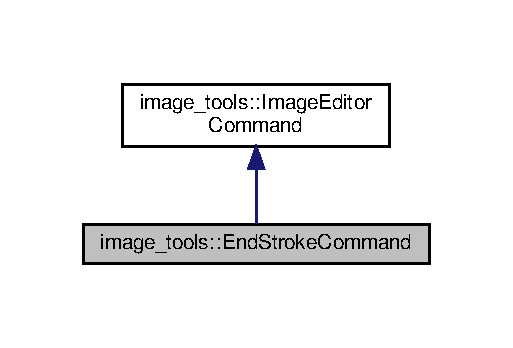
\includegraphics[width=246pt]{classimage__tools_1_1EndStrokeCommand__inherit__graph}
\end{center}
\end{figure}


Collaboration diagram for image\+\_\+tools\+:\+:End\+Stroke\+Command\+:
\nopagebreak
\begin{figure}[H]
\begin{center}
\leavevmode
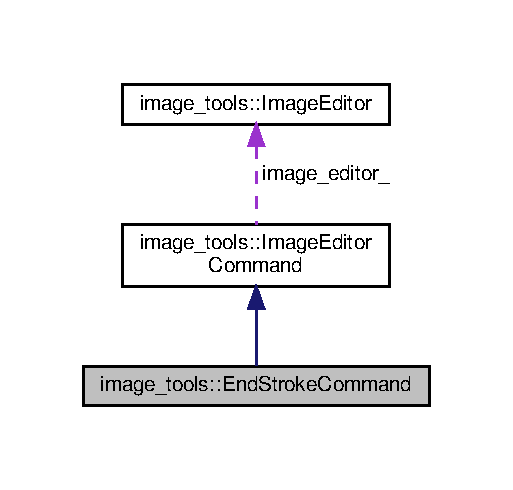
\includegraphics[width=246pt]{classimage__tools_1_1EndStrokeCommand__coll__graph}
\end{center}
\end{figure}
\subsection*{Public Member Functions}
\begin{DoxyCompactItemize}
\item 
\mbox{\Hypertarget{classimage__tools_1_1EndStrokeCommand_ab70066942dc6862754fd7530330f6325}\label{classimage__tools_1_1EndStrokeCommand_ab70066942dc6862754fd7530330f6325}} 
{\bfseries End\+Stroke\+Command} (\hyperlink{classimage__tools_1_1ImageEditor}{Image\+Editor} $\ast$image\+\_\+editor, int x, int y)
\item 
\mbox{\Hypertarget{classimage__tools_1_1EndStrokeCommand_a2bc57e28b0060b88b38cc6fb84b9711f}\label{classimage__tools_1_1EndStrokeCommand_a2bc57e28b0060b88b38cc6fb84b9711f}} 
void {\bfseries Execute} () override
\end{DoxyCompactItemize}
\subsection*{Additional Inherited Members}


\subsection{Detailed Description}
Specific command for ending the stroke. 

The documentation for this class was generated from the following files\+:\begin{DoxyCompactItemize}
\item 
src/mia/image\+\_\+editor\+\_\+commands.\+h\item 
src/mia/image\+\_\+editor\+\_\+commands.\+cc\end{DoxyCompactItemize}

\hypertarget{classimage__tools_1_1Filter}{}\section{image\+\_\+tools\+:\+:Filter Class Reference}
\label{classimage__tools_1_1Filter}\index{image\+\_\+tools\+::\+Filter@{image\+\_\+tools\+::\+Filter}}


Serves as the parent class to implement all filters. Modifies an image by changing each pixel value within the image.  




{\ttfamily \#include $<$filter.\+h$>$}



Inheritance diagram for image\+\_\+tools\+:\+:Filter\+:
\nopagebreak
\begin{figure}[H]
\begin{center}
\leavevmode
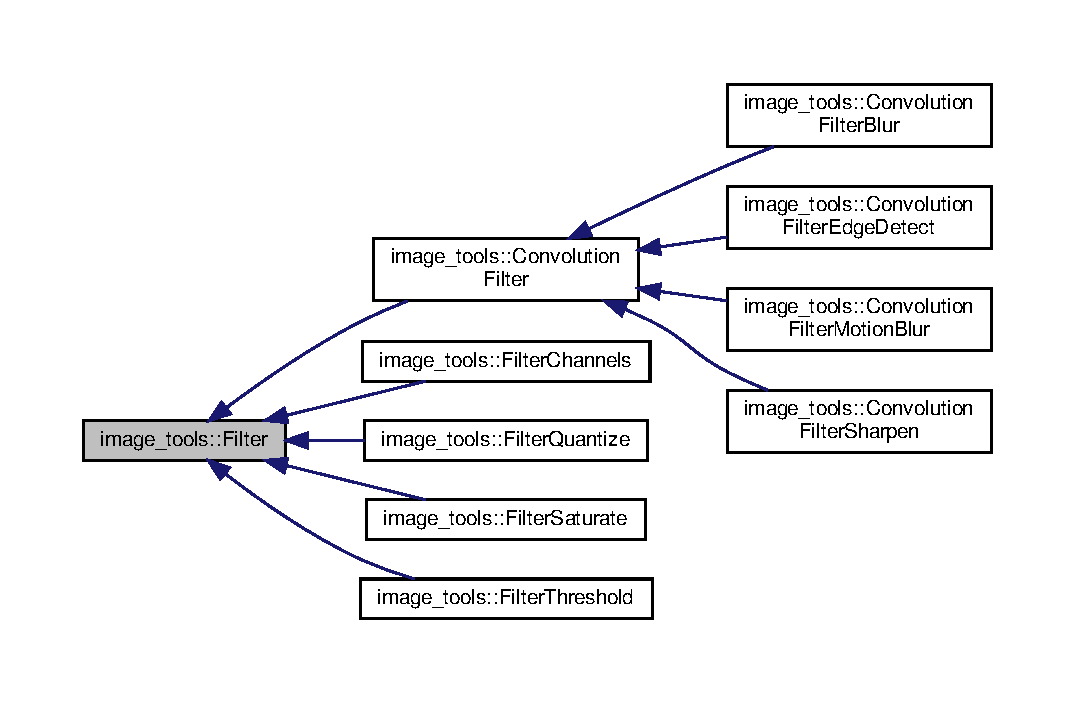
\includegraphics[width=350pt]{classimage__tools_1_1Filter__inherit__graph}
\end{center}
\end{figure}
\subsection*{Public Member Functions}
\begin{DoxyCompactItemize}
\item 
\mbox{\Hypertarget{classimage__tools_1_1Filter_af621f9c2221e0a5310322413f0adfca5}\label{classimage__tools_1_1Filter_af621f9c2221e0a5310322413f0adfca5}} 
virtual void {\bfseries Setup\+Filter} ()
\item 
\mbox{\Hypertarget{classimage__tools_1_1Filter_abb92717e3b5d762720d8a80f6b10dd5d}\label{classimage__tools_1_1Filter_abb92717e3b5d762720d8a80f6b10dd5d}} 
virtual void \hyperlink{classimage__tools_1_1Filter_abb92717e3b5d762720d8a80f6b10dd5d}{Cleanup\+Filter} ()
\begin{DoxyCompactList}\small\item\em Deletes pointer. \end{DoxyCompactList}\item 
virtual bool \hyperlink{classimage__tools_1_1Filter_abb21c6ce1f09a4ce4fbd38255c44d281}{can\+\_\+copy\+\_\+in\+\_\+place} ()
\item 
virtual \hyperlink{classimage__tools_1_1ColorData}{Color\+Data} \hyperlink{classimage__tools_1_1Filter_a68d38fa12b87e20b81090cb380c0a307}{Calculate\+Filtered\+Pixel} (\hyperlink{classimage__tools_1_1PixelBuffer}{Pixel\+Buffer} $\ast$buffer, int x, int y)
\item 
\mbox{\Hypertarget{classimage__tools_1_1Filter_a2e546a29d5c7dc1d7fff50d0f06b4c2b}\label{classimage__tools_1_1Filter_a2e546a29d5c7dc1d7fff50d0f06b4c2b}} 
void {\bfseries Apply\+To\+Buffer} (\hyperlink{classimage__tools_1_1PixelBuffer}{Pixel\+Buffer} $\ast$buffer)
\end{DoxyCompactItemize}


\subsection{Detailed Description}
Serves as the parent class to implement all filters. Modifies an image by changing each pixel value within the image. 

\subsection{Member Function Documentation}
\mbox{\Hypertarget{classimage__tools_1_1Filter_a68d38fa12b87e20b81090cb380c0a307}\label{classimage__tools_1_1Filter_a68d38fa12b87e20b81090cb380c0a307}} 
\index{image\+\_\+tools\+::\+Filter@{image\+\_\+tools\+::\+Filter}!Calculate\+Filtered\+Pixel@{Calculate\+Filtered\+Pixel}}
\index{Calculate\+Filtered\+Pixel@{Calculate\+Filtered\+Pixel}!image\+\_\+tools\+::\+Filter@{image\+\_\+tools\+::\+Filter}}
\subsubsection{\texorpdfstring{Calculate\+Filtered\+Pixel()}{CalculateFilteredPixel()}}
{\footnotesize\ttfamily \hyperlink{classimage__tools_1_1ColorData}{Color\+Data} image\+\_\+tools\+::\+Filter\+::\+Calculate\+Filtered\+Pixel (\begin{DoxyParamCaption}\item[{\hyperlink{classimage__tools_1_1PixelBuffer}{Pixel\+Buffer} $\ast$}]{buffer,  }\item[{int}]{x,  }\item[{int}]{y }\end{DoxyParamCaption})\hspace{0.3cm}{\ttfamily [virtual]}}

Applies a filter by looping through each pixel in an image and modifying that pixel. 

Reimplemented in \hyperlink{classimage__tools_1_1ConvolutionFilter_a2d35a2e2a2d1303d0a6824b16406d97b}{image\+\_\+tools\+::\+Convolution\+Filter}, \hyperlink{classimage__tools_1_1FilterQuantize_a312afa1aa4af5c58b7ec6d5faad0a176}{image\+\_\+tools\+::\+Filter\+Quantize}, \hyperlink{classimage__tools_1_1FilterSaturate_a86ab1b87e52a5f9b5c8642531ed7fdc6}{image\+\_\+tools\+::\+Filter\+Saturate}, \hyperlink{classimage__tools_1_1FilterThreshold_a905065fd47d7228b11354795e487b2c6}{image\+\_\+tools\+::\+Filter\+Threshold}, and \hyperlink{classimage__tools_1_1FilterChannels_a99af7bdf46f4d606fae4baa793025836}{image\+\_\+tools\+::\+Filter\+Channels}.

\mbox{\Hypertarget{classimage__tools_1_1Filter_abb21c6ce1f09a4ce4fbd38255c44d281}\label{classimage__tools_1_1Filter_abb21c6ce1f09a4ce4fbd38255c44d281}} 
\index{image\+\_\+tools\+::\+Filter@{image\+\_\+tools\+::\+Filter}!can\+\_\+copy\+\_\+in\+\_\+place@{can\+\_\+copy\+\_\+in\+\_\+place}}
\index{can\+\_\+copy\+\_\+in\+\_\+place@{can\+\_\+copy\+\_\+in\+\_\+place}!image\+\_\+tools\+::\+Filter@{image\+\_\+tools\+::\+Filter}}
\subsubsection{\texorpdfstring{can\+\_\+copy\+\_\+in\+\_\+place()}{can\_copy\_in\_place()}}
{\footnotesize\ttfamily bool image\+\_\+tools\+::\+Filter\+::can\+\_\+copy\+\_\+in\+\_\+place (\begin{DoxyParamCaption}{ }\end{DoxyParamCaption})\hspace{0.3cm}{\ttfamily [virtual]}}

Simple filters (\hyperlink{classimage__tools_1_1FilterChannels}{Filter\+Channels}, \hyperlink{classimage__tools_1_1FilterQuantize}{Filter\+Quantize}, \hyperlink{classimage__tools_1_1FilterSaturate}{Filter\+Saturate}, and \hyperlink{classimage__tools_1_1FilterThreshold}{Filter\+Threshold}) can be copied in place, whereas convolution filters (\hyperlink{classimage__tools_1_1ConvolutionFilterBlur}{Convolution\+Filter\+Blur}, \hyperlink{classimage__tools_1_1ConvolutionFilterEdgeDetect}{Convolution\+Filter\+Edge\+Detect}, \hyperlink{classimage__tools_1_1ConvolutionFilterMotionBlur}{Convolution\+Filter\+Motion\+Blur}, and \hyperlink{classimage__tools_1_1ConvolutionFilterSharpen}{Convolution\+Filter\+Sharpen} ) cannot. 

Reimplemented in \hyperlink{classimage__tools_1_1ConvolutionFilter_aef03779d74d96173880d93d06c7bd6b6}{image\+\_\+tools\+::\+Convolution\+Filter}.



The documentation for this class was generated from the following files\+:\begin{DoxyCompactItemize}
\item 
src/imagetools/filter.\+h\item 
src/imagetools/filter.\+cc\end{DoxyCompactItemize}

\hypertarget{classimage__tools_1_1FilterChannels}{}\section{image\+\_\+tools\+:\+:Filter\+Channels Class Reference}
\label{classimage__tools_1_1FilterChannels}\index{image\+\_\+tools\+::\+Filter\+Channels@{image\+\_\+tools\+::\+Filter\+Channels}}


Implements a filter by adjusting the red, green, blue values of each pixel.  




{\ttfamily \#include $<$filter\+\_\+channels.\+h$>$}



Inheritance diagram for image\+\_\+tools\+:\+:Filter\+Channels\+:
\nopagebreak
\begin{figure}[H]
\begin{center}
\leavevmode
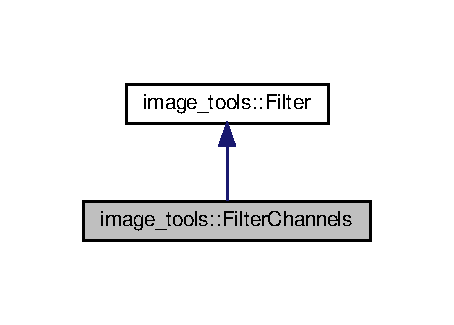
\includegraphics[width=218pt]{classimage__tools_1_1FilterChannels__inherit__graph}
\end{center}
\end{figure}


Collaboration diagram for image\+\_\+tools\+:\+:Filter\+Channels\+:
\nopagebreak
\begin{figure}[H]
\begin{center}
\leavevmode
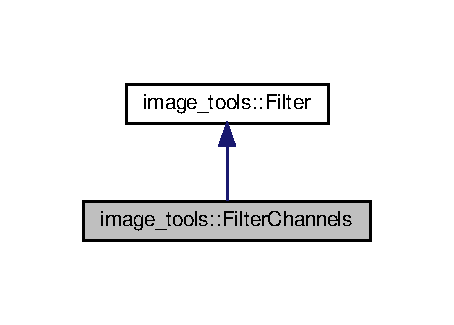
\includegraphics[width=218pt]{classimage__tools_1_1FilterChannels__coll__graph}
\end{center}
\end{figure}
\subsection*{Public Member Functions}
\begin{DoxyCompactItemize}
\item 
\mbox{\Hypertarget{classimage__tools_1_1FilterChannels_aabe05d8cef0727cd96baa22d18b2e50e}\label{classimage__tools_1_1FilterChannels_aabe05d8cef0727cd96baa22d18b2e50e}} 
\hyperlink{classimage__tools_1_1FilterChannels_aabe05d8cef0727cd96baa22d18b2e50e}{Filter\+Channels} ()
\begin{DoxyCompactList}\small\item\em Defaults to r=0.\+5, g=0.\+5, and b=0.\+5. \end{DoxyCompactList}\item 
\hyperlink{classimage__tools_1_1ColorData}{Color\+Data} \hyperlink{classimage__tools_1_1FilterChannels_a99af7bdf46f4d606fae4baa793025836}{Calculate\+Filtered\+Pixel} (\hyperlink{classimage__tools_1_1PixelBuffer}{Pixel\+Buffer} $\ast$buffer, int x, int y) override
\item 
\mbox{\Hypertarget{classimage__tools_1_1FilterChannels_a2c48ab1acde424eee37af26745f9ce29}\label{classimage__tools_1_1FilterChannels_a2c48ab1acde424eee37af26745f9ce29}} 
void {\bfseries Set\+Values} (float r, float g, float b)
\end{DoxyCompactItemize}


\subsection{Detailed Description}
Implements a filter by adjusting the red, green, blue values of each pixel. 

\subsection{Member Function Documentation}
\mbox{\Hypertarget{classimage__tools_1_1FilterChannels_a99af7bdf46f4d606fae4baa793025836}\label{classimage__tools_1_1FilterChannels_a99af7bdf46f4d606fae4baa793025836}} 
\index{image\+\_\+tools\+::\+Filter\+Channels@{image\+\_\+tools\+::\+Filter\+Channels}!Calculate\+Filtered\+Pixel@{Calculate\+Filtered\+Pixel}}
\index{Calculate\+Filtered\+Pixel@{Calculate\+Filtered\+Pixel}!image\+\_\+tools\+::\+Filter\+Channels@{image\+\_\+tools\+::\+Filter\+Channels}}
\subsubsection{\texorpdfstring{Calculate\+Filtered\+Pixel()}{CalculateFilteredPixel()}}
{\footnotesize\ttfamily \hyperlink{classimage__tools_1_1ColorData}{Color\+Data} image\+\_\+tools\+::\+Filter\+Channels\+::\+Calculate\+Filtered\+Pixel (\begin{DoxyParamCaption}\item[{\hyperlink{classimage__tools_1_1PixelBuffer}{Pixel\+Buffer} $\ast$}]{buffer,  }\item[{int}]{x,  }\item[{int}]{y }\end{DoxyParamCaption})\hspace{0.3cm}{\ttfamily [override]}, {\ttfamily [virtual]}}

Applies a filter by looping through each pixel in an image and modifying that pixel. 

Reimplemented from \hyperlink{classimage__tools_1_1Filter_a68d38fa12b87e20b81090cb380c0a307}{image\+\_\+tools\+::\+Filter}.



The documentation for this class was generated from the following files\+:\begin{DoxyCompactItemize}
\item 
src/imagetools/filter\+\_\+channels.\+h\item 
src/imagetools/filter\+\_\+channels.\+cc\end{DoxyCompactItemize}

\hypertarget{classimage__tools_1_1FilterQuantize}{}\section{image\+\_\+tools\+:\+:Filter\+Quantize Class Reference}
\label{classimage__tools_1_1FilterQuantize}\index{image\+\_\+tools\+::\+Filter\+Quantize@{image\+\_\+tools\+::\+Filter\+Quantize}}


Implements a filter by reducing the number of colors in the image via a binning method. Each color channel is modified by placing it into the closest bin.  




{\ttfamily \#include $<$filter\+\_\+quantize.\+h$>$}



Inheritance diagram for image\+\_\+tools\+:\+:Filter\+Quantize\+:
\nopagebreak
\begin{figure}[H]
\begin{center}
\leavevmode
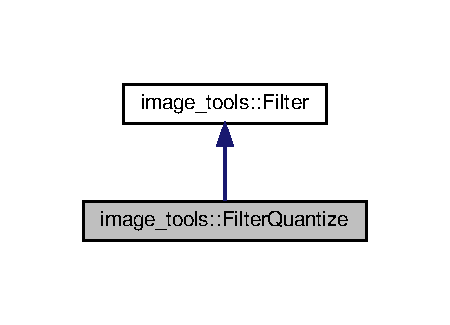
\includegraphics[width=216pt]{classimage__tools_1_1FilterQuantize__inherit__graph}
\end{center}
\end{figure}


Collaboration diagram for image\+\_\+tools\+:\+:Filter\+Quantize\+:
\nopagebreak
\begin{figure}[H]
\begin{center}
\leavevmode
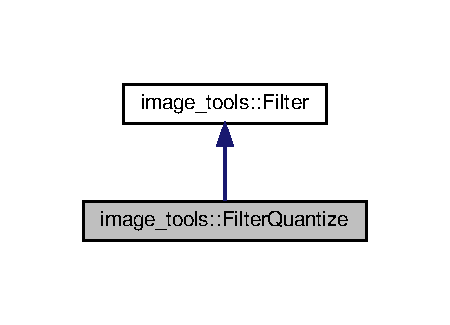
\includegraphics[width=216pt]{classimage__tools_1_1FilterQuantize__coll__graph}
\end{center}
\end{figure}
\subsection*{Public Member Functions}
\begin{DoxyCompactItemize}
\item 
\mbox{\Hypertarget{classimage__tools_1_1FilterQuantize_aeba7a9d7a4260f74fdff4a550181a8e1}\label{classimage__tools_1_1FilterQuantize_aeba7a9d7a4260f74fdff4a550181a8e1}} 
\hyperlink{classimage__tools_1_1FilterQuantize_aeba7a9d7a4260f74fdff4a550181a8e1}{Filter\+Quantize} ()
\begin{DoxyCompactList}\small\item\em Defaults to bin\+\_\+val=1. \end{DoxyCompactList}\item 
\hyperlink{classimage__tools_1_1ColorData}{Color\+Data} \hyperlink{classimage__tools_1_1FilterQuantize_a312afa1aa4af5c58b7ec6d5faad0a176}{Calculate\+Filtered\+Pixel} (\hyperlink{classimage__tools_1_1PixelBuffer}{Pixel\+Buffer} $\ast$buffer, int x, int y) override
\item 
\mbox{\Hypertarget{classimage__tools_1_1FilterQuantize_a8be8db0926f5701615320882f60f9d45}\label{classimage__tools_1_1FilterQuantize_a8be8db0926f5701615320882f60f9d45}} 
void {\bfseries Set\+Value} (int bin\+\_\+val)
\end{DoxyCompactItemize}


\subsection{Detailed Description}
Implements a filter by reducing the number of colors in the image via a binning method. Each color channel is modified by placing it into the closest bin. 

\subsection{Member Function Documentation}
\mbox{\Hypertarget{classimage__tools_1_1FilterQuantize_a312afa1aa4af5c58b7ec6d5faad0a176}\label{classimage__tools_1_1FilterQuantize_a312afa1aa4af5c58b7ec6d5faad0a176}} 
\index{image\+\_\+tools\+::\+Filter\+Quantize@{image\+\_\+tools\+::\+Filter\+Quantize}!Calculate\+Filtered\+Pixel@{Calculate\+Filtered\+Pixel}}
\index{Calculate\+Filtered\+Pixel@{Calculate\+Filtered\+Pixel}!image\+\_\+tools\+::\+Filter\+Quantize@{image\+\_\+tools\+::\+Filter\+Quantize}}
\subsubsection{\texorpdfstring{Calculate\+Filtered\+Pixel()}{CalculateFilteredPixel()}}
{\footnotesize\ttfamily \hyperlink{classimage__tools_1_1ColorData}{Color\+Data} image\+\_\+tools\+::\+Filter\+Quantize\+::\+Calculate\+Filtered\+Pixel (\begin{DoxyParamCaption}\item[{\hyperlink{classimage__tools_1_1PixelBuffer}{Pixel\+Buffer} $\ast$}]{buffer,  }\item[{int}]{x,  }\item[{int}]{y }\end{DoxyParamCaption})\hspace{0.3cm}{\ttfamily [override]}, {\ttfamily [virtual]}}

Applies a filter by looping through each pixel in an image and modifying that pixel. 

Reimplemented from \hyperlink{classimage__tools_1_1Filter_a68d38fa12b87e20b81090cb380c0a307}{image\+\_\+tools\+::\+Filter}.



The documentation for this class was generated from the following files\+:\begin{DoxyCompactItemize}
\item 
src/imagetools/filter\+\_\+quantize.\+h\item 
src/imagetools/filter\+\_\+quantize.\+cc\end{DoxyCompactItemize}

\hypertarget{classimage__tools_1_1FilterSaturate}{}\section{image\+\_\+tools\+:\+:Filter\+Saturate Class Reference}
\label{classimage__tools_1_1FilterSaturate}\index{image\+\_\+tools\+::\+Filter\+Saturate@{image\+\_\+tools\+::\+Filter\+Saturate}}


Implements a filter by increasing or decreasing the intensity of an image\textquotesingle{}s colors.  




{\ttfamily \#include $<$filter\+\_\+saturate.\+h$>$}



Inheritance diagram for image\+\_\+tools\+:\+:Filter\+Saturate\+:
\nopagebreak
\begin{figure}[H]
\begin{center}
\leavevmode
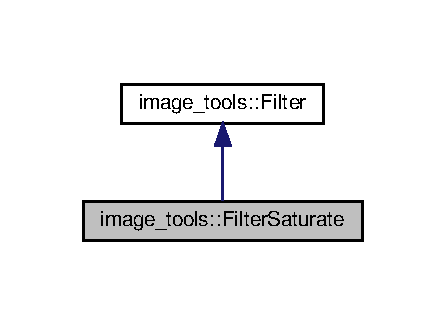
\includegraphics[width=214pt]{classimage__tools_1_1FilterSaturate__inherit__graph}
\end{center}
\end{figure}


Collaboration diagram for image\+\_\+tools\+:\+:Filter\+Saturate\+:
\nopagebreak
\begin{figure}[H]
\begin{center}
\leavevmode
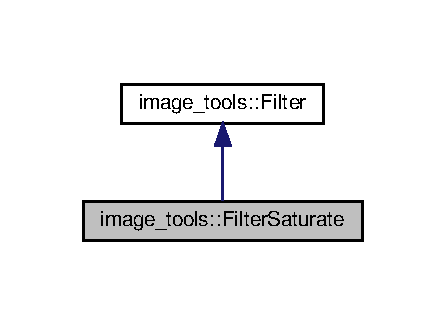
\includegraphics[width=214pt]{classimage__tools_1_1FilterSaturate__coll__graph}
\end{center}
\end{figure}
\subsection*{Public Member Functions}
\begin{DoxyCompactItemize}
\item 
\mbox{\Hypertarget{classimage__tools_1_1FilterSaturate_adb9cbb52d0cbcbb301eebcbced82bd3d}\label{classimage__tools_1_1FilterSaturate_adb9cbb52d0cbcbb301eebcbced82bd3d}} 
\hyperlink{classimage__tools_1_1FilterSaturate_adb9cbb52d0cbcbb301eebcbced82bd3d}{Filter\+Saturate} ()
\begin{DoxyCompactList}\small\item\em Defaults to sat\+\_\+value=0.\+5. \end{DoxyCompactList}\item 
\hyperlink{classimage__tools_1_1ColorData}{Color\+Data} \hyperlink{classimage__tools_1_1FilterSaturate_a86ab1b87e52a5f9b5c8642531ed7fdc6}{Calculate\+Filtered\+Pixel} (\hyperlink{classimage__tools_1_1PixelBuffer}{Pixel\+Buffer} $\ast$buffer, int x, int y) override
\item 
\mbox{\Hypertarget{classimage__tools_1_1FilterSaturate_a31182a6d8f384ac6d73c8367d1776535}\label{classimage__tools_1_1FilterSaturate_a31182a6d8f384ac6d73c8367d1776535}} 
void {\bfseries Set\+Value} (float sat\+\_\+val)
\end{DoxyCompactItemize}


\subsection{Detailed Description}
Implements a filter by increasing or decreasing the intensity of an image\textquotesingle{}s colors. 

\subsection{Member Function Documentation}
\mbox{\Hypertarget{classimage__tools_1_1FilterSaturate_a86ab1b87e52a5f9b5c8642531ed7fdc6}\label{classimage__tools_1_1FilterSaturate_a86ab1b87e52a5f9b5c8642531ed7fdc6}} 
\index{image\+\_\+tools\+::\+Filter\+Saturate@{image\+\_\+tools\+::\+Filter\+Saturate}!Calculate\+Filtered\+Pixel@{Calculate\+Filtered\+Pixel}}
\index{Calculate\+Filtered\+Pixel@{Calculate\+Filtered\+Pixel}!image\+\_\+tools\+::\+Filter\+Saturate@{image\+\_\+tools\+::\+Filter\+Saturate}}
\subsubsection{\texorpdfstring{Calculate\+Filtered\+Pixel()}{CalculateFilteredPixel()}}
{\footnotesize\ttfamily \hyperlink{classimage__tools_1_1ColorData}{Color\+Data} image\+\_\+tools\+::\+Filter\+Saturate\+::\+Calculate\+Filtered\+Pixel (\begin{DoxyParamCaption}\item[{\hyperlink{classimage__tools_1_1PixelBuffer}{Pixel\+Buffer} $\ast$}]{buffer,  }\item[{int}]{x,  }\item[{int}]{y }\end{DoxyParamCaption})\hspace{0.3cm}{\ttfamily [override]}, {\ttfamily [virtual]}}

Applies a filter by looping through each pixel in an image and modifying that pixel. 

Reimplemented from \hyperlink{classimage__tools_1_1Filter_a68d38fa12b87e20b81090cb380c0a307}{image\+\_\+tools\+::\+Filter}.



The documentation for this class was generated from the following files\+:\begin{DoxyCompactItemize}
\item 
src/imagetools/filter\+\_\+saturate.\+h\item 
src/imagetools/filter\+\_\+saturate.\+cc\end{DoxyCompactItemize}

\hypertarget{classimage__tools_1_1FilterThreshold}{}\section{image\+\_\+tools\+:\+:Filter\+Threshold Class Reference}
\label{classimage__tools_1_1FilterThreshold}\index{image\+\_\+tools\+::\+Filter\+Threshold@{image\+\_\+tools\+::\+Filter\+Threshold}}


Implements a filter by rounding an image\textquotesingle{}s R\+GB value up to 1.\+0 (white) if it\textquotesingle{}s pixel value is greater than the threshold input or down to 0.\+0 (black) if it\textquotesingle{}s pixel value is lower than the threshold input.  




{\ttfamily \#include $<$filter\+\_\+threshold.\+h$>$}



Inheritance diagram for image\+\_\+tools\+:\+:Filter\+Threshold\+:
\nopagebreak
\begin{figure}[H]
\begin{center}
\leavevmode
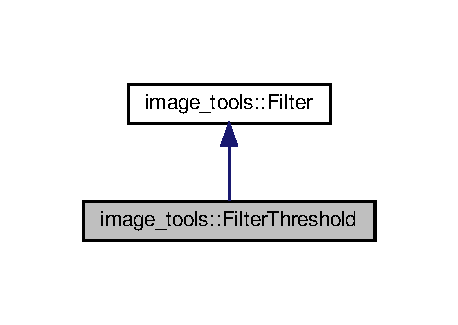
\includegraphics[width=220pt]{classimage__tools_1_1FilterThreshold__inherit__graph}
\end{center}
\end{figure}


Collaboration diagram for image\+\_\+tools\+:\+:Filter\+Threshold\+:
\nopagebreak
\begin{figure}[H]
\begin{center}
\leavevmode
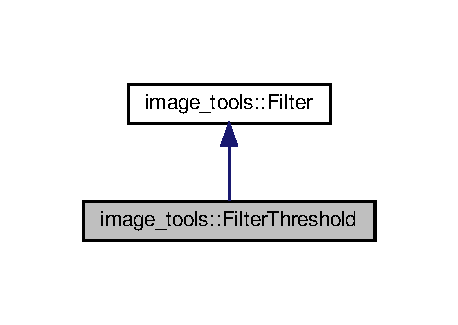
\includegraphics[width=220pt]{classimage__tools_1_1FilterThreshold__coll__graph}
\end{center}
\end{figure}
\subsection*{Public Member Functions}
\begin{DoxyCompactItemize}
\item 
\mbox{\Hypertarget{classimage__tools_1_1FilterThreshold_a10675d611d33cdead5ddecfaa3b8494c}\label{classimage__tools_1_1FilterThreshold_a10675d611d33cdead5ddecfaa3b8494c}} 
\hyperlink{classimage__tools_1_1FilterThreshold_a10675d611d33cdead5ddecfaa3b8494c}{Filter\+Threshold} ()
\begin{DoxyCompactList}\small\item\em Defaults to threshold\+\_\+val=0.\+5. \end{DoxyCompactList}\item 
\hyperlink{classimage__tools_1_1ColorData}{Color\+Data} \hyperlink{classimage__tools_1_1FilterThreshold_a905065fd47d7228b11354795e487b2c6}{Calculate\+Filtered\+Pixel} (\hyperlink{classimage__tools_1_1PixelBuffer}{Pixel\+Buffer} $\ast$buffer, int x, int y) override
\item 
\mbox{\Hypertarget{classimage__tools_1_1FilterThreshold_a1c939ef99b6370970ce6ca0227d66ad6}\label{classimage__tools_1_1FilterThreshold_a1c939ef99b6370970ce6ca0227d66ad6}} 
void {\bfseries Set\+Value} (float threshold\+\_\+val)
\end{DoxyCompactItemize}


\subsection{Detailed Description}
Implements a filter by rounding an image\textquotesingle{}s R\+GB value up to 1.\+0 (white) if it\textquotesingle{}s pixel value is greater than the threshold input or down to 0.\+0 (black) if it\textquotesingle{}s pixel value is lower than the threshold input. 

\subsection{Member Function Documentation}
\mbox{\Hypertarget{classimage__tools_1_1FilterThreshold_a905065fd47d7228b11354795e487b2c6}\label{classimage__tools_1_1FilterThreshold_a905065fd47d7228b11354795e487b2c6}} 
\index{image\+\_\+tools\+::\+Filter\+Threshold@{image\+\_\+tools\+::\+Filter\+Threshold}!Calculate\+Filtered\+Pixel@{Calculate\+Filtered\+Pixel}}
\index{Calculate\+Filtered\+Pixel@{Calculate\+Filtered\+Pixel}!image\+\_\+tools\+::\+Filter\+Threshold@{image\+\_\+tools\+::\+Filter\+Threshold}}
\subsubsection{\texorpdfstring{Calculate\+Filtered\+Pixel()}{CalculateFilteredPixel()}}
{\footnotesize\ttfamily \hyperlink{classimage__tools_1_1ColorData}{Color\+Data} image\+\_\+tools\+::\+Filter\+Threshold\+::\+Calculate\+Filtered\+Pixel (\begin{DoxyParamCaption}\item[{\hyperlink{classimage__tools_1_1PixelBuffer}{Pixel\+Buffer} $\ast$}]{buffer,  }\item[{int}]{x,  }\item[{int}]{y }\end{DoxyParamCaption})\hspace{0.3cm}{\ttfamily [override]}, {\ttfamily [virtual]}}

Applies a filter by looping through each pixel in an image and modifying that pixel. 

Reimplemented from \hyperlink{classimage__tools_1_1Filter_a68d38fa12b87e20b81090cb380c0a307}{image\+\_\+tools\+::\+Filter}.



The documentation for this class was generated from the following files\+:\begin{DoxyCompactItemize}
\item 
src/imagetools/filter\+\_\+threshold.\+h\item 
src/imagetools/filter\+\_\+threshold.\+cc\end{DoxyCompactItemize}

\hypertarget{classimage__tools_1_1FlashPhotoApp}{}\section{image\+\_\+tools\+:\+:Flash\+Photo\+App Class Reference}
\label{classimage__tools_1_1FlashPhotoApp}\index{image\+\_\+tools\+::\+Flash\+Photo\+App@{image\+\_\+tools\+::\+Flash\+Photo\+App}}


The Flash\+Photo G\+UI. This class creates a graphics window to display the current \hyperlink{classimage__tools_1_1PixelBuffer}{Pixel\+Buffer} and a graphical user interface to interact with it using Tools and Filters.  




{\ttfamily \#include $<$flashphoto\+\_\+app.\+h$>$}



Inheritance diagram for image\+\_\+tools\+:\+:Flash\+Photo\+App\+:
\nopagebreak
\begin{figure}[H]
\begin{center}
\leavevmode
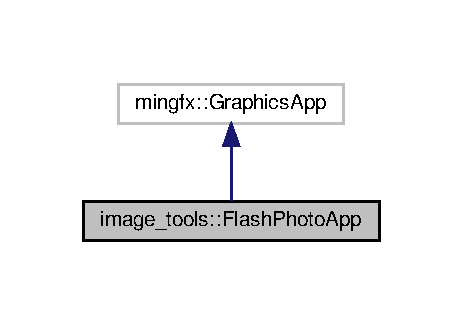
\includegraphics[width=222pt]{classimage__tools_1_1FlashPhotoApp__inherit__graph}
\end{center}
\end{figure}


Collaboration diagram for image\+\_\+tools\+:\+:Flash\+Photo\+App\+:
\nopagebreak
\begin{figure}[H]
\begin{center}
\leavevmode
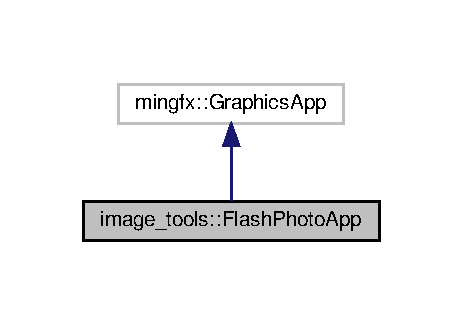
\includegraphics[width=222pt]{classimage__tools_1_1FlashPhotoApp__coll__graph}
\end{center}
\end{figure}
\subsection*{Public Member Functions}
\begin{DoxyCompactItemize}
\item 
\mbox{\Hypertarget{classimage__tools_1_1FlashPhotoApp_ae5fac55fc6210eb08bde89343170bfe0}\label{classimage__tools_1_1FlashPhotoApp_ae5fac55fc6210eb08bde89343170bfe0}} 
{\bfseries Flash\+Photo\+App} (int width, int height, const \hyperlink{classimage__tools_1_1ColorData}{Color\+Data} \&background\+\_\+color)
\item 
void \hyperlink{classimage__tools_1_1FlashPhotoApp_aba314de10932cab1acbf34debbbb9776}{On\+Mouse\+Move} (const mingfx\+::\+Point2 \&pos, const mingfx\+::\+Vector2 \&delta) override
\item 
void \hyperlink{classimage__tools_1_1FlashPhotoApp_af26aeb5420b9f123fba9330abc3ff907}{On\+Left\+Mouse\+Down} (const mingfx\+::\+Point2 \&pos) override
\item 
void \hyperlink{classimage__tools_1_1FlashPhotoApp_a900752c3758c9a92619a24b7c3e351e8}{On\+Left\+Mouse\+Drag} (const mingfx\+::\+Point2 \&pos, const mingfx\+::\+Vector2 \&delta) override
\item 
void \hyperlink{classimage__tools_1_1FlashPhotoApp_a63ce75bf69e79b7db32f07f0cd9c50b7}{On\+Left\+Mouse\+Up} (const mingfx\+::\+Point2 \&pos) override
\item 
void \hyperlink{classimage__tools_1_1FlashPhotoApp_afab3ded368aee035c7c229226048479a}{On\+Window\+Resize} (int new\+\_\+width, int new\+\_\+height) override
\item 
void \hyperlink{classimage__tools_1_1FlashPhotoApp_af69350137d0f9f7501853d23a72c7f4e}{Update\+Simulation} (double dt) override
\item 
void \hyperlink{classimage__tools_1_1FlashPhotoApp_a58a876833577928a4a361e9b14a03680}{Init\+Nano\+G\+UI} () override
\item 
void \hyperlink{classimage__tools_1_1FlashPhotoApp_a8824007bb6ed253f1b5a37d458ff2371}{Init\+Open\+GL} () override
\item 
void \hyperlink{classimage__tools_1_1FlashPhotoApp_abda3c07c67a29eba47e341bdf0223e7a}{Draw\+Using\+Nano\+VG} (N\+V\+Gcontext $\ast$ctx) override
\item 
void \hyperlink{classimage__tools_1_1FlashPhotoApp_a58e520556daa81224cb0a76a3fca9b78}{Draw\+Using\+Open\+GL} () override
\item 
void \hyperlink{classimage__tools_1_1FlashPhotoApp_aee942a00db0ff47ed36f4a78bf308482}{Load\+From\+File} (const std\+::string \&filename)
\item 
void \hyperlink{classimage__tools_1_1FlashPhotoApp_a292e1e58a4848cbf055def1ad0acd79a}{Save\+To\+File} (const std\+::string \&filename)
\item 
\mbox{\Hypertarget{classimage__tools_1_1FlashPhotoApp_a4e9f1d7e08fbb87ad67027c4021066c8}\label{classimage__tools_1_1FlashPhotoApp_a4e9f1d7e08fbb87ad67027c4021066c8}} 
\hyperlink{classimage__tools_1_1Tool}{Tool} $\ast$ {\bfseries Get\+Tool\+By\+Name} (const std\+::string \&name)
\item 
void \hyperlink{classimage__tools_1_1FlashPhotoApp_ab40b6ecc2ba4caa35b8e18f091b67253}{Start\+Stroke} (const std\+::string \&tool\+\_\+name, const \hyperlink{classimage__tools_1_1ColorData}{Color\+Data} \&color, float radius, int x, int y)
\item 
void \hyperlink{classimage__tools_1_1FlashPhotoApp_a1ede0fe70602cbe2d50a3123eda8a937}{Add\+To\+Stroke} (int x, int y)
\item 
void \hyperlink{classimage__tools_1_1FlashPhotoApp_a34682088e7957ea5e5adf084d2a292a8}{End\+Stroke} (int x, int y)
\item 
void \hyperlink{classimage__tools_1_1FlashPhotoApp_ab9de628d295f2ce1ea869767cb918a2d}{Apply\+Blur\+Filter} (float radius)
\begin{DoxyCompactList}\small\item\em Four possible motion blur directions are supported. \end{DoxyCompactList}\item 
void \hyperlink{classimage__tools_1_1FlashPhotoApp_aa09e633c5a2e34bf1ccf2259012011ba}{Apply\+Motion\+Blur\+Filter} (float radius, \hyperlink{classimage__tools_1_1ImageEditor_a20bacf2756f1b97eed82d2fee9628ac2}{Image\+Editor\+::\+M\+Blur\+Dir} dir)
\item 
void \hyperlink{classimage__tools_1_1FlashPhotoApp_a417e86946b777c42db91eab906d26354}{Apply\+Sharpen\+Filter} (float radius)
\item 
void \hyperlink{classimage__tools_1_1FlashPhotoApp_ae58e5cfde20b6834ac92310f2a267658}{Apply\+Edge\+Detect\+Filter} ()
\item 
void \hyperlink{classimage__tools_1_1FlashPhotoApp_aa24ef843ca6afb25886ef687d5e6c525}{Apply\+Threshold\+Filter} (float cutoff\+\_\+value)
\item 
void \hyperlink{classimage__tools_1_1FlashPhotoApp_ae9be418a3b05fe8bf16dacc95708fb28}{Apply\+Saturate\+Filter} (float scale\+\_\+factor)
\item 
void \hyperlink{classimage__tools_1_1FlashPhotoApp_a4560186e719150bcecc0b665a48bb1d2}{Apply\+Channels\+Filter} (float red\+\_\+scale, float green\+\_\+scale, float blue\+\_\+scale)
\item 
void \hyperlink{classimage__tools_1_1FlashPhotoApp_a960f826e98d590b80c4619916a945303}{Apply\+Quantize\+Filter} (int num\+\_\+bins)
\item 
void \hyperlink{classimage__tools_1_1FlashPhotoApp_a03106fe64664faa7eedab93bd91b6b11}{Undo} ()
\item 
void \hyperlink{classimage__tools_1_1FlashPhotoApp_ae5c00d6fcdd2ec8a7979104793273c0a}{Redo} ()
\item 
bool \hyperlink{classimage__tools_1_1FlashPhotoApp_a2699fa48bf3912260480ec4f966af03c}{can\+\_\+undo} ()
\item 
bool \hyperlink{classimage__tools_1_1FlashPhotoApp_aa7fa6acb2590551d56f0130d94814b95}{can\+\_\+redo} ()
\item 
\mbox{\Hypertarget{classimage__tools_1_1FlashPhotoApp_a5c14458e3dc792193829b0265574927a}\label{classimage__tools_1_1FlashPhotoApp_a5c14458e3dc792193829b0265574927a}} 
\hyperlink{classimage__tools_1_1PixelBuffer}{Pixel\+Buffer} $\ast$ {\bfseries pixel\+\_\+buffer} ()
\item 
\mbox{\Hypertarget{classimage__tools_1_1FlashPhotoApp_abc982c3bad021cf9f4ff7a726dc98046}\label{classimage__tools_1_1FlashPhotoApp_abc982c3bad021cf9f4ff7a726dc98046}} 
void {\bfseries set\+\_\+pixel\+\_\+buffer} (\hyperlink{classimage__tools_1_1PixelBuffer}{Pixel\+Buffer} $\ast$buffer)
\item 
\mbox{\Hypertarget{classimage__tools_1_1FlashPhotoApp_a6b757e107ece48fa4f92fef9830b049f}\label{classimage__tools_1_1FlashPhotoApp_a6b757e107ece48fa4f92fef9830b049f}} 
void {\bfseries Public\+Save\+State\+For\+Possible\+Undo} ()
\end{DoxyCompactItemize}


\subsection{Detailed Description}
The Flash\+Photo G\+UI. This class creates a graphics window to display the current \hyperlink{classimage__tools_1_1PixelBuffer}{Pixel\+Buffer} and a graphical user interface to interact with it using Tools and Filters. 

\subsection{Member Function Documentation}
\mbox{\Hypertarget{classimage__tools_1_1FlashPhotoApp_a1ede0fe70602cbe2d50a3123eda8a937}\label{classimage__tools_1_1FlashPhotoApp_a1ede0fe70602cbe2d50a3123eda8a937}} 
\index{image\+\_\+tools\+::\+Flash\+Photo\+App@{image\+\_\+tools\+::\+Flash\+Photo\+App}!Add\+To\+Stroke@{Add\+To\+Stroke}}
\index{Add\+To\+Stroke@{Add\+To\+Stroke}!image\+\_\+tools\+::\+Flash\+Photo\+App@{image\+\_\+tools\+::\+Flash\+Photo\+App}}
\subsubsection{\texorpdfstring{Add\+To\+Stroke()}{AddToStroke()}}
{\footnotesize\ttfamily void image\+\_\+tools\+::\+Flash\+Photo\+App\+::\+Add\+To\+Stroke (\begin{DoxyParamCaption}\item[{int}]{x,  }\item[{int}]{y }\end{DoxyParamCaption})}

Call this from the controller to add to a stroke that was recently started with a call to \hyperlink{classimage__tools_1_1FlashPhotoApp_ab40b6ecc2ba4caa35b8e18f091b67253}{Start\+Stroke()}. \mbox{\Hypertarget{classimage__tools_1_1FlashPhotoApp_ab9de628d295f2ce1ea869767cb918a2d}\label{classimage__tools_1_1FlashPhotoApp_ab9de628d295f2ce1ea869767cb918a2d}} 
\index{image\+\_\+tools\+::\+Flash\+Photo\+App@{image\+\_\+tools\+::\+Flash\+Photo\+App}!Apply\+Blur\+Filter@{Apply\+Blur\+Filter}}
\index{Apply\+Blur\+Filter@{Apply\+Blur\+Filter}!image\+\_\+tools\+::\+Flash\+Photo\+App@{image\+\_\+tools\+::\+Flash\+Photo\+App}}
\subsubsection{\texorpdfstring{Apply\+Blur\+Filter()}{ApplyBlurFilter()}}
{\footnotesize\ttfamily void image\+\_\+tools\+::\+Flash\+Photo\+App\+::\+Apply\+Blur\+Filter (\begin{DoxyParamCaption}\item[{float}]{radius }\end{DoxyParamCaption})}



Four possible motion blur directions are supported. 

Call this from the controller to apply the blur filter to the current pixel buffer using the current blur filter state. \mbox{\Hypertarget{classimage__tools_1_1FlashPhotoApp_a4560186e719150bcecc0b665a48bb1d2}\label{classimage__tools_1_1FlashPhotoApp_a4560186e719150bcecc0b665a48bb1d2}} 
\index{image\+\_\+tools\+::\+Flash\+Photo\+App@{image\+\_\+tools\+::\+Flash\+Photo\+App}!Apply\+Channels\+Filter@{Apply\+Channels\+Filter}}
\index{Apply\+Channels\+Filter@{Apply\+Channels\+Filter}!image\+\_\+tools\+::\+Flash\+Photo\+App@{image\+\_\+tools\+::\+Flash\+Photo\+App}}
\subsubsection{\texorpdfstring{Apply\+Channels\+Filter()}{ApplyChannelsFilter()}}
{\footnotesize\ttfamily void image\+\_\+tools\+::\+Flash\+Photo\+App\+::\+Apply\+Channels\+Filter (\begin{DoxyParamCaption}\item[{float}]{red\+\_\+scale,  }\item[{float}]{green\+\_\+scale,  }\item[{float}]{blue\+\_\+scale }\end{DoxyParamCaption})}

Call this from the controller to apply the channels filter to the current pixel buffer using the current channels filter state. \mbox{\Hypertarget{classimage__tools_1_1FlashPhotoApp_ae58e5cfde20b6834ac92310f2a267658}\label{classimage__tools_1_1FlashPhotoApp_ae58e5cfde20b6834ac92310f2a267658}} 
\index{image\+\_\+tools\+::\+Flash\+Photo\+App@{image\+\_\+tools\+::\+Flash\+Photo\+App}!Apply\+Edge\+Detect\+Filter@{Apply\+Edge\+Detect\+Filter}}
\index{Apply\+Edge\+Detect\+Filter@{Apply\+Edge\+Detect\+Filter}!image\+\_\+tools\+::\+Flash\+Photo\+App@{image\+\_\+tools\+::\+Flash\+Photo\+App}}
\subsubsection{\texorpdfstring{Apply\+Edge\+Detect\+Filter()}{ApplyEdgeDetectFilter()}}
{\footnotesize\ttfamily void image\+\_\+tools\+::\+Flash\+Photo\+App\+::\+Apply\+Edge\+Detect\+Filter (\begin{DoxyParamCaption}{ }\end{DoxyParamCaption})}

Call this from the controller to apply the edge detect filter to the current pixel buffer using the current edge detect filter state. \mbox{\Hypertarget{classimage__tools_1_1FlashPhotoApp_aa09e633c5a2e34bf1ccf2259012011ba}\label{classimage__tools_1_1FlashPhotoApp_aa09e633c5a2e34bf1ccf2259012011ba}} 
\index{image\+\_\+tools\+::\+Flash\+Photo\+App@{image\+\_\+tools\+::\+Flash\+Photo\+App}!Apply\+Motion\+Blur\+Filter@{Apply\+Motion\+Blur\+Filter}}
\index{Apply\+Motion\+Blur\+Filter@{Apply\+Motion\+Blur\+Filter}!image\+\_\+tools\+::\+Flash\+Photo\+App@{image\+\_\+tools\+::\+Flash\+Photo\+App}}
\subsubsection{\texorpdfstring{Apply\+Motion\+Blur\+Filter()}{ApplyMotionBlurFilter()}}
{\footnotesize\ttfamily void image\+\_\+tools\+::\+Flash\+Photo\+App\+::\+Apply\+Motion\+Blur\+Filter (\begin{DoxyParamCaption}\item[{float}]{radius,  }\item[{\hyperlink{classimage__tools_1_1ImageEditor_a20bacf2756f1b97eed82d2fee9628ac2}{Image\+Editor\+::\+M\+Blur\+Dir}}]{dir }\end{DoxyParamCaption})}

Call this from the controller to apply the filter to the current

pixel buffer using the current motion blur filter state. \mbox{\Hypertarget{classimage__tools_1_1FlashPhotoApp_a960f826e98d590b80c4619916a945303}\label{classimage__tools_1_1FlashPhotoApp_a960f826e98d590b80c4619916a945303}} 
\index{image\+\_\+tools\+::\+Flash\+Photo\+App@{image\+\_\+tools\+::\+Flash\+Photo\+App}!Apply\+Quantize\+Filter@{Apply\+Quantize\+Filter}}
\index{Apply\+Quantize\+Filter@{Apply\+Quantize\+Filter}!image\+\_\+tools\+::\+Flash\+Photo\+App@{image\+\_\+tools\+::\+Flash\+Photo\+App}}
\subsubsection{\texorpdfstring{Apply\+Quantize\+Filter()}{ApplyQuantizeFilter()}}
{\footnotesize\ttfamily void image\+\_\+tools\+::\+Flash\+Photo\+App\+::\+Apply\+Quantize\+Filter (\begin{DoxyParamCaption}\item[{int}]{num\+\_\+bins }\end{DoxyParamCaption})}

Call this from the controller to apply the quantize filter to the current pixel buffer using the current quantize filter state. \mbox{\Hypertarget{classimage__tools_1_1FlashPhotoApp_ae9be418a3b05fe8bf16dacc95708fb28}\label{classimage__tools_1_1FlashPhotoApp_ae9be418a3b05fe8bf16dacc95708fb28}} 
\index{image\+\_\+tools\+::\+Flash\+Photo\+App@{image\+\_\+tools\+::\+Flash\+Photo\+App}!Apply\+Saturate\+Filter@{Apply\+Saturate\+Filter}}
\index{Apply\+Saturate\+Filter@{Apply\+Saturate\+Filter}!image\+\_\+tools\+::\+Flash\+Photo\+App@{image\+\_\+tools\+::\+Flash\+Photo\+App}}
\subsubsection{\texorpdfstring{Apply\+Saturate\+Filter()}{ApplySaturateFilter()}}
{\footnotesize\ttfamily void image\+\_\+tools\+::\+Flash\+Photo\+App\+::\+Apply\+Saturate\+Filter (\begin{DoxyParamCaption}\item[{float}]{scale\+\_\+factor }\end{DoxyParamCaption})}

Call this from the controller to apply the saturate filter to the current pixel buffer using the current saturate filter state. \mbox{\Hypertarget{classimage__tools_1_1FlashPhotoApp_a417e86946b777c42db91eab906d26354}\label{classimage__tools_1_1FlashPhotoApp_a417e86946b777c42db91eab906d26354}} 
\index{image\+\_\+tools\+::\+Flash\+Photo\+App@{image\+\_\+tools\+::\+Flash\+Photo\+App}!Apply\+Sharpen\+Filter@{Apply\+Sharpen\+Filter}}
\index{Apply\+Sharpen\+Filter@{Apply\+Sharpen\+Filter}!image\+\_\+tools\+::\+Flash\+Photo\+App@{image\+\_\+tools\+::\+Flash\+Photo\+App}}
\subsubsection{\texorpdfstring{Apply\+Sharpen\+Filter()}{ApplySharpenFilter()}}
{\footnotesize\ttfamily void image\+\_\+tools\+::\+Flash\+Photo\+App\+::\+Apply\+Sharpen\+Filter (\begin{DoxyParamCaption}\item[{float}]{radius }\end{DoxyParamCaption})}

Call this from the controller to apply the sharpen filter to the current pixel buffer using the current sharpen filter state. \mbox{\Hypertarget{classimage__tools_1_1FlashPhotoApp_aa24ef843ca6afb25886ef687d5e6c525}\label{classimage__tools_1_1FlashPhotoApp_aa24ef843ca6afb25886ef687d5e6c525}} 
\index{image\+\_\+tools\+::\+Flash\+Photo\+App@{image\+\_\+tools\+::\+Flash\+Photo\+App}!Apply\+Threshold\+Filter@{Apply\+Threshold\+Filter}}
\index{Apply\+Threshold\+Filter@{Apply\+Threshold\+Filter}!image\+\_\+tools\+::\+Flash\+Photo\+App@{image\+\_\+tools\+::\+Flash\+Photo\+App}}
\subsubsection{\texorpdfstring{Apply\+Threshold\+Filter()}{ApplyThresholdFilter()}}
{\footnotesize\ttfamily void image\+\_\+tools\+::\+Flash\+Photo\+App\+::\+Apply\+Threshold\+Filter (\begin{DoxyParamCaption}\item[{float}]{cutoff\+\_\+value }\end{DoxyParamCaption})}

Call this from the controller to apply the threshold filter to the current pixel buffer using the current threshold filter state. \mbox{\Hypertarget{classimage__tools_1_1FlashPhotoApp_aa7fa6acb2590551d56f0130d94814b95}\label{classimage__tools_1_1FlashPhotoApp_aa7fa6acb2590551d56f0130d94814b95}} 
\index{image\+\_\+tools\+::\+Flash\+Photo\+App@{image\+\_\+tools\+::\+Flash\+Photo\+App}!can\+\_\+redo@{can\+\_\+redo}}
\index{can\+\_\+redo@{can\+\_\+redo}!image\+\_\+tools\+::\+Flash\+Photo\+App@{image\+\_\+tools\+::\+Flash\+Photo\+App}}
\subsubsection{\texorpdfstring{can\+\_\+redo()}{can\_redo()}}
{\footnotesize\ttfamily bool image\+\_\+tools\+::\+Flash\+Photo\+App\+::can\+\_\+redo (\begin{DoxyParamCaption}{ }\end{DoxyParamCaption})}

True if the log of undone commands is not empty, i.\+e., it is possible to perform a redo operation. \mbox{\Hypertarget{classimage__tools_1_1FlashPhotoApp_a2699fa48bf3912260480ec4f966af03c}\label{classimage__tools_1_1FlashPhotoApp_a2699fa48bf3912260480ec4f966af03c}} 
\index{image\+\_\+tools\+::\+Flash\+Photo\+App@{image\+\_\+tools\+::\+Flash\+Photo\+App}!can\+\_\+undo@{can\+\_\+undo}}
\index{can\+\_\+undo@{can\+\_\+undo}!image\+\_\+tools\+::\+Flash\+Photo\+App@{image\+\_\+tools\+::\+Flash\+Photo\+App}}
\subsubsection{\texorpdfstring{can\+\_\+undo()}{can\_undo()}}
{\footnotesize\ttfamily bool image\+\_\+tools\+::\+Flash\+Photo\+App\+::can\+\_\+undo (\begin{DoxyParamCaption}{ }\end{DoxyParamCaption})}

True if the the log of applied commands is not empty, i.\+e., it is possible to perform an undo operation. \mbox{\Hypertarget{classimage__tools_1_1FlashPhotoApp_abda3c07c67a29eba47e341bdf0223e7a}\label{classimage__tools_1_1FlashPhotoApp_abda3c07c67a29eba47e341bdf0223e7a}} 
\index{image\+\_\+tools\+::\+Flash\+Photo\+App@{image\+\_\+tools\+::\+Flash\+Photo\+App}!Draw\+Using\+Nano\+VG@{Draw\+Using\+Nano\+VG}}
\index{Draw\+Using\+Nano\+VG@{Draw\+Using\+Nano\+VG}!image\+\_\+tools\+::\+Flash\+Photo\+App@{image\+\_\+tools\+::\+Flash\+Photo\+App}}
\subsubsection{\texorpdfstring{Draw\+Using\+Nano\+V\+G()}{DrawUsingNanoVG()}}
{\footnotesize\ttfamily void image\+\_\+tools\+::\+Flash\+Photo\+App\+::\+Draw\+Using\+Nano\+VG (\begin{DoxyParamCaption}\item[{N\+V\+Gcontext $\ast$}]{ctx }\end{DoxyParamCaption})\hspace{0.3cm}{\ttfamily [override]}}

Used to draw the cursor for the tool once each frame. \mbox{\Hypertarget{classimage__tools_1_1FlashPhotoApp_a58e520556daa81224cb0a76a3fca9b78}\label{classimage__tools_1_1FlashPhotoApp_a58e520556daa81224cb0a76a3fca9b78}} 
\index{image\+\_\+tools\+::\+Flash\+Photo\+App@{image\+\_\+tools\+::\+Flash\+Photo\+App}!Draw\+Using\+Open\+GL@{Draw\+Using\+Open\+GL}}
\index{Draw\+Using\+Open\+GL@{Draw\+Using\+Open\+GL}!image\+\_\+tools\+::\+Flash\+Photo\+App@{image\+\_\+tools\+::\+Flash\+Photo\+App}}
\subsubsection{\texorpdfstring{Draw\+Using\+Open\+G\+L()}{DrawUsingOpenGL()}}
{\footnotesize\ttfamily void image\+\_\+tools\+::\+Flash\+Photo\+App\+::\+Draw\+Using\+Open\+GL (\begin{DoxyParamCaption}{ }\end{DoxyParamCaption})\hspace{0.3cm}{\ttfamily [override]}}

Used to draw the \hyperlink{classimage__tools_1_1PixelBuffer}{Pixel\+Buffer} to the screen once each frame. \mbox{\Hypertarget{classimage__tools_1_1FlashPhotoApp_a34682088e7957ea5e5adf084d2a292a8}\label{classimage__tools_1_1FlashPhotoApp_a34682088e7957ea5e5adf084d2a292a8}} 
\index{image\+\_\+tools\+::\+Flash\+Photo\+App@{image\+\_\+tools\+::\+Flash\+Photo\+App}!End\+Stroke@{End\+Stroke}}
\index{End\+Stroke@{End\+Stroke}!image\+\_\+tools\+::\+Flash\+Photo\+App@{image\+\_\+tools\+::\+Flash\+Photo\+App}}
\subsubsection{\texorpdfstring{End\+Stroke()}{EndStroke()}}
{\footnotesize\ttfamily void image\+\_\+tools\+::\+Flash\+Photo\+App\+::\+End\+Stroke (\begin{DoxyParamCaption}\item[{int}]{x,  }\item[{int}]{y }\end{DoxyParamCaption})}

Call this from the controller to end a stroke started with \hyperlink{classimage__tools_1_1FlashPhotoApp_ab40b6ecc2ba4caa35b8e18f091b67253}{Start\+Stroke()}. \mbox{\Hypertarget{classimage__tools_1_1FlashPhotoApp_a58a876833577928a4a361e9b14a03680}\label{classimage__tools_1_1FlashPhotoApp_a58a876833577928a4a361e9b14a03680}} 
\index{image\+\_\+tools\+::\+Flash\+Photo\+App@{image\+\_\+tools\+::\+Flash\+Photo\+App}!Init\+Nano\+G\+UI@{Init\+Nano\+G\+UI}}
\index{Init\+Nano\+G\+UI@{Init\+Nano\+G\+UI}!image\+\_\+tools\+::\+Flash\+Photo\+App@{image\+\_\+tools\+::\+Flash\+Photo\+App}}
\subsubsection{\texorpdfstring{Init\+Nano\+G\+U\+I()}{InitNanoGUI()}}
{\footnotesize\ttfamily void image\+\_\+tools\+::\+Flash\+Photo\+App\+::\+Init\+Nano\+G\+UI (\begin{DoxyParamCaption}{ }\end{DoxyParamCaption})\hspace{0.3cm}{\ttfamily [override]}}

Used to setup the 2D G\+UI. \mbox{\Hypertarget{classimage__tools_1_1FlashPhotoApp_a8824007bb6ed253f1b5a37d458ff2371}\label{classimage__tools_1_1FlashPhotoApp_a8824007bb6ed253f1b5a37d458ff2371}} 
\index{image\+\_\+tools\+::\+Flash\+Photo\+App@{image\+\_\+tools\+::\+Flash\+Photo\+App}!Init\+Open\+GL@{Init\+Open\+GL}}
\index{Init\+Open\+GL@{Init\+Open\+GL}!image\+\_\+tools\+::\+Flash\+Photo\+App@{image\+\_\+tools\+::\+Flash\+Photo\+App}}
\subsubsection{\texorpdfstring{Init\+Open\+G\+L()}{InitOpenGL()}}
{\footnotesize\ttfamily void image\+\_\+tools\+::\+Flash\+Photo\+App\+::\+Init\+Open\+GL (\begin{DoxyParamCaption}{ }\end{DoxyParamCaption})\hspace{0.3cm}{\ttfamily [override]}}

Used to initialize Open\+GL graphics, including the texture used to draw the pixel buffer to the screen. \mbox{\Hypertarget{classimage__tools_1_1FlashPhotoApp_aee942a00db0ff47ed36f4a78bf308482}\label{classimage__tools_1_1FlashPhotoApp_aee942a00db0ff47ed36f4a78bf308482}} 
\index{image\+\_\+tools\+::\+Flash\+Photo\+App@{image\+\_\+tools\+::\+Flash\+Photo\+App}!Load\+From\+File@{Load\+From\+File}}
\index{Load\+From\+File@{Load\+From\+File}!image\+\_\+tools\+::\+Flash\+Photo\+App@{image\+\_\+tools\+::\+Flash\+Photo\+App}}
\subsubsection{\texorpdfstring{Load\+From\+File()}{LoadFromFile()}}
{\footnotesize\ttfamily void image\+\_\+tools\+::\+Flash\+Photo\+App\+::\+Load\+From\+File (\begin{DoxyParamCaption}\item[{const std\+::string \&}]{filename }\end{DoxyParamCaption})}

Loads a pixel buffer from a P\+NG formatted file. \mbox{\Hypertarget{classimage__tools_1_1FlashPhotoApp_af26aeb5420b9f123fba9330abc3ff907}\label{classimage__tools_1_1FlashPhotoApp_af26aeb5420b9f123fba9330abc3ff907}} 
\index{image\+\_\+tools\+::\+Flash\+Photo\+App@{image\+\_\+tools\+::\+Flash\+Photo\+App}!On\+Left\+Mouse\+Down@{On\+Left\+Mouse\+Down}}
\index{On\+Left\+Mouse\+Down@{On\+Left\+Mouse\+Down}!image\+\_\+tools\+::\+Flash\+Photo\+App@{image\+\_\+tools\+::\+Flash\+Photo\+App}}
\subsubsection{\texorpdfstring{On\+Left\+Mouse\+Down()}{OnLeftMouseDown()}}
{\footnotesize\ttfamily void image\+\_\+tools\+::\+Flash\+Photo\+App\+::\+On\+Left\+Mouse\+Down (\begin{DoxyParamCaption}\item[{const mingfx\+::\+Point2 \&}]{pos }\end{DoxyParamCaption})\hspace{0.3cm}{\ttfamily [override]}}

Called when the user pushes the mouse left button. \mbox{\Hypertarget{classimage__tools_1_1FlashPhotoApp_a900752c3758c9a92619a24b7c3e351e8}\label{classimage__tools_1_1FlashPhotoApp_a900752c3758c9a92619a24b7c3e351e8}} 
\index{image\+\_\+tools\+::\+Flash\+Photo\+App@{image\+\_\+tools\+::\+Flash\+Photo\+App}!On\+Left\+Mouse\+Drag@{On\+Left\+Mouse\+Drag}}
\index{On\+Left\+Mouse\+Drag@{On\+Left\+Mouse\+Drag}!image\+\_\+tools\+::\+Flash\+Photo\+App@{image\+\_\+tools\+::\+Flash\+Photo\+App}}
\subsubsection{\texorpdfstring{On\+Left\+Mouse\+Drag()}{OnLeftMouseDrag()}}
{\footnotesize\ttfamily void image\+\_\+tools\+::\+Flash\+Photo\+App\+::\+On\+Left\+Mouse\+Drag (\begin{DoxyParamCaption}\item[{const mingfx\+::\+Point2 \&}]{pos,  }\item[{const mingfx\+::\+Vector2 \&}]{delta }\end{DoxyParamCaption})\hspace{0.3cm}{\ttfamily [override]}}

Called when the user moves the mouse with the left button depressed. \mbox{\Hypertarget{classimage__tools_1_1FlashPhotoApp_a63ce75bf69e79b7db32f07f0cd9c50b7}\label{classimage__tools_1_1FlashPhotoApp_a63ce75bf69e79b7db32f07f0cd9c50b7}} 
\index{image\+\_\+tools\+::\+Flash\+Photo\+App@{image\+\_\+tools\+::\+Flash\+Photo\+App}!On\+Left\+Mouse\+Up@{On\+Left\+Mouse\+Up}}
\index{On\+Left\+Mouse\+Up@{On\+Left\+Mouse\+Up}!image\+\_\+tools\+::\+Flash\+Photo\+App@{image\+\_\+tools\+::\+Flash\+Photo\+App}}
\subsubsection{\texorpdfstring{On\+Left\+Mouse\+Up()}{OnLeftMouseUp()}}
{\footnotesize\ttfamily void image\+\_\+tools\+::\+Flash\+Photo\+App\+::\+On\+Left\+Mouse\+Up (\begin{DoxyParamCaption}\item[{const mingfx\+::\+Point2 \&}]{pos }\end{DoxyParamCaption})\hspace{0.3cm}{\ttfamily [override]}}

Called when the user releases the left mouse button. \mbox{\Hypertarget{classimage__tools_1_1FlashPhotoApp_aba314de10932cab1acbf34debbbb9776}\label{classimage__tools_1_1FlashPhotoApp_aba314de10932cab1acbf34debbbb9776}} 
\index{image\+\_\+tools\+::\+Flash\+Photo\+App@{image\+\_\+tools\+::\+Flash\+Photo\+App}!On\+Mouse\+Move@{On\+Mouse\+Move}}
\index{On\+Mouse\+Move@{On\+Mouse\+Move}!image\+\_\+tools\+::\+Flash\+Photo\+App@{image\+\_\+tools\+::\+Flash\+Photo\+App}}
\subsubsection{\texorpdfstring{On\+Mouse\+Move()}{OnMouseMove()}}
{\footnotesize\ttfamily void image\+\_\+tools\+::\+Flash\+Photo\+App\+::\+On\+Mouse\+Move (\begin{DoxyParamCaption}\item[{const mingfx\+::\+Point2 \&}]{pos,  }\item[{const mingfx\+::\+Vector2 \&}]{delta }\end{DoxyParamCaption})\hspace{0.3cm}{\ttfamily [override]}}

Called when the mouse moves but no mouse buttons are currently pressed. \mbox{\Hypertarget{classimage__tools_1_1FlashPhotoApp_afab3ded368aee035c7c229226048479a}\label{classimage__tools_1_1FlashPhotoApp_afab3ded368aee035c7c229226048479a}} 
\index{image\+\_\+tools\+::\+Flash\+Photo\+App@{image\+\_\+tools\+::\+Flash\+Photo\+App}!On\+Window\+Resize@{On\+Window\+Resize}}
\index{On\+Window\+Resize@{On\+Window\+Resize}!image\+\_\+tools\+::\+Flash\+Photo\+App@{image\+\_\+tools\+::\+Flash\+Photo\+App}}
\subsubsection{\texorpdfstring{On\+Window\+Resize()}{OnWindowResize()}}
{\footnotesize\ttfamily void image\+\_\+tools\+::\+Flash\+Photo\+App\+::\+On\+Window\+Resize (\begin{DoxyParamCaption}\item[{int}]{new\+\_\+width,  }\item[{int}]{new\+\_\+height }\end{DoxyParamCaption})\hspace{0.3cm}{\ttfamily [override]}}

This function is called when the user drags the corner of the window to resize it. We need to detect that operation because it requires us to resize the underlying pixel buffer. \mbox{\Hypertarget{classimage__tools_1_1FlashPhotoApp_ae5c00d6fcdd2ec8a7979104793273c0a}\label{classimage__tools_1_1FlashPhotoApp_ae5c00d6fcdd2ec8a7979104793273c0a}} 
\index{image\+\_\+tools\+::\+Flash\+Photo\+App@{image\+\_\+tools\+::\+Flash\+Photo\+App}!Redo@{Redo}}
\index{Redo@{Redo}!image\+\_\+tools\+::\+Flash\+Photo\+App@{image\+\_\+tools\+::\+Flash\+Photo\+App}}
\subsubsection{\texorpdfstring{Redo()}{Redo()}}
{\footnotesize\ttfamily void image\+\_\+tools\+::\+Flash\+Photo\+App\+::\+Redo (\begin{DoxyParamCaption}{ }\end{DoxyParamCaption})}

Redo the last \char`\"{}undone\char`\"{} operation. \mbox{\Hypertarget{classimage__tools_1_1FlashPhotoApp_a292e1e58a4848cbf055def1ad0acd79a}\label{classimage__tools_1_1FlashPhotoApp_a292e1e58a4848cbf055def1ad0acd79a}} 
\index{image\+\_\+tools\+::\+Flash\+Photo\+App@{image\+\_\+tools\+::\+Flash\+Photo\+App}!Save\+To\+File@{Save\+To\+File}}
\index{Save\+To\+File@{Save\+To\+File}!image\+\_\+tools\+::\+Flash\+Photo\+App@{image\+\_\+tools\+::\+Flash\+Photo\+App}}
\subsubsection{\texorpdfstring{Save\+To\+File()}{SaveToFile()}}
{\footnotesize\ttfamily void image\+\_\+tools\+::\+Flash\+Photo\+App\+::\+Save\+To\+File (\begin{DoxyParamCaption}\item[{const std\+::string \&}]{filename }\end{DoxyParamCaption})}

Saves the current pixel buffer to a P\+NG file. \mbox{\Hypertarget{classimage__tools_1_1FlashPhotoApp_ab40b6ecc2ba4caa35b8e18f091b67253}\label{classimage__tools_1_1FlashPhotoApp_ab40b6ecc2ba4caa35b8e18f091b67253}} 
\index{image\+\_\+tools\+::\+Flash\+Photo\+App@{image\+\_\+tools\+::\+Flash\+Photo\+App}!Start\+Stroke@{Start\+Stroke}}
\index{Start\+Stroke@{Start\+Stroke}!image\+\_\+tools\+::\+Flash\+Photo\+App@{image\+\_\+tools\+::\+Flash\+Photo\+App}}
\subsubsection{\texorpdfstring{Start\+Stroke()}{StartStroke()}}
{\footnotesize\ttfamily void image\+\_\+tools\+::\+Flash\+Photo\+App\+::\+Start\+Stroke (\begin{DoxyParamCaption}\item[{const std\+::string \&}]{tool\+\_\+name,  }\item[{const \hyperlink{classimage__tools_1_1ColorData}{Color\+Data} \&}]{color,  }\item[{float}]{radius,  }\item[{int}]{x,  }\item[{int}]{y }\end{DoxyParamCaption})}

Call this from the controller to being a new stroke at pixel (x,y) using the tool named tool\+\_\+name and the specified color and radius. Since it takes multiple frames to complete a stroke the tool\+\_\+name, color, and radius are saved as state variables and are used for subsequent calls to \hyperlink{classimage__tools_1_1FlashPhotoApp_a1ede0fe70602cbe2d50a3123eda8a937}{Add\+To\+Stroke()} and \hyperlink{classimage__tools_1_1FlashPhotoApp_a34682088e7957ea5e5adf084d2a292a8}{End\+Stroke()}. \mbox{\Hypertarget{classimage__tools_1_1FlashPhotoApp_a03106fe64664faa7eedab93bd91b6b11}\label{classimage__tools_1_1FlashPhotoApp_a03106fe64664faa7eedab93bd91b6b11}} 
\index{image\+\_\+tools\+::\+Flash\+Photo\+App@{image\+\_\+tools\+::\+Flash\+Photo\+App}!Undo@{Undo}}
\index{Undo@{Undo}!image\+\_\+tools\+::\+Flash\+Photo\+App@{image\+\_\+tools\+::\+Flash\+Photo\+App}}
\subsubsection{\texorpdfstring{Undo()}{Undo()}}
{\footnotesize\ttfamily void image\+\_\+tools\+::\+Flash\+Photo\+App\+::\+Undo (\begin{DoxyParamCaption}{ }\end{DoxyParamCaption})}

Undo the last operation. \mbox{\Hypertarget{classimage__tools_1_1FlashPhotoApp_af69350137d0f9f7501853d23a72c7f4e}\label{classimage__tools_1_1FlashPhotoApp_af69350137d0f9f7501853d23a72c7f4e}} 
\index{image\+\_\+tools\+::\+Flash\+Photo\+App@{image\+\_\+tools\+::\+Flash\+Photo\+App}!Update\+Simulation@{Update\+Simulation}}
\index{Update\+Simulation@{Update\+Simulation}!image\+\_\+tools\+::\+Flash\+Photo\+App@{image\+\_\+tools\+::\+Flash\+Photo\+App}}
\subsubsection{\texorpdfstring{Update\+Simulation()}{UpdateSimulation()}}
{\footnotesize\ttfamily void image\+\_\+tools\+::\+Flash\+Photo\+App\+::\+Update\+Simulation (\begin{DoxyParamCaption}\item[{double}]{dt }\end{DoxyParamCaption})\hspace{0.3cm}{\ttfamily [override]}}

This function gets called once per frame. If the user is in the middle of using a tool that applies more \char`\"{}paint\char`\"{} over time, like a spray can, then this function is used to repeatedly apply the tool to the pixel buffer. 

The documentation for this class was generated from the following files\+:\begin{DoxyCompactItemize}
\item 
src/flashphoto/flashphoto\+\_\+app.\+h\item 
src/flashphoto/flashphoto\+\_\+app.\+cc\end{DoxyCompactItemize}

\hypertarget{classimage__tools_1_1FloatMatrix}{}\section{image\+\_\+tools\+:\+:Float\+Matrix Class Reference}
\label{classimage__tools_1_1FloatMatrix}\index{image\+\_\+tools\+::\+Float\+Matrix@{image\+\_\+tools\+::\+Float\+Matrix}}


{\ttfamily \#include $<$float\+\_\+matrix.\+h$>$}

\subsection*{Public Member Functions}
\begin{DoxyCompactItemize}
\item 
\mbox{\Hypertarget{classimage__tools_1_1FloatMatrix_a8d7d1e54d9234af0628af1e291b3196e}\label{classimage__tools_1_1FloatMatrix_a8d7d1e54d9234af0628af1e291b3196e}} 
\hyperlink{classimage__tools_1_1FloatMatrix_a8d7d1e54d9234af0628af1e291b3196e}{Float\+Matrix} ()
\begin{DoxyCompactList}\small\item\em Creates a 1 by 1 matrix that stores a 1.\+0. \end{DoxyCompactList}\item 
\mbox{\Hypertarget{classimage__tools_1_1FloatMatrix_aab08d9de439a8ce50465cb80019f1ca2}\label{classimage__tools_1_1FloatMatrix_aab08d9de439a8ce50465cb80019f1ca2}} 
\hyperlink{classimage__tools_1_1FloatMatrix_aab08d9de439a8ce50465cb80019f1ca2}{Float\+Matrix} (int radius)
\begin{DoxyCompactList}\small\item\em Creates a 2$\ast$radius+1 by 2$\ast$radius+1 matrix with 1.\+0 in each element. \end{DoxyCompactList}\item 
\mbox{\Hypertarget{classimage__tools_1_1FloatMatrix_a98708d33731113bdd36d59698ff77418}\label{classimage__tools_1_1FloatMatrix_a98708d33731113bdd36d59698ff77418}} 
\hyperlink{classimage__tools_1_1FloatMatrix_a98708d33731113bdd36d59698ff77418}{Float\+Matrix} (int w, int h)
\begin{DoxyCompactList}\small\item\em Creates a w by h matrix with 1.\+0 in each element. \end{DoxyCompactList}\item 
\mbox{\Hypertarget{classimage__tools_1_1FloatMatrix_a34f7a09d3703aafb012a1e0bbb1803f0}\label{classimage__tools_1_1FloatMatrix_a34f7a09d3703aafb012a1e0bbb1803f0}} 
float \hyperlink{classimage__tools_1_1FloatMatrix_a34f7a09d3703aafb012a1e0bbb1803f0}{Sum} ()
\begin{DoxyCompactList}\small\item\em Get the sum total of all elements of the matrix. \end{DoxyCompactList}\item 
\mbox{\Hypertarget{classimage__tools_1_1FloatMatrix_ad638ab60a162b1e1a6afdc377b5a7430}\label{classimage__tools_1_1FloatMatrix_ad638ab60a162b1e1a6afdc377b5a7430}} 
void \hyperlink{classimage__tools_1_1FloatMatrix_ad638ab60a162b1e1a6afdc377b5a7430}{Normalize} ()
\begin{DoxyCompactList}\small\item\em \char`\"{}\+Normalize\char`\"{} the matrix by dividing each element by the sum. \end{DoxyCompactList}\item 
\mbox{\Hypertarget{classimage__tools_1_1FloatMatrix_a7813f1a7ab6ae97530e18311427bc2fb}\label{classimage__tools_1_1FloatMatrix_a7813f1a7ab6ae97530e18311427bc2fb}} 
void \hyperlink{classimage__tools_1_1FloatMatrix_a7813f1a7ab6ae97530e18311427bc2fb}{Scale} (const float c)
\begin{DoxyCompactList}\small\item\em Multiply every element in \hyperlink{classimage__tools_1_1FloatMatrix}{Float\+Matrix} by a constant. \end{DoxyCompactList}\item 
\mbox{\Hypertarget{classimage__tools_1_1FloatMatrix_ae56c177031c5a2506fdc63f08705110e}\label{classimage__tools_1_1FloatMatrix_ae56c177031c5a2506fdc63f08705110e}} 
float const  $\ast$ \hyperlink{classimage__tools_1_1FloatMatrix_ae56c177031c5a2506fdc63f08705110e}{float\+\_\+array} () const
\begin{DoxyCompactList}\small\item\em Provides access to the raw float array. \end{DoxyCompactList}\item 
\mbox{\Hypertarget{classimage__tools_1_1FloatMatrix_a8e6321d90b24d9e4cbf01240d2fd9b88}\label{classimage__tools_1_1FloatMatrix_a8e6321d90b24d9e4cbf01240d2fd9b88}} 
int \hyperlink{classimage__tools_1_1FloatMatrix_a8e6321d90b24d9e4cbf01240d2fd9b88}{width} () const
\begin{DoxyCompactList}\small\item\em Get the width of the 2D float matrix. \end{DoxyCompactList}\item 
\mbox{\Hypertarget{classimage__tools_1_1FloatMatrix_aebac6742a9a1e536f781b54fd8f1182b}\label{classimage__tools_1_1FloatMatrix_aebac6742a9a1e536f781b54fd8f1182b}} 
int \hyperlink{classimage__tools_1_1FloatMatrix_aebac6742a9a1e536f781b54fd8f1182b}{height} () const
\begin{DoxyCompactList}\small\item\em Get the height of the 2D float matrix. \end{DoxyCompactList}\item 
\mbox{\Hypertarget{classimage__tools_1_1FloatMatrix_ab22e1ac2436eec5a5ac6a9c21b0e2a2d}\label{classimage__tools_1_1FloatMatrix_ab22e1ac2436eec5a5ac6a9c21b0e2a2d}} 
virtual float \hyperlink{classimage__tools_1_1FloatMatrix_ab22e1ac2436eec5a5ac6a9c21b0e2a2d}{value} (int x, int y) const
\begin{DoxyCompactList}\small\item\em Get the value of a specific element. \end{DoxyCompactList}\item 
\mbox{\Hypertarget{classimage__tools_1_1FloatMatrix_a947b60843883d934b48848c438cfa1fe}\label{classimage__tools_1_1FloatMatrix_a947b60843883d934b48848c438cfa1fe}} 
void \hyperlink{classimage__tools_1_1FloatMatrix_a947b60843883d934b48848c438cfa1fe}{set\+\_\+value} (int x, int y, float v)
\begin{DoxyCompactList}\small\item\em Set the value of an element (x,y) of the float matrix. \end{DoxyCompactList}\end{DoxyCompactItemize}
\subsection*{Friends}
\begin{DoxyCompactItemize}
\item 
std\+::ostream \& \hyperlink{classimage__tools_1_1FloatMatrix_aa20d6a194db78bcaf737647f7c89baee}{operator$<$$<$} (std\+::ostream \&s, const \hyperlink{classimage__tools_1_1FloatMatrix}{Float\+Matrix} \&mat)
\end{DoxyCompactItemize}


\subsection{Detailed Description}
This class holds a 2D array of floats that can be accessed by (row,column). It also includes a number of utility functions for working with the array, such as normalizing it or multiplying every element by some scale factor. 

\subsection{Friends And Related Function Documentation}
\mbox{\Hypertarget{classimage__tools_1_1FloatMatrix_aa20d6a194db78bcaf737647f7c89baee}\label{classimage__tools_1_1FloatMatrix_aa20d6a194db78bcaf737647f7c89baee}} 
\index{image\+\_\+tools\+::\+Float\+Matrix@{image\+\_\+tools\+::\+Float\+Matrix}!operator$<$$<$@{operator$<$$<$}}
\index{operator$<$$<$@{operator$<$$<$}!image\+\_\+tools\+::\+Float\+Matrix@{image\+\_\+tools\+::\+Float\+Matrix}}
\subsubsection{\texorpdfstring{operator$<$$<$}{operator<<}}
{\footnotesize\ttfamily std\+::ostream\& operator$<$$<$ (\begin{DoxyParamCaption}\item[{std\+::ostream \&}]{s,  }\item[{const \hyperlink{classimage__tools_1_1FloatMatrix}{Float\+Matrix} \&}]{mat }\end{DoxyParamCaption})\hspace{0.3cm}{\ttfamily [friend]}}

The ostream operator is overloaded to make printing the matrix easy for debugging. Just send the matrix to std\+::cout. 

The documentation for this class was generated from the following files\+:\begin{DoxyCompactItemize}
\item 
src/imagetools/float\+\_\+matrix.\+h\item 
src/imagetools/float\+\_\+matrix.\+cc\end{DoxyCompactItemize}

\hypertarget{classimage__tools_1_1ImageEditor}{}\section{image\+\_\+tools\+:\+:Image\+Editor Class Reference}
\label{classimage__tools_1_1ImageEditor}\index{image\+\_\+tools\+::\+Image\+Editor@{image\+\_\+tools\+::\+Image\+Editor}}


{\ttfamily \#include $<$image\+\_\+editor.\+h$>$}

\subsection*{Public Types}
\begin{DoxyCompactItemize}
\item 
\mbox{\Hypertarget{classimage__tools_1_1ImageEditor_a20bacf2756f1b97eed82d2fee9628ac2}\label{classimage__tools_1_1ImageEditor_a20bacf2756f1b97eed82d2fee9628ac2}} 
enum \hyperlink{classimage__tools_1_1ImageEditor_a20bacf2756f1b97eed82d2fee9628ac2}{M\+Blur\+Dir} \{ {\bfseries M\+B\+L\+U\+R\+\_\+\+D\+I\+R\+\_\+\+N\+\_\+S}, 
{\bfseries M\+B\+L\+U\+R\+\_\+\+D\+I\+R\+\_\+\+E\+\_\+W}, 
{\bfseries M\+B\+L\+U\+R\+\_\+\+D\+I\+R\+\_\+\+N\+E\+\_\+\+SW}, 
{\bfseries M\+B\+L\+U\+R\+\_\+\+D\+I\+R\+\_\+\+N\+W\+\_\+\+SE}
 \}\begin{DoxyCompactList}\small\item\em Four possible motion blur directions are supported. \end{DoxyCompactList}
\end{DoxyCompactItemize}
\subsection*{Public Member Functions}
\begin{DoxyCompactItemize}
\item 
\hyperlink{classimage__tools_1_1ImageEditor_ae2c556649a8961a0ff7caf5058a6c12c}{Image\+Editor} (\hyperlink{classimage__tools_1_1PixelBuffer}{Pixel\+Buffer} $\ast$buffer)
\item 
\hyperlink{classimage__tools_1_1ImageEditor_a7665987647451a161e28b918436d0d10}{Image\+Editor} ()
\item 
virtual \hyperlink{classimage__tools_1_1ImageEditor_ad3a824c648aee5889643207960d600d5}{$\sim$\+Image\+Editor} ()
\item 
void \hyperlink{classimage__tools_1_1ImageEditor_a2eadb26d997e0a8b03c30b6181215b87}{Load\+From\+File} (const std\+::string \&filename)
\item 
void \hyperlink{classimage__tools_1_1ImageEditor_a9a99dba9070acc0cfe40b33e052a497e}{Save\+To\+File} (const std\+::string \&filename)
\item 
\mbox{\Hypertarget{classimage__tools_1_1ImageEditor_a031831a77dc2b9728938000077be1d80}\label{classimage__tools_1_1ImageEditor_a031831a77dc2b9728938000077be1d80}} 
\hyperlink{classimage__tools_1_1Tool}{Tool} $\ast$ {\bfseries Get\+Tool\+By\+Name} (const std\+::string \&name)
\item 
void \hyperlink{classimage__tools_1_1ImageEditor_a396d6b86c6d740714f4311737a40e19c}{Start\+Stroke} (const std\+::string \&tool\+\_\+name, const \hyperlink{classimage__tools_1_1ColorData}{Color\+Data} \&color, float radius, int x, int y)
\item 
void \hyperlink{classimage__tools_1_1ImageEditor_ab3e3fdaa5a72bfb4a8004bd151c97921}{Add\+To\+Stroke} (int x, int y)
\item 
void \hyperlink{classimage__tools_1_1ImageEditor_a14b562aac1107fec7f28a53fe44f2550}{End\+Stroke} (int x, int y)
\item 
void \hyperlink{classimage__tools_1_1ImageEditor_a4d610808946e2125d0ac1a702ec88f77}{Apply\+Blur\+Filter} (float radius)
\item 
void \hyperlink{classimage__tools_1_1ImageEditor_aaf09cb82f92d3d78583b631ac2ca2809}{Apply\+Motion\+Blur\+Filter} (float radius, \hyperlink{classimage__tools_1_1ImageEditor_a20bacf2756f1b97eed82d2fee9628ac2}{M\+Blur\+Dir} dir)
\item 
void \hyperlink{classimage__tools_1_1ImageEditor_a7b3c650d9caa4795fb5decc03969320d}{Apply\+Sharpen\+Filter} (float radius)
\item 
void \hyperlink{classimage__tools_1_1ImageEditor_a8fd57eb520b53b60d9ed3c06fdef3311}{Apply\+Edge\+Detect\+Filter} ()
\item 
void \hyperlink{classimage__tools_1_1ImageEditor_af370ba9fbed2d3a39c5175bd26250042}{Apply\+Threshold\+Filter} (float cutoff\+\_\+value)
\item 
void \hyperlink{classimage__tools_1_1ImageEditor_ae63df2a76403031054f608a60f5c87d3}{Apply\+Saturate\+Filter} (float scale\+\_\+factor)
\item 
void \hyperlink{classimage__tools_1_1ImageEditor_ad0cc13d670d3e4d96ff79796568fd9a6}{Apply\+Channels\+Filter} (float red\+\_\+scale, float green\+\_\+scale, float blue\+\_\+scale)
\item 
void \hyperlink{classimage__tools_1_1ImageEditor_af7f5752ea941a7909f0274a6e60032ee}{Apply\+Quantize\+Filter} (int num\+\_\+bins)
\item 
void \hyperlink{classimage__tools_1_1ImageEditor_a68b451ce2df352889281e5b4afd6df19}{Undo} ()
\item 
void \hyperlink{classimage__tools_1_1ImageEditor_adc595320db962da732b9fb8c752d5286}{Redo} ()
\item 
bool \hyperlink{classimage__tools_1_1ImageEditor_aeed8d58a2f7b08507b8c14a07b1774a8}{can\+\_\+undo} ()
\item 
bool \hyperlink{classimage__tools_1_1ImageEditor_a10d85c58555947ec7644e6f6184ee041}{can\+\_\+redo} ()
\item 
\mbox{\Hypertarget{classimage__tools_1_1ImageEditor_a55580abfe8f90a536e62b7006472e01f}\label{classimage__tools_1_1ImageEditor_a55580abfe8f90a536e62b7006472e01f}} 
\hyperlink{classimage__tools_1_1PixelBuffer}{Pixel\+Buffer} $\ast$ {\bfseries pixel\+\_\+buffer} ()
\item 
\mbox{\Hypertarget{classimage__tools_1_1ImageEditor_ac4fcd5956c5fead72961111f7bee07bd}\label{classimage__tools_1_1ImageEditor_ac4fcd5956c5fead72961111f7bee07bd}} 
void {\bfseries set\+\_\+pixel\+\_\+buffer} (\hyperlink{classimage__tools_1_1PixelBuffer}{Pixel\+Buffer} $\ast$buffer)
\item 
\mbox{\Hypertarget{classimage__tools_1_1ImageEditor_a2794ca9b8b98d1843590452ae7320239}\label{classimage__tools_1_1ImageEditor_a2794ca9b8b98d1843590452ae7320239}} 
void {\bfseries Public\+Save\+State\+For\+Possible\+Undo} ()
\end{DoxyCompactItemize}
\subsection*{Static Public Member Functions}
\begin{DoxyCompactItemize}
\item 
\mbox{\Hypertarget{classimage__tools_1_1ImageEditor_a5307811aac54d3afc2a7489b485d5b6f}\label{classimage__tools_1_1ImageEditor_a5307811aac54d3afc2a7489b485d5b6f}} 
static std\+::string {\bfseries Motion\+Blur\+Direction\+Name} (\hyperlink{classimage__tools_1_1ImageEditor_a20bacf2756f1b97eed82d2fee9628ac2}{M\+Blur\+Dir} dir)
\end{DoxyCompactItemize}


\subsection{Detailed Description}
This is the major class of the Flash\+Photo application. In the model-\/view-\/controller paradigm, we can think of this class as implementing the model for an \hyperlink{classimage__tools_1_1ImageEditor}{Image\+Editor} that could be controlled by various controllers (e.\+g., interactive mouse and keyboard, command line) and viewed different ways (e.\+g., interactively with a G\+UI, with files written to disk). 

\subsection{Constructor \& Destructor Documentation}
\mbox{\Hypertarget{classimage__tools_1_1ImageEditor_ae2c556649a8961a0ff7caf5058a6c12c}\label{classimage__tools_1_1ImageEditor_ae2c556649a8961a0ff7caf5058a6c12c}} 
\index{image\+\_\+tools\+::\+Image\+Editor@{image\+\_\+tools\+::\+Image\+Editor}!Image\+Editor@{Image\+Editor}}
\index{Image\+Editor@{Image\+Editor}!image\+\_\+tools\+::\+Image\+Editor@{image\+\_\+tools\+::\+Image\+Editor}}
\subsubsection{\texorpdfstring{Image\+Editor()}{ImageEditor()}\hspace{0.1cm}{\footnotesize\ttfamily [1/2]}}
{\footnotesize\ttfamily image\+\_\+tools\+::\+Image\+Editor\+::\+Image\+Editor (\begin{DoxyParamCaption}\item[{\hyperlink{classimage__tools_1_1PixelBuffer}{Pixel\+Buffer} $\ast$}]{buffer }\end{DoxyParamCaption})\hspace{0.3cm}{\ttfamily [explicit]}}

The \hyperlink{classimage__tools_1_1ImageEditor}{Image\+Editor} requires a current pixel buffer, so this is the preferred constructor. \mbox{\Hypertarget{classimage__tools_1_1ImageEditor_a7665987647451a161e28b918436d0d10}\label{classimage__tools_1_1ImageEditor_a7665987647451a161e28b918436d0d10}} 
\index{image\+\_\+tools\+::\+Image\+Editor@{image\+\_\+tools\+::\+Image\+Editor}!Image\+Editor@{Image\+Editor}}
\index{Image\+Editor@{Image\+Editor}!image\+\_\+tools\+::\+Image\+Editor@{image\+\_\+tools\+::\+Image\+Editor}}
\subsubsection{\texorpdfstring{Image\+Editor()}{ImageEditor()}\hspace{0.1cm}{\footnotesize\ttfamily [2/2]}}
{\footnotesize\ttfamily image\+\_\+tools\+::\+Image\+Editor\+::\+Image\+Editor (\begin{DoxyParamCaption}{ }\end{DoxyParamCaption})}

Creates an editor with a N\+U\+LL pixel buffer. You will need to set the pixel buffer before performing any editing operations. \mbox{\Hypertarget{classimage__tools_1_1ImageEditor_ad3a824c648aee5889643207960d600d5}\label{classimage__tools_1_1ImageEditor_ad3a824c648aee5889643207960d600d5}} 
\index{image\+\_\+tools\+::\+Image\+Editor@{image\+\_\+tools\+::\+Image\+Editor}!````~Image\+Editor@{$\sim$\+Image\+Editor}}
\index{````~Image\+Editor@{$\sim$\+Image\+Editor}!image\+\_\+tools\+::\+Image\+Editor@{image\+\_\+tools\+::\+Image\+Editor}}
\subsubsection{\texorpdfstring{$\sim$\+Image\+Editor()}{~ImageEditor()}}
{\footnotesize\ttfamily image\+\_\+tools\+::\+Image\+Editor\+::$\sim$\+Image\+Editor (\begin{DoxyParamCaption}{ }\end{DoxyParamCaption})\hspace{0.3cm}{\ttfamily [virtual]}}

Deletes the current pixel buffer if not null. 

\subsection{Member Function Documentation}
\mbox{\Hypertarget{classimage__tools_1_1ImageEditor_ab3e3fdaa5a72bfb4a8004bd151c97921}\label{classimage__tools_1_1ImageEditor_ab3e3fdaa5a72bfb4a8004bd151c97921}} 
\index{image\+\_\+tools\+::\+Image\+Editor@{image\+\_\+tools\+::\+Image\+Editor}!Add\+To\+Stroke@{Add\+To\+Stroke}}
\index{Add\+To\+Stroke@{Add\+To\+Stroke}!image\+\_\+tools\+::\+Image\+Editor@{image\+\_\+tools\+::\+Image\+Editor}}
\subsubsection{\texorpdfstring{Add\+To\+Stroke()}{AddToStroke()}}
{\footnotesize\ttfamily void image\+\_\+tools\+::\+Image\+Editor\+::\+Add\+To\+Stroke (\begin{DoxyParamCaption}\item[{int}]{x,  }\item[{int}]{y }\end{DoxyParamCaption})}

Call this from the controller to add to a stroke that was recently started with a call to \hyperlink{classimage__tools_1_1ImageEditor_a396d6b86c6d740714f4311737a40e19c}{Start\+Stroke()}. \mbox{\Hypertarget{classimage__tools_1_1ImageEditor_a4d610808946e2125d0ac1a702ec88f77}\label{classimage__tools_1_1ImageEditor_a4d610808946e2125d0ac1a702ec88f77}} 
\index{image\+\_\+tools\+::\+Image\+Editor@{image\+\_\+tools\+::\+Image\+Editor}!Apply\+Blur\+Filter@{Apply\+Blur\+Filter}}
\index{Apply\+Blur\+Filter@{Apply\+Blur\+Filter}!image\+\_\+tools\+::\+Image\+Editor@{image\+\_\+tools\+::\+Image\+Editor}}
\subsubsection{\texorpdfstring{Apply\+Blur\+Filter()}{ApplyBlurFilter()}}
{\footnotesize\ttfamily void image\+\_\+tools\+::\+Image\+Editor\+::\+Apply\+Blur\+Filter (\begin{DoxyParamCaption}\item[{float}]{radius }\end{DoxyParamCaption})}

Call this from the controller to apply the blur filter to the current pixel buffer using the current blur filter state. \mbox{\Hypertarget{classimage__tools_1_1ImageEditor_ad0cc13d670d3e4d96ff79796568fd9a6}\label{classimage__tools_1_1ImageEditor_ad0cc13d670d3e4d96ff79796568fd9a6}} 
\index{image\+\_\+tools\+::\+Image\+Editor@{image\+\_\+tools\+::\+Image\+Editor}!Apply\+Channels\+Filter@{Apply\+Channels\+Filter}}
\index{Apply\+Channels\+Filter@{Apply\+Channels\+Filter}!image\+\_\+tools\+::\+Image\+Editor@{image\+\_\+tools\+::\+Image\+Editor}}
\subsubsection{\texorpdfstring{Apply\+Channels\+Filter()}{ApplyChannelsFilter()}}
{\footnotesize\ttfamily void image\+\_\+tools\+::\+Image\+Editor\+::\+Apply\+Channels\+Filter (\begin{DoxyParamCaption}\item[{float}]{red\+\_\+scale,  }\item[{float}]{green\+\_\+scale,  }\item[{float}]{blue\+\_\+scale }\end{DoxyParamCaption})}

Call this from the controller to apply the channels filter to the current pixel buffer using the current channels filter state. \mbox{\Hypertarget{classimage__tools_1_1ImageEditor_a8fd57eb520b53b60d9ed3c06fdef3311}\label{classimage__tools_1_1ImageEditor_a8fd57eb520b53b60d9ed3c06fdef3311}} 
\index{image\+\_\+tools\+::\+Image\+Editor@{image\+\_\+tools\+::\+Image\+Editor}!Apply\+Edge\+Detect\+Filter@{Apply\+Edge\+Detect\+Filter}}
\index{Apply\+Edge\+Detect\+Filter@{Apply\+Edge\+Detect\+Filter}!image\+\_\+tools\+::\+Image\+Editor@{image\+\_\+tools\+::\+Image\+Editor}}
\subsubsection{\texorpdfstring{Apply\+Edge\+Detect\+Filter()}{ApplyEdgeDetectFilter()}}
{\footnotesize\ttfamily void image\+\_\+tools\+::\+Image\+Editor\+::\+Apply\+Edge\+Detect\+Filter (\begin{DoxyParamCaption}{ }\end{DoxyParamCaption})}

Call this from the controller to apply the edge detect filter to the current pixel buffer using the current edge detect filter state. \mbox{\Hypertarget{classimage__tools_1_1ImageEditor_aaf09cb82f92d3d78583b631ac2ca2809}\label{classimage__tools_1_1ImageEditor_aaf09cb82f92d3d78583b631ac2ca2809}} 
\index{image\+\_\+tools\+::\+Image\+Editor@{image\+\_\+tools\+::\+Image\+Editor}!Apply\+Motion\+Blur\+Filter@{Apply\+Motion\+Blur\+Filter}}
\index{Apply\+Motion\+Blur\+Filter@{Apply\+Motion\+Blur\+Filter}!image\+\_\+tools\+::\+Image\+Editor@{image\+\_\+tools\+::\+Image\+Editor}}
\subsubsection{\texorpdfstring{Apply\+Motion\+Blur\+Filter()}{ApplyMotionBlurFilter()}}
{\footnotesize\ttfamily void image\+\_\+tools\+::\+Image\+Editor\+::\+Apply\+Motion\+Blur\+Filter (\begin{DoxyParamCaption}\item[{float}]{radius,  }\item[{\hyperlink{classimage__tools_1_1ImageEditor_a20bacf2756f1b97eed82d2fee9628ac2}{M\+Blur\+Dir}}]{dir }\end{DoxyParamCaption})}

Call this from the controller to apply the filter to the current pixel buffer using the current motion blur filter state. \mbox{\Hypertarget{classimage__tools_1_1ImageEditor_af7f5752ea941a7909f0274a6e60032ee}\label{classimage__tools_1_1ImageEditor_af7f5752ea941a7909f0274a6e60032ee}} 
\index{image\+\_\+tools\+::\+Image\+Editor@{image\+\_\+tools\+::\+Image\+Editor}!Apply\+Quantize\+Filter@{Apply\+Quantize\+Filter}}
\index{Apply\+Quantize\+Filter@{Apply\+Quantize\+Filter}!image\+\_\+tools\+::\+Image\+Editor@{image\+\_\+tools\+::\+Image\+Editor}}
\subsubsection{\texorpdfstring{Apply\+Quantize\+Filter()}{ApplyQuantizeFilter()}}
{\footnotesize\ttfamily void image\+\_\+tools\+::\+Image\+Editor\+::\+Apply\+Quantize\+Filter (\begin{DoxyParamCaption}\item[{int}]{num\+\_\+bins }\end{DoxyParamCaption})}

Call this from the controller to apply the quantize filter to the current pixel buffer using the current quantize filter state. \mbox{\Hypertarget{classimage__tools_1_1ImageEditor_ae63df2a76403031054f608a60f5c87d3}\label{classimage__tools_1_1ImageEditor_ae63df2a76403031054f608a60f5c87d3}} 
\index{image\+\_\+tools\+::\+Image\+Editor@{image\+\_\+tools\+::\+Image\+Editor}!Apply\+Saturate\+Filter@{Apply\+Saturate\+Filter}}
\index{Apply\+Saturate\+Filter@{Apply\+Saturate\+Filter}!image\+\_\+tools\+::\+Image\+Editor@{image\+\_\+tools\+::\+Image\+Editor}}
\subsubsection{\texorpdfstring{Apply\+Saturate\+Filter()}{ApplySaturateFilter()}}
{\footnotesize\ttfamily void image\+\_\+tools\+::\+Image\+Editor\+::\+Apply\+Saturate\+Filter (\begin{DoxyParamCaption}\item[{float}]{scale\+\_\+factor }\end{DoxyParamCaption})}

Call this from the controller to apply the saturate filter to the current pixel buffer using the current saturate filter state. \mbox{\Hypertarget{classimage__tools_1_1ImageEditor_a7b3c650d9caa4795fb5decc03969320d}\label{classimage__tools_1_1ImageEditor_a7b3c650d9caa4795fb5decc03969320d}} 
\index{image\+\_\+tools\+::\+Image\+Editor@{image\+\_\+tools\+::\+Image\+Editor}!Apply\+Sharpen\+Filter@{Apply\+Sharpen\+Filter}}
\index{Apply\+Sharpen\+Filter@{Apply\+Sharpen\+Filter}!image\+\_\+tools\+::\+Image\+Editor@{image\+\_\+tools\+::\+Image\+Editor}}
\subsubsection{\texorpdfstring{Apply\+Sharpen\+Filter()}{ApplySharpenFilter()}}
{\footnotesize\ttfamily void image\+\_\+tools\+::\+Image\+Editor\+::\+Apply\+Sharpen\+Filter (\begin{DoxyParamCaption}\item[{float}]{radius }\end{DoxyParamCaption})}

Call this from the controller to apply the sharpen filter to the current pixel buffer using the current sharpen filter state. \mbox{\Hypertarget{classimage__tools_1_1ImageEditor_af370ba9fbed2d3a39c5175bd26250042}\label{classimage__tools_1_1ImageEditor_af370ba9fbed2d3a39c5175bd26250042}} 
\index{image\+\_\+tools\+::\+Image\+Editor@{image\+\_\+tools\+::\+Image\+Editor}!Apply\+Threshold\+Filter@{Apply\+Threshold\+Filter}}
\index{Apply\+Threshold\+Filter@{Apply\+Threshold\+Filter}!image\+\_\+tools\+::\+Image\+Editor@{image\+\_\+tools\+::\+Image\+Editor}}
\subsubsection{\texorpdfstring{Apply\+Threshold\+Filter()}{ApplyThresholdFilter()}}
{\footnotesize\ttfamily void image\+\_\+tools\+::\+Image\+Editor\+::\+Apply\+Threshold\+Filter (\begin{DoxyParamCaption}\item[{float}]{cutoff\+\_\+value }\end{DoxyParamCaption})}

Call this from the controller to apply the threshold filter to the current pixel buffer using the current threshold filter state. \mbox{\Hypertarget{classimage__tools_1_1ImageEditor_a10d85c58555947ec7644e6f6184ee041}\label{classimage__tools_1_1ImageEditor_a10d85c58555947ec7644e6f6184ee041}} 
\index{image\+\_\+tools\+::\+Image\+Editor@{image\+\_\+tools\+::\+Image\+Editor}!can\+\_\+redo@{can\+\_\+redo}}
\index{can\+\_\+redo@{can\+\_\+redo}!image\+\_\+tools\+::\+Image\+Editor@{image\+\_\+tools\+::\+Image\+Editor}}
\subsubsection{\texorpdfstring{can\+\_\+redo()}{can\_redo()}}
{\footnotesize\ttfamily bool image\+\_\+tools\+::\+Image\+Editor\+::can\+\_\+redo (\begin{DoxyParamCaption}{ }\end{DoxyParamCaption})}

True if the log of undone commands is not empty, i.\+e., it is possible to perform a redo operation. \mbox{\Hypertarget{classimage__tools_1_1ImageEditor_aeed8d58a2f7b08507b8c14a07b1774a8}\label{classimage__tools_1_1ImageEditor_aeed8d58a2f7b08507b8c14a07b1774a8}} 
\index{image\+\_\+tools\+::\+Image\+Editor@{image\+\_\+tools\+::\+Image\+Editor}!can\+\_\+undo@{can\+\_\+undo}}
\index{can\+\_\+undo@{can\+\_\+undo}!image\+\_\+tools\+::\+Image\+Editor@{image\+\_\+tools\+::\+Image\+Editor}}
\subsubsection{\texorpdfstring{can\+\_\+undo()}{can\_undo()}}
{\footnotesize\ttfamily bool image\+\_\+tools\+::\+Image\+Editor\+::can\+\_\+undo (\begin{DoxyParamCaption}{ }\end{DoxyParamCaption})}

True if the the log of applied commands is not empty, i.\+e., it is possible to perform an undo operation. \mbox{\Hypertarget{classimage__tools_1_1ImageEditor_a14b562aac1107fec7f28a53fe44f2550}\label{classimage__tools_1_1ImageEditor_a14b562aac1107fec7f28a53fe44f2550}} 
\index{image\+\_\+tools\+::\+Image\+Editor@{image\+\_\+tools\+::\+Image\+Editor}!End\+Stroke@{End\+Stroke}}
\index{End\+Stroke@{End\+Stroke}!image\+\_\+tools\+::\+Image\+Editor@{image\+\_\+tools\+::\+Image\+Editor}}
\subsubsection{\texorpdfstring{End\+Stroke()}{EndStroke()}}
{\footnotesize\ttfamily void image\+\_\+tools\+::\+Image\+Editor\+::\+End\+Stroke (\begin{DoxyParamCaption}\item[{int}]{x,  }\item[{int}]{y }\end{DoxyParamCaption})}

Call this from the controller to end a stroke started with \hyperlink{classimage__tools_1_1ImageEditor_a396d6b86c6d740714f4311737a40e19c}{Start\+Stroke()}. \mbox{\Hypertarget{classimage__tools_1_1ImageEditor_a2eadb26d997e0a8b03c30b6181215b87}\label{classimage__tools_1_1ImageEditor_a2eadb26d997e0a8b03c30b6181215b87}} 
\index{image\+\_\+tools\+::\+Image\+Editor@{image\+\_\+tools\+::\+Image\+Editor}!Load\+From\+File@{Load\+From\+File}}
\index{Load\+From\+File@{Load\+From\+File}!image\+\_\+tools\+::\+Image\+Editor@{image\+\_\+tools\+::\+Image\+Editor}}
\subsubsection{\texorpdfstring{Load\+From\+File()}{LoadFromFile()}}
{\footnotesize\ttfamily void image\+\_\+tools\+::\+Image\+Editor\+::\+Load\+From\+File (\begin{DoxyParamCaption}\item[{const std\+::string \&}]{filename }\end{DoxyParamCaption})}

Loads a pixel buffer from a P\+NG formatted file. \mbox{\Hypertarget{classimage__tools_1_1ImageEditor_adc595320db962da732b9fb8c752d5286}\label{classimage__tools_1_1ImageEditor_adc595320db962da732b9fb8c752d5286}} 
\index{image\+\_\+tools\+::\+Image\+Editor@{image\+\_\+tools\+::\+Image\+Editor}!Redo@{Redo}}
\index{Redo@{Redo}!image\+\_\+tools\+::\+Image\+Editor@{image\+\_\+tools\+::\+Image\+Editor}}
\subsubsection{\texorpdfstring{Redo()}{Redo()}}
{\footnotesize\ttfamily void image\+\_\+tools\+::\+Image\+Editor\+::\+Redo (\begin{DoxyParamCaption}{ }\end{DoxyParamCaption})}

Redo the last undone operation. \mbox{\Hypertarget{classimage__tools_1_1ImageEditor_a9a99dba9070acc0cfe40b33e052a497e}\label{classimage__tools_1_1ImageEditor_a9a99dba9070acc0cfe40b33e052a497e}} 
\index{image\+\_\+tools\+::\+Image\+Editor@{image\+\_\+tools\+::\+Image\+Editor}!Save\+To\+File@{Save\+To\+File}}
\index{Save\+To\+File@{Save\+To\+File}!image\+\_\+tools\+::\+Image\+Editor@{image\+\_\+tools\+::\+Image\+Editor}}
\subsubsection{\texorpdfstring{Save\+To\+File()}{SaveToFile()}}
{\footnotesize\ttfamily void image\+\_\+tools\+::\+Image\+Editor\+::\+Save\+To\+File (\begin{DoxyParamCaption}\item[{const std\+::string \&}]{filename }\end{DoxyParamCaption})}

Saves the current pixel buffer to a P\+NG file. \mbox{\Hypertarget{classimage__tools_1_1ImageEditor_a396d6b86c6d740714f4311737a40e19c}\label{classimage__tools_1_1ImageEditor_a396d6b86c6d740714f4311737a40e19c}} 
\index{image\+\_\+tools\+::\+Image\+Editor@{image\+\_\+tools\+::\+Image\+Editor}!Start\+Stroke@{Start\+Stroke}}
\index{Start\+Stroke@{Start\+Stroke}!image\+\_\+tools\+::\+Image\+Editor@{image\+\_\+tools\+::\+Image\+Editor}}
\subsubsection{\texorpdfstring{Start\+Stroke()}{StartStroke()}}
{\footnotesize\ttfamily void image\+\_\+tools\+::\+Image\+Editor\+::\+Start\+Stroke (\begin{DoxyParamCaption}\item[{const std\+::string \&}]{tool\+\_\+name,  }\item[{const \hyperlink{classimage__tools_1_1ColorData}{Color\+Data} \&}]{color,  }\item[{float}]{radius,  }\item[{int}]{x,  }\item[{int}]{y }\end{DoxyParamCaption})}

Call this from the controller to being a new stroke at pixel (x,y) using the tool named tool\+\_\+name and the specified color and radius. Since it takes multiple frames to complete a stroke the tool\+\_\+name, color, and radius are saved as state variables and are used for subsequent calls to \hyperlink{classimage__tools_1_1ImageEditor_ab3e3fdaa5a72bfb4a8004bd151c97921}{Add\+To\+Stroke()} and \hyperlink{classimage__tools_1_1ImageEditor_a14b562aac1107fec7f28a53fe44f2550}{End\+Stroke()}. \mbox{\Hypertarget{classimage__tools_1_1ImageEditor_a68b451ce2df352889281e5b4afd6df19}\label{classimage__tools_1_1ImageEditor_a68b451ce2df352889281e5b4afd6df19}} 
\index{image\+\_\+tools\+::\+Image\+Editor@{image\+\_\+tools\+::\+Image\+Editor}!Undo@{Undo}}
\index{Undo@{Undo}!image\+\_\+tools\+::\+Image\+Editor@{image\+\_\+tools\+::\+Image\+Editor}}
\subsubsection{\texorpdfstring{Undo()}{Undo()}}
{\footnotesize\ttfamily void image\+\_\+tools\+::\+Image\+Editor\+::\+Undo (\begin{DoxyParamCaption}{ }\end{DoxyParamCaption})}

Undo the last operation applied to the pixel buffer. 

The documentation for this class was generated from the following files\+:\begin{DoxyCompactItemize}
\item 
src/imagetools/image\+\_\+editor.\+h\item 
src/imagetools/image\+\_\+editor.\+cc\end{DoxyCompactItemize}

\hypertarget{classimage__tools_1_1ImageEditorCommand}{}\section{image\+\_\+tools\+:\+:Image\+Editor\+Command Class Reference}
\label{classimage__tools_1_1ImageEditorCommand}\index{image\+\_\+tools\+::\+Image\+Editor\+Command@{image\+\_\+tools\+::\+Image\+Editor\+Command}}


{\ttfamily \#include $<$image\+\_\+editor\+\_\+commands.\+h$>$}



Inheritance diagram for image\+\_\+tools\+:\+:Image\+Editor\+Command\+:
\nopagebreak
\begin{figure}[H]
\begin{center}
\leavevmode
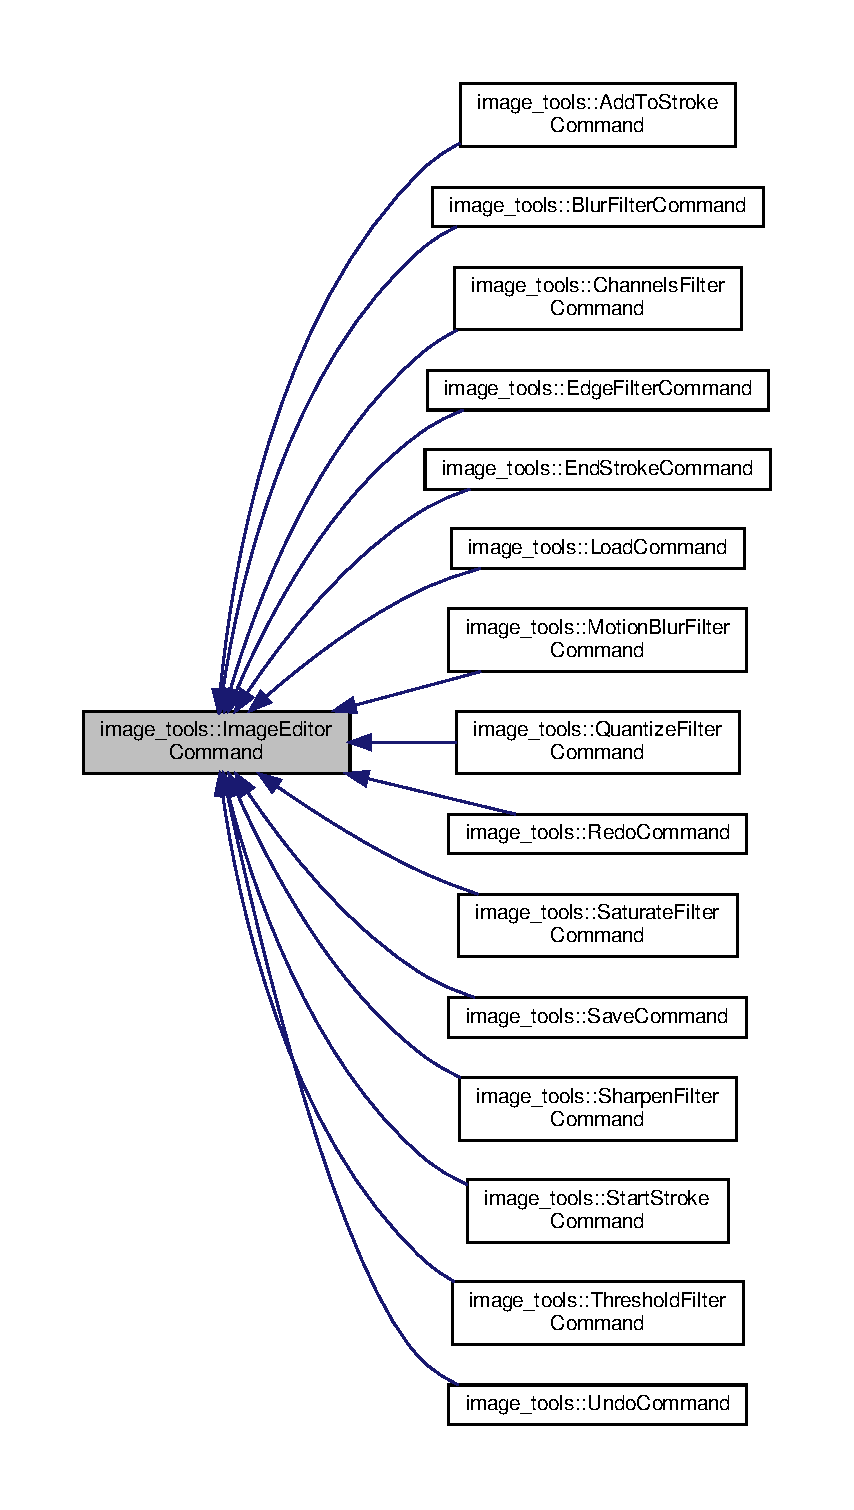
\includegraphics[height=550pt]{classimage__tools_1_1ImageEditorCommand__inherit__graph}
\end{center}
\end{figure}


Collaboration diagram for image\+\_\+tools\+:\+:Image\+Editor\+Command\+:
\nopagebreak
\begin{figure}[H]
\begin{center}
\leavevmode
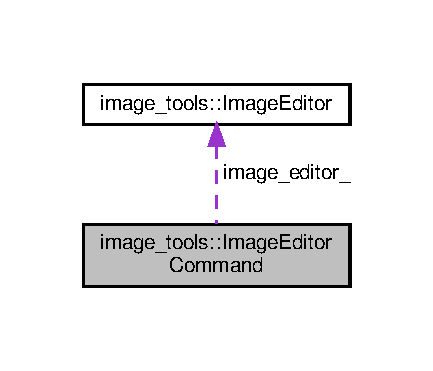
\includegraphics[width=208pt]{classimage__tools_1_1ImageEditorCommand__coll__graph}
\end{center}
\end{figure}
\subsection*{Public Member Functions}
\begin{DoxyCompactItemize}
\item 
\mbox{\Hypertarget{classimage__tools_1_1ImageEditorCommand_ac2843ecf9bcbae0dcb88b0eb081612e6}\label{classimage__tools_1_1ImageEditorCommand_ac2843ecf9bcbae0dcb88b0eb081612e6}} 
{\bfseries Image\+Editor\+Command} (\hyperlink{classimage__tools_1_1ImageEditor}{Image\+Editor} $\ast$image\+\_\+editor)
\item 
\mbox{\Hypertarget{classimage__tools_1_1ImageEditorCommand_aed20aa0ff8ae87c92c35ec2d445ffe96}\label{classimage__tools_1_1ImageEditorCommand_aed20aa0ff8ae87c92c35ec2d445ffe96}} 
virtual void {\bfseries Execute} ()=0
\end{DoxyCompactItemize}
\subsection*{Protected Attributes}
\begin{DoxyCompactItemize}
\item 
\mbox{\Hypertarget{classimage__tools_1_1ImageEditorCommand_a2b973bf000632c7767a29ca979dd3ef8}\label{classimage__tools_1_1ImageEditorCommand_a2b973bf000632c7767a29ca979dd3ef8}} 
\hyperlink{classimage__tools_1_1ImageEditor}{Image\+Editor} $\ast$ {\bfseries image\+\_\+editor\+\_\+}
\end{DoxyCompactItemize}


\subsection{Detailed Description}
Base class for all image editor commands. Each command knows how to execute itself, including sending and required parameters to the image editor. This structure follows the Command Design Pattern. The command pattern is also often used to implement undo. However, we don\textquotesingle{}t do that here because all of the commands get \char`\"{}undone\char`\"{} in exactly the same way -- we simply restore the pixel buffer that was in place before the command was executed. So, it\textquotesingle{}s quite clean to implement the undo feature directly within the \hyperlink{classimage__tools_1_1ImageEditor}{Image\+Editor} class, which simply maintains a list of previous pixel buffers. The main reason for implementing these command wrappers around the image editor functionality is to be able to easily create a list of commands to run later while parsing command line arguments. If instead we just processed each command as it appears on the command line (e.\+g., blur then threshold then ...) the process can potentially run for quite a long time before discovering that there is an error in the syntax at the end of the command line. So, it is nice to be able to parse the whole command line first building up a list of commands to send to the image editor and then, if the whole command line looks good, run the whole list of commands. 

The documentation for this class was generated from the following files\+:\begin{DoxyCompactItemize}
\item 
src/mia/image\+\_\+editor\+\_\+commands.\+h\item 
src/mia/image\+\_\+editor\+\_\+commands.\+cc\end{DoxyCompactItemize}

\hypertarget{classimage__tools_1_1ImageToolsMath}{}\section{image\+\_\+tools\+:\+:Image\+Tools\+Math Class Reference}
\label{classimage__tools_1_1ImageToolsMath}\index{image\+\_\+tools\+::\+Image\+Tools\+Math@{image\+\_\+tools\+::\+Image\+Tools\+Math}}


{\ttfamily \#include $<$image\+\_\+tools\+\_\+math.\+h$>$}

\subsection*{Static Public Member Functions}
\begin{DoxyCompactItemize}
\item 
\mbox{\Hypertarget{classimage__tools_1_1ImageToolsMath_a3551d9e654b48b3c0720176f0b925f1e}\label{classimage__tools_1_1ImageToolsMath_a3551d9e654b48b3c0720176f0b925f1e}} 
{\footnotesize template$<$typename T $>$ }\\static T \hyperlink{classimage__tools_1_1ImageToolsMath_a3551d9e654b48b3c0720176f0b925f1e}{Lerp} (T a, T b, float r)
\begin{DoxyCompactList}\small\item\em Linear interpolation between 2 two elements by a factor r. \end{DoxyCompactList}\item 
\mbox{\Hypertarget{classimage__tools_1_1ImageToolsMath_a3b03e68d10aa6f63037fd57f1cb77e96}\label{classimage__tools_1_1ImageToolsMath_a3b03e68d10aa6f63037fd57f1cb77e96}} 
{\footnotesize template$<$typename T $>$ }\\static T \hyperlink{classimage__tools_1_1ImageToolsMath_a3b03e68d10aa6f63037fd57f1cb77e96}{Clamp} (T x, T low, T high)
\begin{DoxyCompactList}\small\item\em Clamp the value of a type between \mbox{[}high,low\mbox{]} (inclusive). \end{DoxyCompactList}\item 
\mbox{\Hypertarget{classimage__tools_1_1ImageToolsMath_aa0518f431a7fd7feb691f3d36151082f}\label{classimage__tools_1_1ImageToolsMath_aa0518f431a7fd7feb691f3d36151082f}} 
static float \hyperlink{classimage__tools_1_1ImageToolsMath_aa0518f431a7fd7feb691f3d36151082f}{Gaussian} (float x, float sigma)
\begin{DoxyCompactList}\small\item\em Get the std deviation of a value in a gaussian distribution. \end{DoxyCompactList}\end{DoxyCompactItemize}


\subsection{Detailed Description}
A static class that holds several small math-\/related functions that are useful for manipulating images. 

The documentation for this class was generated from the following file\+:\begin{DoxyCompactItemize}
\item 
src/imagetools/image\+\_\+tools\+\_\+math.\+h\end{DoxyCompactItemize}

\hypertarget{classimage__tools_1_1LoadCommand}{}\section{image\+\_\+tools\+:\+:Load\+Command Class Reference}
\label{classimage__tools_1_1LoadCommand}\index{image\+\_\+tools\+::\+Load\+Command@{image\+\_\+tools\+::\+Load\+Command}}


{\ttfamily \#include $<$image\+\_\+editor\+\_\+commands.\+h$>$}



Inheritance diagram for image\+\_\+tools\+:\+:Load\+Command\+:
\nopagebreak
\begin{figure}[H]
\begin{center}
\leavevmode
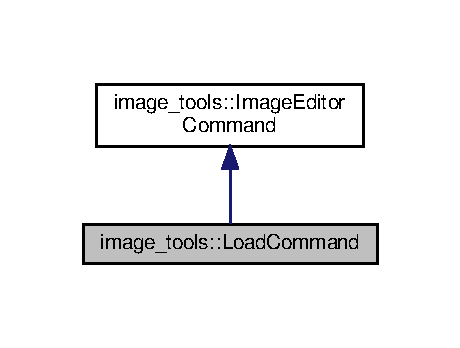
\includegraphics[width=221pt]{classimage__tools_1_1LoadCommand__inherit__graph}
\end{center}
\end{figure}


Collaboration diagram for image\+\_\+tools\+:\+:Load\+Command\+:
\nopagebreak
\begin{figure}[H]
\begin{center}
\leavevmode
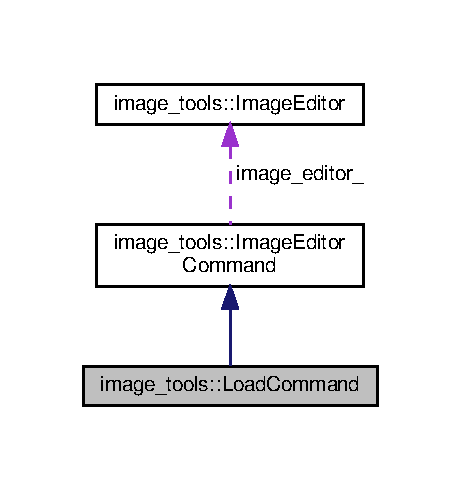
\includegraphics[width=221pt]{classimage__tools_1_1LoadCommand__coll__graph}
\end{center}
\end{figure}
\subsection*{Public Member Functions}
\begin{DoxyCompactItemize}
\item 
\mbox{\Hypertarget{classimage__tools_1_1LoadCommand_a713b9437101305d112320436afc351dd}\label{classimage__tools_1_1LoadCommand_a713b9437101305d112320436afc351dd}} 
{\bfseries Load\+Command} (\hyperlink{classimage__tools_1_1ImageEditor}{Image\+Editor} $\ast$image\+\_\+editor, const std\+::string \&filename)
\item 
\mbox{\Hypertarget{classimage__tools_1_1LoadCommand_ad0fcc08b3946955ece01a14e961815a7}\label{classimage__tools_1_1LoadCommand_ad0fcc08b3946955ece01a14e961815a7}} 
void {\bfseries Execute} () override
\end{DoxyCompactItemize}
\subsection*{Additional Inherited Members}


\subsection{Detailed Description}
Specific command for loading a file. 

The documentation for this class was generated from the following files\+:\begin{DoxyCompactItemize}
\item 
src/mia/image\+\_\+editor\+\_\+commands.\+h\item 
src/mia/image\+\_\+editor\+\_\+commands.\+cc\end{DoxyCompactItemize}

\hypertarget{classimage__tools_1_1MaskFactory}{}\section{image\+\_\+tools\+:\+:Mask\+Factory Class Reference}
\label{classimage__tools_1_1MaskFactory}\index{image\+\_\+tools\+::\+Mask\+Factory@{image\+\_\+tools\+::\+Mask\+Factory}}


{\ttfamily \#include $<$mask\+\_\+factory.\+h$>$}

\subsection*{Static Public Member Functions}
\begin{DoxyCompactItemize}
\item 
\mbox{\Hypertarget{classimage__tools_1_1MaskFactory_a4295a2802f73937d77a90d4f1fb60e24}\label{classimage__tools_1_1MaskFactory_a4295a2802f73937d77a90d4f1fb60e24}} 
static \hyperlink{classimage__tools_1_1FloatMatrix}{Float\+Matrix} $\ast$ {\bfseries Create\+Constant\+Mask} (float radius)
\item 
\mbox{\Hypertarget{classimage__tools_1_1MaskFactory_a039d26821cc56aca61a16b9e55266d9a}\label{classimage__tools_1_1MaskFactory_a039d26821cc56aca61a16b9e55266d9a}} 
static \hyperlink{classimage__tools_1_1FloatMatrix}{Float\+Matrix} $\ast$ {\bfseries Create\+Oval\+Mask} (float radius, float angle\+\_\+in\+\_\+deg, float ratio)
\item 
\mbox{\Hypertarget{classimage__tools_1_1MaskFactory_af7b0ecc4f1a758de1652fe4779556313}\label{classimage__tools_1_1MaskFactory_af7b0ecc4f1a758de1652fe4779556313}} 
static \hyperlink{classimage__tools_1_1FloatMatrix}{Float\+Matrix} $\ast$ {\bfseries Create\+Linear\+Falloff\+Mask} (float radius)
\item 
\mbox{\Hypertarget{classimage__tools_1_1MaskFactory_ac2d7a5a550904745bdb9ec82e5f6e9db}\label{classimage__tools_1_1MaskFactory_ac2d7a5a550904745bdb9ec82e5f6e9db}} 
static \hyperlink{classimage__tools_1_1FloatMatrix}{Float\+Matrix} $\ast$ {\bfseries Create\+Bullseye\+Mask} (float radius, float linewidth)
\end{DoxyCompactItemize}


\subsection{Detailed Description}
This factory is used to create masks used by image editing tools. Some of the masks are used by more than one tool. 

The documentation for this class was generated from the following files\+:\begin{DoxyCompactItemize}
\item 
src/imagetools/mask\+\_\+factory.\+h\item 
src/imagetools/mask\+\_\+factory.\+cc\end{DoxyCompactItemize}

\hypertarget{classimage__tools_1_1MiaApp}{}\section{image\+\_\+tools\+:\+:Mia\+App Class Reference}
\label{classimage__tools_1_1MiaApp}\index{image\+\_\+tools\+::\+Mia\+App@{image\+\_\+tools\+::\+Mia\+App}}


The Mia G\+UI. This class creates a graphics window to display the current \hyperlink{classimage__tools_1_1PixelBuffer}{Pixel\+Buffer} and a graphical user interface to interact with it using Tools and Filters.  




{\ttfamily \#include $<$mia\+\_\+app.\+h$>$}



Inheritance diagram for image\+\_\+tools\+:\+:Mia\+App\+:
\nopagebreak
\begin{figure}[H]
\begin{center}
\leavevmode
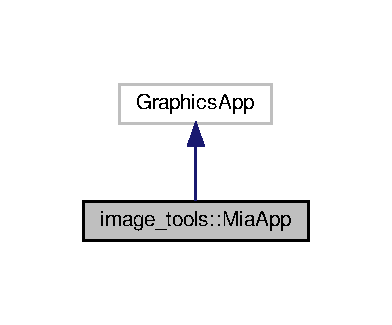
\includegraphics[width=188pt]{classimage__tools_1_1MiaApp__inherit__graph}
\end{center}
\end{figure}


Collaboration diagram for image\+\_\+tools\+:\+:Mia\+App\+:
\nopagebreak
\begin{figure}[H]
\begin{center}
\leavevmode
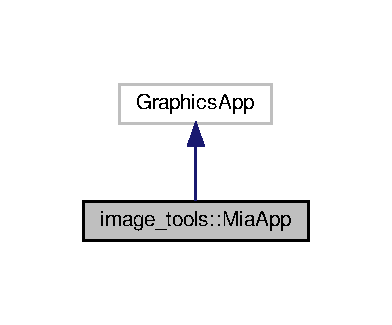
\includegraphics[width=188pt]{classimage__tools_1_1MiaApp__coll__graph}
\end{center}
\end{figure}
\subsection*{Public Member Functions}
\begin{DoxyCompactItemize}
\item 
\mbox{\Hypertarget{classimage__tools_1_1MiaApp_a615e8559a662c54a9f2487a7d6a55b57}\label{classimage__tools_1_1MiaApp_a615e8559a662c54a9f2487a7d6a55b57}} 
{\bfseries Mia\+App} (int width, int height, const \hyperlink{classimage__tools_1_1ColorData}{Color\+Data} \&background\+\_\+color)
\item 
void \hyperlink{classimage__tools_1_1MiaApp_a2b65628198da98dec676c57af8ff881c}{On\+Mouse\+Move} (const mingfx\+::\+Point2 \&pos, const mingfx\+::\+Vector2 \&delta) override
\item 
void \hyperlink{classimage__tools_1_1MiaApp_add49ee649aa2cd4f5a48cbe7ce932011}{On\+Left\+Mouse\+Down} (const mingfx\+::\+Point2 \&pos) override
\item 
void \hyperlink{classimage__tools_1_1MiaApp_a0a2f072e2a386bffd3ea9925807d1381}{On\+Left\+Mouse\+Drag} (const mingfx\+::\+Point2 \&pos, const mingfx\+::\+Vector2 \&delta) override
\item 
void \hyperlink{classimage__tools_1_1MiaApp_af386887e8245037fed9d615890cee417}{On\+Left\+Mouse\+Up} (const mingfx\+::\+Point2 \&pos) override
\item 
void \hyperlink{classimage__tools_1_1MiaApp_a81597364eeca01df8e26cfb6bf037ffe}{On\+Window\+Resize} (int new\+\_\+width, int new\+\_\+height) override
\item 
void \hyperlink{classimage__tools_1_1MiaApp_a601e7b8b38ca77b8c6bf81b421fda18b}{Update\+Simulation} (double dt) override
\item 
void \hyperlink{classimage__tools_1_1MiaApp_a83654a0b4e70c1b6b16e1b10d9becaad}{Init\+Nano\+G\+UI} () override
\item 
void \hyperlink{classimage__tools_1_1MiaApp_ac59579850ed3ebdfcc1885f88238e887}{Init\+Open\+GL} () override
\item 
void \hyperlink{classimage__tools_1_1MiaApp_af7498f998abe700b139f8600eb9e882b}{Draw\+Using\+Nano\+VG} (N\+V\+Gcontext $\ast$ctx) override
\item 
void \hyperlink{classimage__tools_1_1MiaApp_a0633d685229af3678546abcf1515362f}{Draw\+Using\+Open\+GL} () override
\end{DoxyCompactItemize}


\subsection{Detailed Description}
The Mia G\+UI. This class creates a graphics window to display the current \hyperlink{classimage__tools_1_1PixelBuffer}{Pixel\+Buffer} and a graphical user interface to interact with it using Tools and Filters. 

\subsection{Member Function Documentation}
\mbox{\Hypertarget{classimage__tools_1_1MiaApp_af7498f998abe700b139f8600eb9e882b}\label{classimage__tools_1_1MiaApp_af7498f998abe700b139f8600eb9e882b}} 
\index{image\+\_\+tools\+::\+Mia\+App@{image\+\_\+tools\+::\+Mia\+App}!Draw\+Using\+Nano\+VG@{Draw\+Using\+Nano\+VG}}
\index{Draw\+Using\+Nano\+VG@{Draw\+Using\+Nano\+VG}!image\+\_\+tools\+::\+Mia\+App@{image\+\_\+tools\+::\+Mia\+App}}
\subsubsection{\texorpdfstring{Draw\+Using\+Nano\+V\+G()}{DrawUsingNanoVG()}}
{\footnotesize\ttfamily void image\+\_\+tools\+::\+Mia\+App\+::\+Draw\+Using\+Nano\+VG (\begin{DoxyParamCaption}\item[{N\+V\+Gcontext $\ast$}]{ctx }\end{DoxyParamCaption})\hspace{0.3cm}{\ttfamily [override]}}

Used to draw the cursor for the tool once each frame. \mbox{\Hypertarget{classimage__tools_1_1MiaApp_a0633d685229af3678546abcf1515362f}\label{classimage__tools_1_1MiaApp_a0633d685229af3678546abcf1515362f}} 
\index{image\+\_\+tools\+::\+Mia\+App@{image\+\_\+tools\+::\+Mia\+App}!Draw\+Using\+Open\+GL@{Draw\+Using\+Open\+GL}}
\index{Draw\+Using\+Open\+GL@{Draw\+Using\+Open\+GL}!image\+\_\+tools\+::\+Mia\+App@{image\+\_\+tools\+::\+Mia\+App}}
\subsubsection{\texorpdfstring{Draw\+Using\+Open\+G\+L()}{DrawUsingOpenGL()}}
{\footnotesize\ttfamily void image\+\_\+tools\+::\+Mia\+App\+::\+Draw\+Using\+Open\+GL (\begin{DoxyParamCaption}{ }\end{DoxyParamCaption})\hspace{0.3cm}{\ttfamily [override]}}

Used to draw the \hyperlink{classimage__tools_1_1PixelBuffer}{Pixel\+Buffer} to the screen once each frame. \mbox{\Hypertarget{classimage__tools_1_1MiaApp_a83654a0b4e70c1b6b16e1b10d9becaad}\label{classimage__tools_1_1MiaApp_a83654a0b4e70c1b6b16e1b10d9becaad}} 
\index{image\+\_\+tools\+::\+Mia\+App@{image\+\_\+tools\+::\+Mia\+App}!Init\+Nano\+G\+UI@{Init\+Nano\+G\+UI}}
\index{Init\+Nano\+G\+UI@{Init\+Nano\+G\+UI}!image\+\_\+tools\+::\+Mia\+App@{image\+\_\+tools\+::\+Mia\+App}}
\subsubsection{\texorpdfstring{Init\+Nano\+G\+U\+I()}{InitNanoGUI()}}
{\footnotesize\ttfamily void image\+\_\+tools\+::\+Mia\+App\+::\+Init\+Nano\+G\+UI (\begin{DoxyParamCaption}{ }\end{DoxyParamCaption})\hspace{0.3cm}{\ttfamily [override]}}

Used to setup the 2D G\+UI. \mbox{\Hypertarget{classimage__tools_1_1MiaApp_ac59579850ed3ebdfcc1885f88238e887}\label{classimage__tools_1_1MiaApp_ac59579850ed3ebdfcc1885f88238e887}} 
\index{image\+\_\+tools\+::\+Mia\+App@{image\+\_\+tools\+::\+Mia\+App}!Init\+Open\+GL@{Init\+Open\+GL}}
\index{Init\+Open\+GL@{Init\+Open\+GL}!image\+\_\+tools\+::\+Mia\+App@{image\+\_\+tools\+::\+Mia\+App}}
\subsubsection{\texorpdfstring{Init\+Open\+G\+L()}{InitOpenGL()}}
{\footnotesize\ttfamily void image\+\_\+tools\+::\+Mia\+App\+::\+Init\+Open\+GL (\begin{DoxyParamCaption}{ }\end{DoxyParamCaption})\hspace{0.3cm}{\ttfamily [override]}}

Used to initialize Open\+GL graphics, including the texture used to draw the pixel buffer to the screen. \mbox{\Hypertarget{classimage__tools_1_1MiaApp_add49ee649aa2cd4f5a48cbe7ce932011}\label{classimage__tools_1_1MiaApp_add49ee649aa2cd4f5a48cbe7ce932011}} 
\index{image\+\_\+tools\+::\+Mia\+App@{image\+\_\+tools\+::\+Mia\+App}!On\+Left\+Mouse\+Down@{On\+Left\+Mouse\+Down}}
\index{On\+Left\+Mouse\+Down@{On\+Left\+Mouse\+Down}!image\+\_\+tools\+::\+Mia\+App@{image\+\_\+tools\+::\+Mia\+App}}
\subsubsection{\texorpdfstring{On\+Left\+Mouse\+Down()}{OnLeftMouseDown()}}
{\footnotesize\ttfamily void image\+\_\+tools\+::\+Mia\+App\+::\+On\+Left\+Mouse\+Down (\begin{DoxyParamCaption}\item[{const mingfx\+::\+Point2 \&}]{pos }\end{DoxyParamCaption})\hspace{0.3cm}{\ttfamily [override]}}

Called when the user pushes the mouse left button. \mbox{\Hypertarget{classimage__tools_1_1MiaApp_a0a2f072e2a386bffd3ea9925807d1381}\label{classimage__tools_1_1MiaApp_a0a2f072e2a386bffd3ea9925807d1381}} 
\index{image\+\_\+tools\+::\+Mia\+App@{image\+\_\+tools\+::\+Mia\+App}!On\+Left\+Mouse\+Drag@{On\+Left\+Mouse\+Drag}}
\index{On\+Left\+Mouse\+Drag@{On\+Left\+Mouse\+Drag}!image\+\_\+tools\+::\+Mia\+App@{image\+\_\+tools\+::\+Mia\+App}}
\subsubsection{\texorpdfstring{On\+Left\+Mouse\+Drag()}{OnLeftMouseDrag()}}
{\footnotesize\ttfamily void image\+\_\+tools\+::\+Mia\+App\+::\+On\+Left\+Mouse\+Drag (\begin{DoxyParamCaption}\item[{const mingfx\+::\+Point2 \&}]{pos,  }\item[{const mingfx\+::\+Vector2 \&}]{delta }\end{DoxyParamCaption})\hspace{0.3cm}{\ttfamily [override]}}

Called when the user moves the mouse with the left button depressed. \mbox{\Hypertarget{classimage__tools_1_1MiaApp_af386887e8245037fed9d615890cee417}\label{classimage__tools_1_1MiaApp_af386887e8245037fed9d615890cee417}} 
\index{image\+\_\+tools\+::\+Mia\+App@{image\+\_\+tools\+::\+Mia\+App}!On\+Left\+Mouse\+Up@{On\+Left\+Mouse\+Up}}
\index{On\+Left\+Mouse\+Up@{On\+Left\+Mouse\+Up}!image\+\_\+tools\+::\+Mia\+App@{image\+\_\+tools\+::\+Mia\+App}}
\subsubsection{\texorpdfstring{On\+Left\+Mouse\+Up()}{OnLeftMouseUp()}}
{\footnotesize\ttfamily void image\+\_\+tools\+::\+Mia\+App\+::\+On\+Left\+Mouse\+Up (\begin{DoxyParamCaption}\item[{const mingfx\+::\+Point2 \&}]{pos }\end{DoxyParamCaption})\hspace{0.3cm}{\ttfamily [override]}}

Called when the user releases the left mouse button. \mbox{\Hypertarget{classimage__tools_1_1MiaApp_a2b65628198da98dec676c57af8ff881c}\label{classimage__tools_1_1MiaApp_a2b65628198da98dec676c57af8ff881c}} 
\index{image\+\_\+tools\+::\+Mia\+App@{image\+\_\+tools\+::\+Mia\+App}!On\+Mouse\+Move@{On\+Mouse\+Move}}
\index{On\+Mouse\+Move@{On\+Mouse\+Move}!image\+\_\+tools\+::\+Mia\+App@{image\+\_\+tools\+::\+Mia\+App}}
\subsubsection{\texorpdfstring{On\+Mouse\+Move()}{OnMouseMove()}}
{\footnotesize\ttfamily void image\+\_\+tools\+::\+Mia\+App\+::\+On\+Mouse\+Move (\begin{DoxyParamCaption}\item[{const mingfx\+::\+Point2 \&}]{pos,  }\item[{const mingfx\+::\+Vector2 \&}]{delta }\end{DoxyParamCaption})\hspace{0.3cm}{\ttfamily [override]}}

Called when the mouse moves but no mouse buttons are currently pressed. \mbox{\Hypertarget{classimage__tools_1_1MiaApp_a81597364eeca01df8e26cfb6bf037ffe}\label{classimage__tools_1_1MiaApp_a81597364eeca01df8e26cfb6bf037ffe}} 
\index{image\+\_\+tools\+::\+Mia\+App@{image\+\_\+tools\+::\+Mia\+App}!On\+Window\+Resize@{On\+Window\+Resize}}
\index{On\+Window\+Resize@{On\+Window\+Resize}!image\+\_\+tools\+::\+Mia\+App@{image\+\_\+tools\+::\+Mia\+App}}
\subsubsection{\texorpdfstring{On\+Window\+Resize()}{OnWindowResize()}}
{\footnotesize\ttfamily void image\+\_\+tools\+::\+Mia\+App\+::\+On\+Window\+Resize (\begin{DoxyParamCaption}\item[{int}]{new\+\_\+width,  }\item[{int}]{new\+\_\+height }\end{DoxyParamCaption})\hspace{0.3cm}{\ttfamily [override]}}

This function is called when the user drags the corner of the window to resize it. We need to detect that operation because it requires us to resize the underlying pixel buffer. \mbox{\Hypertarget{classimage__tools_1_1MiaApp_a601e7b8b38ca77b8c6bf81b421fda18b}\label{classimage__tools_1_1MiaApp_a601e7b8b38ca77b8c6bf81b421fda18b}} 
\index{image\+\_\+tools\+::\+Mia\+App@{image\+\_\+tools\+::\+Mia\+App}!Update\+Simulation@{Update\+Simulation}}
\index{Update\+Simulation@{Update\+Simulation}!image\+\_\+tools\+::\+Mia\+App@{image\+\_\+tools\+::\+Mia\+App}}
\subsubsection{\texorpdfstring{Update\+Simulation()}{UpdateSimulation()}}
{\footnotesize\ttfamily void image\+\_\+tools\+::\+Mia\+App\+::\+Update\+Simulation (\begin{DoxyParamCaption}\item[{double}]{dt }\end{DoxyParamCaption})\hspace{0.3cm}{\ttfamily [override]}}

This function gets called once per frame. If the user is in the middle of using a tool that applies more \char`\"{}paint\char`\"{} over time, like a spray can, then this function is used to repeatedly apply the tool to the pixel buffer. 

The documentation for this class was generated from the following files\+:\begin{DoxyCompactItemize}
\item 
src/mia/mia\+\_\+app.\+h\item 
src/mia/mia\+\_\+app.\+cc\end{DoxyCompactItemize}

\hypertarget{classimage__tools_1_1MotionBlurFilterCommand}{}\section{image\+\_\+tools\+:\+:Motion\+Blur\+Filter\+Command Class Reference}
\label{classimage__tools_1_1MotionBlurFilterCommand}\index{image\+\_\+tools\+::\+Motion\+Blur\+Filter\+Command@{image\+\_\+tools\+::\+Motion\+Blur\+Filter\+Command}}


{\ttfamily \#include $<$image\+\_\+editor\+\_\+commands.\+h$>$}



Inheritance diagram for image\+\_\+tools\+:\+:Motion\+Blur\+Filter\+Command\+:
\nopagebreak
\begin{figure}[H]
\begin{center}
\leavevmode
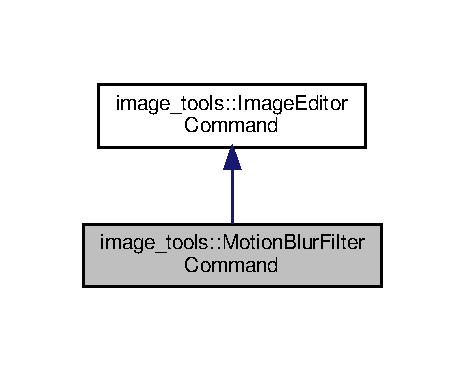
\includegraphics[width=223pt]{classimage__tools_1_1MotionBlurFilterCommand__inherit__graph}
\end{center}
\end{figure}


Collaboration diagram for image\+\_\+tools\+:\+:Motion\+Blur\+Filter\+Command\+:
\nopagebreak
\begin{figure}[H]
\begin{center}
\leavevmode
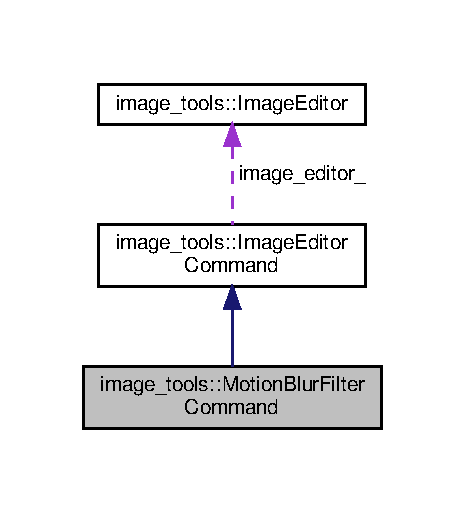
\includegraphics[width=223pt]{classimage__tools_1_1MotionBlurFilterCommand__coll__graph}
\end{center}
\end{figure}
\subsection*{Public Member Functions}
\begin{DoxyCompactItemize}
\item 
\mbox{\Hypertarget{classimage__tools_1_1MotionBlurFilterCommand_a2a7024e58bd095b8b7f87f6987c7e11b}\label{classimage__tools_1_1MotionBlurFilterCommand_a2a7024e58bd095b8b7f87f6987c7e11b}} 
{\bfseries Motion\+Blur\+Filter\+Command} (\hyperlink{classimage__tools_1_1ImageEditor}{Image\+Editor} $\ast$image\+\_\+editor, float radius, \hyperlink{classimage__tools_1_1ImageEditor_a20bacf2756f1b97eed82d2fee9628ac2}{Image\+Editor\+::\+M\+Blur\+Dir} dir)
\item 
\mbox{\Hypertarget{classimage__tools_1_1MotionBlurFilterCommand_a1c267e42f069322158770d97a4bd8c18}\label{classimage__tools_1_1MotionBlurFilterCommand_a1c267e42f069322158770d97a4bd8c18}} 
void {\bfseries Execute} () override
\end{DoxyCompactItemize}
\subsection*{Additional Inherited Members}


\subsection{Detailed Description}
Specific command for executing a motion blur filter. 

The documentation for this class was generated from the following files\+:\begin{DoxyCompactItemize}
\item 
src/mia/image\+\_\+editor\+\_\+commands.\+h\item 
src/mia/image\+\_\+editor\+\_\+commands.\+cc\end{DoxyCompactItemize}

\hypertarget{classimage__tools_1_1PixelBuffer}{}\section{image\+\_\+tools\+:\+:Pixel\+Buffer Class Reference}
\label{classimage__tools_1_1PixelBuffer}\index{image\+\_\+tools\+::\+Pixel\+Buffer@{image\+\_\+tools\+::\+Pixel\+Buffer}}


Stores an array of \hyperlink{classimage__tools_1_1ColorData}{Color\+Data}, such as an image that can be drawn to the screen.  




{\ttfamily \#include $<$pixel\+\_\+buffer.\+h$>$}

\subsection*{Public Member Functions}
\begin{DoxyCompactItemize}
\item 
\hyperlink{classimage__tools_1_1PixelBuffer_a4f5b5df93389946d70bc001acfebcedb}{Pixel\+Buffer} (int w, int h, \hyperlink{classimage__tools_1_1ColorData}{Color\+Data} \hyperlink{classimage__tools_1_1PixelBuffer_a3d6b71aeb5d7ec8a204aac67df7b83ac}{background\+\_\+color})
\item 
\hyperlink{classimage__tools_1_1PixelBuffer_a22e3446de759c42e6be6f290feca8461}{Pixel\+Buffer} (const std\+::string \&filename)
\item 
\hyperlink{classimage__tools_1_1PixelBuffer_a25b0c7d5686807d187ee799a5fbb1121}{Pixel\+Buffer} (const \hyperlink{classimage__tools_1_1PixelBuffer}{Pixel\+Buffer} \&rhs)
\item 
\hyperlink{classimage__tools_1_1PixelBuffer}{Pixel\+Buffer} \& \hyperlink{classimage__tools_1_1PixelBuffer_a95f63d0b72c4d0b371c556597cf77578}{operator=} (const \hyperlink{classimage__tools_1_1PixelBuffer}{Pixel\+Buffer} \&rhs)
\item 
\mbox{\Hypertarget{classimage__tools_1_1PixelBuffer_ab2bd64291a4275421bc72268da2143be}\label{classimage__tools_1_1PixelBuffer_ab2bd64291a4275421bc72268da2143be}} 
int {\bfseries height} () const
\item 
\mbox{\Hypertarget{classimage__tools_1_1PixelBuffer_a80cdd8ef54915b4549f8c6fc86f6dccc}\label{classimage__tools_1_1PixelBuffer_a80cdd8ef54915b4549f8c6fc86f6dccc}} 
int {\bfseries width} () const
\item 
const \hyperlink{classimage__tools_1_1ColorData}{Color\+Data} \& \hyperlink{classimage__tools_1_1PixelBuffer_a3d6b71aeb5d7ec8a204aac67df7b83ac}{background\+\_\+color} () const
\begin{DoxyCompactList}\small\item\em Get the background color that was used to initialize the \hyperlink{classimage__tools_1_1PixelBuffer}{Pixel\+Buffer}. \end{DoxyCompactList}\item 
\mbox{\Hypertarget{classimage__tools_1_1PixelBuffer_a4321d9a8751015b998ce51c59f0a94b9}\label{classimage__tools_1_1PixelBuffer_a4321d9a8751015b998ce51c59f0a94b9}} 
\hyperlink{classimage__tools_1_1ColorData}{Color\+Data} \hyperlink{classimage__tools_1_1PixelBuffer_a4321d9a8751015b998ce51c59f0a94b9}{pixel} (int x, int y) const
\begin{DoxyCompactList}\small\item\em Get the color of a specific pixel. \end{DoxyCompactList}\item 
\mbox{\Hypertarget{classimage__tools_1_1PixelBuffer_ac3559133504c49f3af9a00544411c3b8}\label{classimage__tools_1_1PixelBuffer_ac3559133504c49f3af9a00544411c3b8}} 
void \hyperlink{classimage__tools_1_1PixelBuffer_ac3559133504c49f3af9a00544411c3b8}{set\+\_\+pixel} (int x, int y, const \hyperlink{classimage__tools_1_1ColorData}{Color\+Data} \&color)
\begin{DoxyCompactList}\small\item\em Set the value for a specific pixel. \end{DoxyCompactList}\item 
float const  $\ast$ \hyperlink{classimage__tools_1_1PixelBuffer_a8f7b9f293b7ac93f8c33f75f50ce5a7b}{data} () const
\item 
void \hyperlink{classimage__tools_1_1PixelBuffer_a001dbd44de2d3f19b04180cdbc897b97}{Resize} (int new\+\_\+width, int new\+\_\+height)
\item 
void \hyperlink{classimage__tools_1_1PixelBuffer_ae3f65414f52d3df79c89c88d2a4db288}{Save\+To\+File} (const std\+::string \&filename)
\item 
void \hyperlink{classimage__tools_1_1PixelBuffer_aaa5f861df2ec901617aadeb5016bdf1e}{Load\+From\+File} (const std\+::string \&filename)
\end{DoxyCompactItemize}
\subsection*{Friends}
\begin{DoxyCompactItemize}
\item 
bool \hyperlink{classimage__tools_1_1PixelBuffer_a68aef4100a6c7062d102b566dc382543}{operator==} (const \hyperlink{classimage__tools_1_1PixelBuffer}{Pixel\+Buffer} \&a, const \hyperlink{classimage__tools_1_1PixelBuffer}{Pixel\+Buffer} \&b)
\item 
bool \hyperlink{classimage__tools_1_1PixelBuffer_a9751369b6acaba6bc42143cc2b7314ea}{operator!=} (const \hyperlink{classimage__tools_1_1PixelBuffer}{Pixel\+Buffer} \&a, const \hyperlink{classimage__tools_1_1PixelBuffer}{Pixel\+Buffer} \&b)
\end{DoxyCompactItemize}


\subsection{Detailed Description}
Stores an array of \hyperlink{classimage__tools_1_1ColorData}{Color\+Data}, such as an image that can be drawn to the screen. 

The data are stored internally in a 1D array, laid out in row-\/major order with 4 floats (R\+G\+BA) for each pixel in the image. The raw data can be accessed directly with \hyperlink{classimage__tools_1_1PixelBuffer_a8f7b9f293b7ac93f8c33f75f50ce5a7b}{data()} and individual pixels can be accessed with get\+\_\+pixel(x,y). 

\subsection{Constructor \& Destructor Documentation}
\mbox{\Hypertarget{classimage__tools_1_1PixelBuffer_a4f5b5df93389946d70bc001acfebcedb}\label{classimage__tools_1_1PixelBuffer_a4f5b5df93389946d70bc001acfebcedb}} 
\index{image\+\_\+tools\+::\+Pixel\+Buffer@{image\+\_\+tools\+::\+Pixel\+Buffer}!Pixel\+Buffer@{Pixel\+Buffer}}
\index{Pixel\+Buffer@{Pixel\+Buffer}!image\+\_\+tools\+::\+Pixel\+Buffer@{image\+\_\+tools\+::\+Pixel\+Buffer}}
\subsubsection{\texorpdfstring{Pixel\+Buffer()}{PixelBuffer()}\hspace{0.1cm}{\footnotesize\ttfamily [1/3]}}
{\footnotesize\ttfamily image\+\_\+tools\+::\+Pixel\+Buffer\+::\+Pixel\+Buffer (\begin{DoxyParamCaption}\item[{int}]{w,  }\item[{int}]{h,  }\item[{\hyperlink{classimage__tools_1_1ColorData}{Color\+Data}}]{background\+\_\+color }\end{DoxyParamCaption})}

Fills the new pixel buffer with the background color. \mbox{\Hypertarget{classimage__tools_1_1PixelBuffer_a22e3446de759c42e6be6f290feca8461}\label{classimage__tools_1_1PixelBuffer_a22e3446de759c42e6be6f290feca8461}} 
\index{image\+\_\+tools\+::\+Pixel\+Buffer@{image\+\_\+tools\+::\+Pixel\+Buffer}!Pixel\+Buffer@{Pixel\+Buffer}}
\index{Pixel\+Buffer@{Pixel\+Buffer}!image\+\_\+tools\+::\+Pixel\+Buffer@{image\+\_\+tools\+::\+Pixel\+Buffer}}
\subsubsection{\texorpdfstring{Pixel\+Buffer()}{PixelBuffer()}\hspace{0.1cm}{\footnotesize\ttfamily [2/3]}}
{\footnotesize\ttfamily image\+\_\+tools\+::\+Pixel\+Buffer\+::\+Pixel\+Buffer (\begin{DoxyParamCaption}\item[{const std\+::string \&}]{filename }\end{DoxyParamCaption})\hspace{0.3cm}{\ttfamily [explicit]}}

Loads a P\+NG image and stores it in the buffer. Sets the background color to white. \mbox{\Hypertarget{classimage__tools_1_1PixelBuffer_a25b0c7d5686807d187ee799a5fbb1121}\label{classimage__tools_1_1PixelBuffer_a25b0c7d5686807d187ee799a5fbb1121}} 
\index{image\+\_\+tools\+::\+Pixel\+Buffer@{image\+\_\+tools\+::\+Pixel\+Buffer}!Pixel\+Buffer@{Pixel\+Buffer}}
\index{Pixel\+Buffer@{Pixel\+Buffer}!image\+\_\+tools\+::\+Pixel\+Buffer@{image\+\_\+tools\+::\+Pixel\+Buffer}}
\subsubsection{\texorpdfstring{Pixel\+Buffer()}{PixelBuffer()}\hspace{0.1cm}{\footnotesize\ttfamily [3/3]}}
{\footnotesize\ttfamily image\+\_\+tools\+::\+Pixel\+Buffer\+::\+Pixel\+Buffer (\begin{DoxyParamCaption}\item[{const \hyperlink{classimage__tools_1_1PixelBuffer}{Pixel\+Buffer} \&}]{rhs }\end{DoxyParamCaption})}

Copy constructor 

\subsection{Member Function Documentation}
\mbox{\Hypertarget{classimage__tools_1_1PixelBuffer_a3d6b71aeb5d7ec8a204aac67df7b83ac}\label{classimage__tools_1_1PixelBuffer_a3d6b71aeb5d7ec8a204aac67df7b83ac}} 
\index{image\+\_\+tools\+::\+Pixel\+Buffer@{image\+\_\+tools\+::\+Pixel\+Buffer}!background\+\_\+color@{background\+\_\+color}}
\index{background\+\_\+color@{background\+\_\+color}!image\+\_\+tools\+::\+Pixel\+Buffer@{image\+\_\+tools\+::\+Pixel\+Buffer}}
\subsubsection{\texorpdfstring{background\+\_\+color()}{background\_color()}}
{\footnotesize\ttfamily const \hyperlink{classimage__tools_1_1ColorData}{Color\+Data}\& image\+\_\+tools\+::\+Pixel\+Buffer\+::background\+\_\+color (\begin{DoxyParamCaption}{ }\end{DoxyParamCaption}) const\hspace{0.3cm}{\ttfamily [inline]}}



Get the background color that was used to initialize the \hyperlink{classimage__tools_1_1PixelBuffer}{Pixel\+Buffer}. 

\begin{DoxyReturn}{Returns}
The background color 
\end{DoxyReturn}
\mbox{\Hypertarget{classimage__tools_1_1PixelBuffer_a8f7b9f293b7ac93f8c33f75f50ce5a7b}\label{classimage__tools_1_1PixelBuffer_a8f7b9f293b7ac93f8c33f75f50ce5a7b}} 
\index{image\+\_\+tools\+::\+Pixel\+Buffer@{image\+\_\+tools\+::\+Pixel\+Buffer}!data@{data}}
\index{data@{data}!image\+\_\+tools\+::\+Pixel\+Buffer@{image\+\_\+tools\+::\+Pixel\+Buffer}}
\subsubsection{\texorpdfstring{data()}{data()}}
{\footnotesize\ttfamily float const$\ast$ image\+\_\+tools\+::\+Pixel\+Buffer\+::data (\begin{DoxyParamCaption}{ }\end{DoxyParamCaption}) const\hspace{0.3cm}{\ttfamily [inline]}}

Returns a pointer to the raw pixel data array stored in row-\/major order as R\+G\+BA floats. \mbox{\Hypertarget{classimage__tools_1_1PixelBuffer_aaa5f861df2ec901617aadeb5016bdf1e}\label{classimage__tools_1_1PixelBuffer_aaa5f861df2ec901617aadeb5016bdf1e}} 
\index{image\+\_\+tools\+::\+Pixel\+Buffer@{image\+\_\+tools\+::\+Pixel\+Buffer}!Load\+From\+File@{Load\+From\+File}}
\index{Load\+From\+File@{Load\+From\+File}!image\+\_\+tools\+::\+Pixel\+Buffer@{image\+\_\+tools\+::\+Pixel\+Buffer}}
\subsubsection{\texorpdfstring{Load\+From\+File()}{LoadFromFile()}}
{\footnotesize\ttfamily void image\+\_\+tools\+::\+Pixel\+Buffer\+::\+Load\+From\+File (\begin{DoxyParamCaption}\item[{const std\+::string \&}]{filename }\end{DoxyParamCaption})}

Loads from a P\+NG file. Will resize the buffer as needed. \mbox{\Hypertarget{classimage__tools_1_1PixelBuffer_a95f63d0b72c4d0b371c556597cf77578}\label{classimage__tools_1_1PixelBuffer_a95f63d0b72c4d0b371c556597cf77578}} 
\index{image\+\_\+tools\+::\+Pixel\+Buffer@{image\+\_\+tools\+::\+Pixel\+Buffer}!operator=@{operator=}}
\index{operator=@{operator=}!image\+\_\+tools\+::\+Pixel\+Buffer@{image\+\_\+tools\+::\+Pixel\+Buffer}}
\subsubsection{\texorpdfstring{operator=()}{operator=()}}
{\footnotesize\ttfamily \hyperlink{classimage__tools_1_1PixelBuffer}{Pixel\+Buffer} \& image\+\_\+tools\+::\+Pixel\+Buffer\+::operator= (\begin{DoxyParamCaption}\item[{const \hyperlink{classimage__tools_1_1PixelBuffer}{Pixel\+Buffer} \&}]{rhs }\end{DoxyParamCaption})}

Assignment operator \mbox{\Hypertarget{classimage__tools_1_1PixelBuffer_a001dbd44de2d3f19b04180cdbc897b97}\label{classimage__tools_1_1PixelBuffer_a001dbd44de2d3f19b04180cdbc897b97}} 
\index{image\+\_\+tools\+::\+Pixel\+Buffer@{image\+\_\+tools\+::\+Pixel\+Buffer}!Resize@{Resize}}
\index{Resize@{Resize}!image\+\_\+tools\+::\+Pixel\+Buffer@{image\+\_\+tools\+::\+Pixel\+Buffer}}
\subsubsection{\texorpdfstring{Resize()}{Resize()}}
{\footnotesize\ttfamily void image\+\_\+tools\+::\+Pixel\+Buffer\+::\+Resize (\begin{DoxyParamCaption}\item[{int}]{new\+\_\+width,  }\item[{int}]{new\+\_\+height }\end{DoxyParamCaption})}

Resizes the buffer, cropping the image and/or creating new pixels as needed. New pixels will use the background color. \mbox{\Hypertarget{classimage__tools_1_1PixelBuffer_ae3f65414f52d3df79c89c88d2a4db288}\label{classimage__tools_1_1PixelBuffer_ae3f65414f52d3df79c89c88d2a4db288}} 
\index{image\+\_\+tools\+::\+Pixel\+Buffer@{image\+\_\+tools\+::\+Pixel\+Buffer}!Save\+To\+File@{Save\+To\+File}}
\index{Save\+To\+File@{Save\+To\+File}!image\+\_\+tools\+::\+Pixel\+Buffer@{image\+\_\+tools\+::\+Pixel\+Buffer}}
\subsubsection{\texorpdfstring{Save\+To\+File()}{SaveToFile()}}
{\footnotesize\ttfamily void image\+\_\+tools\+::\+Pixel\+Buffer\+::\+Save\+To\+File (\begin{DoxyParamCaption}\item[{const std\+::string \&}]{filename }\end{DoxyParamCaption})}

Saves to a P\+NG file, the filename should include a .png extension. 

\subsection{Friends And Related Function Documentation}
\mbox{\Hypertarget{classimage__tools_1_1PixelBuffer_a9751369b6acaba6bc42143cc2b7314ea}\label{classimage__tools_1_1PixelBuffer_a9751369b6acaba6bc42143cc2b7314ea}} 
\index{image\+\_\+tools\+::\+Pixel\+Buffer@{image\+\_\+tools\+::\+Pixel\+Buffer}!operator"!=@{operator"!=}}
\index{operator"!=@{operator"!=}!image\+\_\+tools\+::\+Pixel\+Buffer@{image\+\_\+tools\+::\+Pixel\+Buffer}}
\subsubsection{\texorpdfstring{operator"!=}{operator!=}}
{\footnotesize\ttfamily bool operator!= (\begin{DoxyParamCaption}\item[{const \hyperlink{classimage__tools_1_1PixelBuffer}{Pixel\+Buffer} \&}]{a,  }\item[{const \hyperlink{classimage__tools_1_1PixelBuffer}{Pixel\+Buffer} \&}]{b }\end{DoxyParamCaption})\hspace{0.3cm}{\ttfamily [friend]}}

Check for \char`\"{}inequality\char`\"{}, taking floating point imprecision into account \mbox{\Hypertarget{classimage__tools_1_1PixelBuffer_a68aef4100a6c7062d102b566dc382543}\label{classimage__tools_1_1PixelBuffer_a68aef4100a6c7062d102b566dc382543}} 
\index{image\+\_\+tools\+::\+Pixel\+Buffer@{image\+\_\+tools\+::\+Pixel\+Buffer}!operator==@{operator==}}
\index{operator==@{operator==}!image\+\_\+tools\+::\+Pixel\+Buffer@{image\+\_\+tools\+::\+Pixel\+Buffer}}
\subsubsection{\texorpdfstring{operator==}{operator==}}
{\footnotesize\ttfamily bool operator== (\begin{DoxyParamCaption}\item[{const \hyperlink{classimage__tools_1_1PixelBuffer}{Pixel\+Buffer} \&}]{a,  }\item[{const \hyperlink{classimage__tools_1_1PixelBuffer}{Pixel\+Buffer} \&}]{b }\end{DoxyParamCaption})\hspace{0.3cm}{\ttfamily [friend]}}

Check for \char`\"{}equality\char`\"{}, taking floating point imprecision into account 

The documentation for this class was generated from the following files\+:\begin{DoxyCompactItemize}
\item 
src/imagetools/pixel\+\_\+buffer.\+h\item 
src/imagetools/pixel\+\_\+buffer.\+cc\end{DoxyCompactItemize}

\hypertarget{classimage__tools_1_1QuantizeFilterCommand}{}\section{image\+\_\+tools\+:\+:Quantize\+Filter\+Command Class Reference}
\label{classimage__tools_1_1QuantizeFilterCommand}\index{image\+\_\+tools\+::\+Quantize\+Filter\+Command@{image\+\_\+tools\+::\+Quantize\+Filter\+Command}}


{\ttfamily \#include $<$image\+\_\+editor\+\_\+commands.\+h$>$}



Inheritance diagram for image\+\_\+tools\+:\+:Quantize\+Filter\+Command\+:
\nopagebreak
\begin{figure}[H]
\begin{center}
\leavevmode
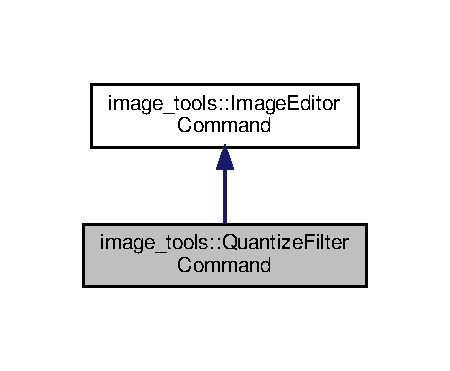
\includegraphics[width=216pt]{classimage__tools_1_1QuantizeFilterCommand__inherit__graph}
\end{center}
\end{figure}


Collaboration diagram for image\+\_\+tools\+:\+:Quantize\+Filter\+Command\+:
\nopagebreak
\begin{figure}[H]
\begin{center}
\leavevmode
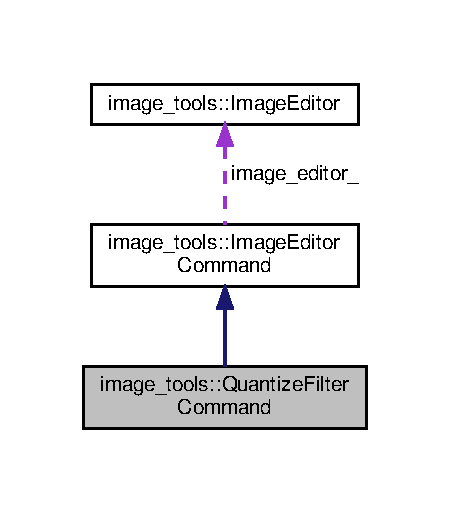
\includegraphics[width=216pt]{classimage__tools_1_1QuantizeFilterCommand__coll__graph}
\end{center}
\end{figure}
\subsection*{Public Member Functions}
\begin{DoxyCompactItemize}
\item 
\mbox{\Hypertarget{classimage__tools_1_1QuantizeFilterCommand_a47f3c67d8fffc4fe2be5999373bfb786}\label{classimage__tools_1_1QuantizeFilterCommand_a47f3c67d8fffc4fe2be5999373bfb786}} 
{\bfseries Quantize\+Filter\+Command} (\hyperlink{classimage__tools_1_1ImageEditor}{Image\+Editor} $\ast$image\+\_\+editor, int bins)
\item 
\mbox{\Hypertarget{classimage__tools_1_1QuantizeFilterCommand_a02b071572e9d690e636311ee633d6db4}\label{classimage__tools_1_1QuantizeFilterCommand_a02b071572e9d690e636311ee633d6db4}} 
void {\bfseries Execute} () override
\end{DoxyCompactItemize}
\subsection*{Additional Inherited Members}


\subsection{Detailed Description}
Specific command for executing a quantize filter. 

The documentation for this class was generated from the following files\+:\begin{DoxyCompactItemize}
\item 
src/mia/image\+\_\+editor\+\_\+commands.\+h\item 
src/mia/image\+\_\+editor\+\_\+commands.\+cc\end{DoxyCompactItemize}

\hypertarget{classimage__tools_1_1RedoCommand}{}\section{image\+\_\+tools\+:\+:Redo\+Command Class Reference}
\label{classimage__tools_1_1RedoCommand}\index{image\+\_\+tools\+::\+Redo\+Command@{image\+\_\+tools\+::\+Redo\+Command}}


{\ttfamily \#include $<$image\+\_\+editor\+\_\+commands.\+h$>$}



Inheritance diagram for image\+\_\+tools\+:\+:Redo\+Command\+:
\nopagebreak
\begin{figure}[H]
\begin{center}
\leavevmode
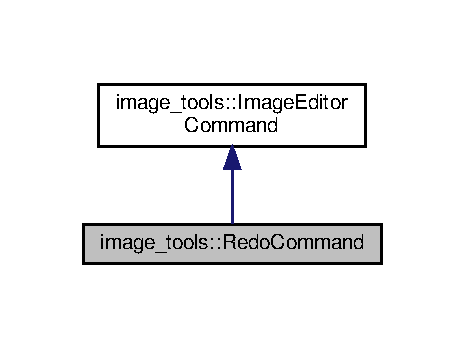
\includegraphics[width=223pt]{classimage__tools_1_1RedoCommand__inherit__graph}
\end{center}
\end{figure}


Collaboration diagram for image\+\_\+tools\+:\+:Redo\+Command\+:
\nopagebreak
\begin{figure}[H]
\begin{center}
\leavevmode
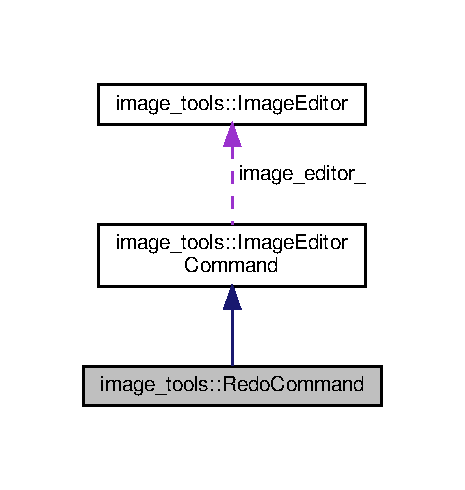
\includegraphics[width=223pt]{classimage__tools_1_1RedoCommand__coll__graph}
\end{center}
\end{figure}
\subsection*{Public Member Functions}
\begin{DoxyCompactItemize}
\item 
\mbox{\Hypertarget{classimage__tools_1_1RedoCommand_a7077e1a8dab12f4d941ec8cc1431fcbb}\label{classimage__tools_1_1RedoCommand_a7077e1a8dab12f4d941ec8cc1431fcbb}} 
{\bfseries Redo\+Command} (\hyperlink{classimage__tools_1_1ImageEditor}{Image\+Editor} $\ast$image\+\_\+editor)
\item 
\mbox{\Hypertarget{classimage__tools_1_1RedoCommand_abd1811d6cba4a95c949e963a6753137f}\label{classimage__tools_1_1RedoCommand_abd1811d6cba4a95c949e963a6753137f}} 
void {\bfseries Execute} () override
\end{DoxyCompactItemize}
\subsection*{Additional Inherited Members}


\subsection{Detailed Description}
Specific command for executing a redo. 

The documentation for this class was generated from the following files\+:\begin{DoxyCompactItemize}
\item 
src/mia/image\+\_\+editor\+\_\+commands.\+h\item 
src/mia/image\+\_\+editor\+\_\+commands.\+cc\end{DoxyCompactItemize}

\hypertarget{classimage__tools_1_1SaturateFilterCommand}{}\section{image\+\_\+tools\+:\+:Saturate\+Filter\+Command Class Reference}
\label{classimage__tools_1_1SaturateFilterCommand}\index{image\+\_\+tools\+::\+Saturate\+Filter\+Command@{image\+\_\+tools\+::\+Saturate\+Filter\+Command}}


{\ttfamily \#include $<$image\+\_\+editor\+\_\+commands.\+h$>$}



Inheritance diagram for image\+\_\+tools\+:\+:Saturate\+Filter\+Command\+:
\nopagebreak
\begin{figure}[H]
\begin{center}
\leavevmode
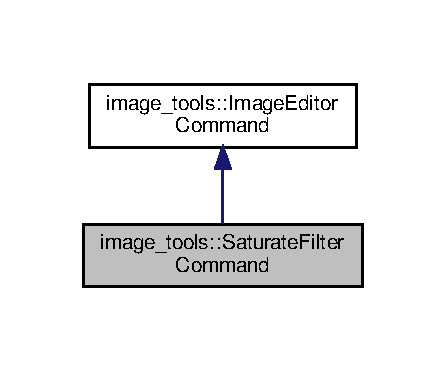
\includegraphics[width=214pt]{classimage__tools_1_1SaturateFilterCommand__inherit__graph}
\end{center}
\end{figure}


Collaboration diagram for image\+\_\+tools\+:\+:Saturate\+Filter\+Command\+:
\nopagebreak
\begin{figure}[H]
\begin{center}
\leavevmode
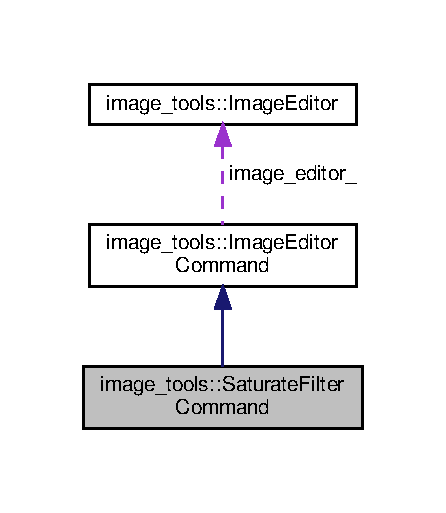
\includegraphics[width=214pt]{classimage__tools_1_1SaturateFilterCommand__coll__graph}
\end{center}
\end{figure}
\subsection*{Public Member Functions}
\begin{DoxyCompactItemize}
\item 
\mbox{\Hypertarget{classimage__tools_1_1SaturateFilterCommand_ac0f09b6034b2925e35db829b42c9ee9e}\label{classimage__tools_1_1SaturateFilterCommand_ac0f09b6034b2925e35db829b42c9ee9e}} 
{\bfseries Saturate\+Filter\+Command} (\hyperlink{classimage__tools_1_1ImageEditor}{Image\+Editor} $\ast$image\+\_\+editor, float scale)
\item 
\mbox{\Hypertarget{classimage__tools_1_1SaturateFilterCommand_a8677cb21e8e951040445713fba0eaa37}\label{classimage__tools_1_1SaturateFilterCommand_a8677cb21e8e951040445713fba0eaa37}} 
void {\bfseries Execute} () override
\end{DoxyCompactItemize}
\subsection*{Additional Inherited Members}


\subsection{Detailed Description}
Specific command for executing a saturate filter. 

The documentation for this class was generated from the following files\+:\begin{DoxyCompactItemize}
\item 
src/mia/image\+\_\+editor\+\_\+commands.\+h\item 
src/mia/image\+\_\+editor\+\_\+commands.\+cc\end{DoxyCompactItemize}

\hypertarget{classimage__tools_1_1SaveCommand}{}\section{image\+\_\+tools\+:\+:Save\+Command Class Reference}
\label{classimage__tools_1_1SaveCommand}\index{image\+\_\+tools\+::\+Save\+Command@{image\+\_\+tools\+::\+Save\+Command}}


{\ttfamily \#include $<$image\+\_\+editor\+\_\+commands.\+h$>$}



Inheritance diagram for image\+\_\+tools\+:\+:Save\+Command\+:
\nopagebreak
\begin{figure}[H]
\begin{center}
\leavevmode
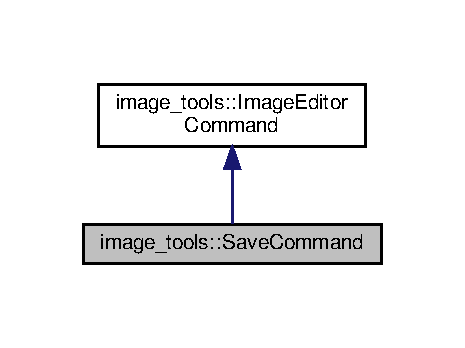
\includegraphics[width=223pt]{classimage__tools_1_1SaveCommand__inherit__graph}
\end{center}
\end{figure}


Collaboration diagram for image\+\_\+tools\+:\+:Save\+Command\+:
\nopagebreak
\begin{figure}[H]
\begin{center}
\leavevmode
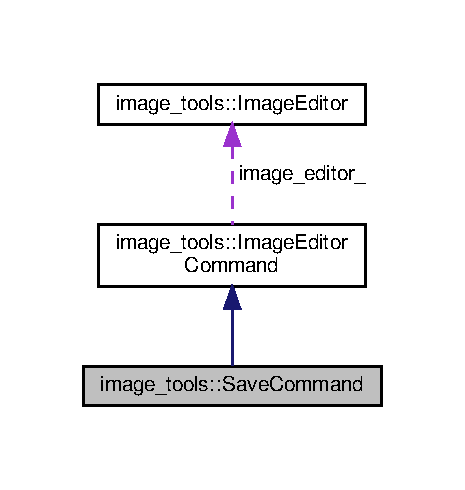
\includegraphics[width=223pt]{classimage__tools_1_1SaveCommand__coll__graph}
\end{center}
\end{figure}
\subsection*{Public Member Functions}
\begin{DoxyCompactItemize}
\item 
\mbox{\Hypertarget{classimage__tools_1_1SaveCommand_a1efb4a2eb98afe5030a06985a958ef6c}\label{classimage__tools_1_1SaveCommand_a1efb4a2eb98afe5030a06985a958ef6c}} 
{\bfseries Save\+Command} (\hyperlink{classimage__tools_1_1ImageEditor}{Image\+Editor} $\ast$image\+\_\+editor, const std\+::string \&filename)
\item 
\mbox{\Hypertarget{classimage__tools_1_1SaveCommand_aec8f2506ee25ce6681c0ba6ab312d10e}\label{classimage__tools_1_1SaveCommand_aec8f2506ee25ce6681c0ba6ab312d10e}} 
void {\bfseries Execute} () override
\end{DoxyCompactItemize}
\subsection*{Additional Inherited Members}


\subsection{Detailed Description}
Specific command for saving a file. 

The documentation for this class was generated from the following files\+:\begin{DoxyCompactItemize}
\item 
src/mia/image\+\_\+editor\+\_\+commands.\+h\item 
src/mia/image\+\_\+editor\+\_\+commands.\+cc\end{DoxyCompactItemize}

\hypertarget{classimage__tools_1_1SharpenFilterCommand}{}\section{image\+\_\+tools\+:\+:Sharpen\+Filter\+Command Class Reference}
\label{classimage__tools_1_1SharpenFilterCommand}\index{image\+\_\+tools\+::\+Sharpen\+Filter\+Command@{image\+\_\+tools\+::\+Sharpen\+Filter\+Command}}


{\ttfamily \#include $<$image\+\_\+editor\+\_\+commands.\+h$>$}



Inheritance diagram for image\+\_\+tools\+:\+:Sharpen\+Filter\+Command\+:
\nopagebreak
\begin{figure}[H]
\begin{center}
\leavevmode
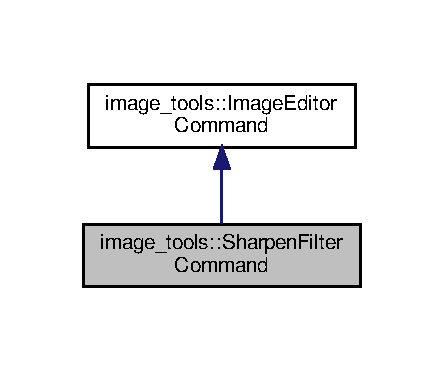
\includegraphics[width=213pt]{classimage__tools_1_1SharpenFilterCommand__inherit__graph}
\end{center}
\end{figure}


Collaboration diagram for image\+\_\+tools\+:\+:Sharpen\+Filter\+Command\+:
\nopagebreak
\begin{figure}[H]
\begin{center}
\leavevmode
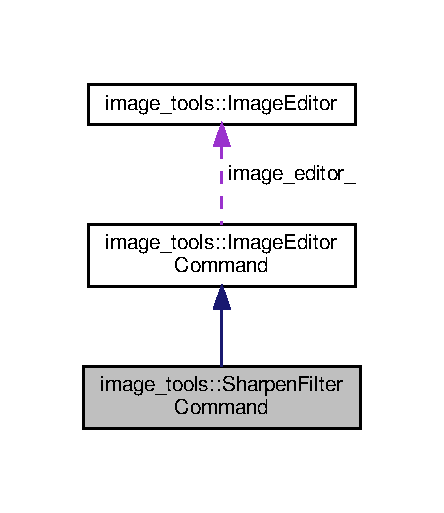
\includegraphics[width=213pt]{classimage__tools_1_1SharpenFilterCommand__coll__graph}
\end{center}
\end{figure}
\subsection*{Public Member Functions}
\begin{DoxyCompactItemize}
\item 
\mbox{\Hypertarget{classimage__tools_1_1SharpenFilterCommand_a819182cc4a326e62c694a9e7741c9aea}\label{classimage__tools_1_1SharpenFilterCommand_a819182cc4a326e62c694a9e7741c9aea}} 
{\bfseries Sharpen\+Filter\+Command} (\hyperlink{classimage__tools_1_1ImageEditor}{Image\+Editor} $\ast$image\+\_\+editor, float radius)
\item 
\mbox{\Hypertarget{classimage__tools_1_1SharpenFilterCommand_a31c1fd39c2495d2888b0644836666ced}\label{classimage__tools_1_1SharpenFilterCommand_a31c1fd39c2495d2888b0644836666ced}} 
void {\bfseries Execute} () override
\end{DoxyCompactItemize}
\subsection*{Additional Inherited Members}


\subsection{Detailed Description}
Specific command for executing a sharpen filter. 

The documentation for this class was generated from the following files\+:\begin{DoxyCompactItemize}
\item 
src/mia/image\+\_\+editor\+\_\+commands.\+h\item 
src/mia/image\+\_\+editor\+\_\+commands.\+cc\end{DoxyCompactItemize}

\hypertarget{classimage__tools_1_1StartStrokeCommand}{}\section{image\+\_\+tools\+:\+:Start\+Stroke\+Command Class Reference}
\label{classimage__tools_1_1StartStrokeCommand}\index{image\+\_\+tools\+::\+Start\+Stroke\+Command@{image\+\_\+tools\+::\+Start\+Stroke\+Command}}


{\ttfamily \#include $<$image\+\_\+editor\+\_\+commands.\+h$>$}



Inheritance diagram for image\+\_\+tools\+:\+:Start\+Stroke\+Command\+:
\nopagebreak
\begin{figure}[H]
\begin{center}
\leavevmode
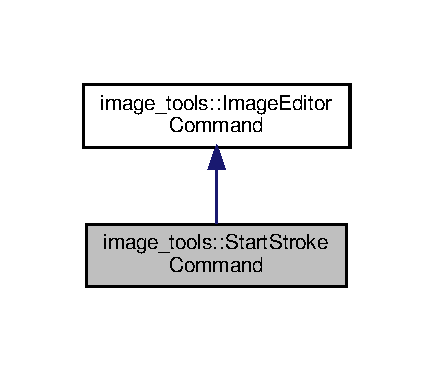
\includegraphics[width=208pt]{classimage__tools_1_1StartStrokeCommand__inherit__graph}
\end{center}
\end{figure}


Collaboration diagram for image\+\_\+tools\+:\+:Start\+Stroke\+Command\+:
\nopagebreak
\begin{figure}[H]
\begin{center}
\leavevmode
\includegraphics[width=208pt]{classimage__tools_1_1StartStrokeCommand__coll__graph}
\end{center}
\end{figure}
\subsection*{Public Member Functions}
\begin{DoxyCompactItemize}
\item 
\mbox{\Hypertarget{classimage__tools_1_1StartStrokeCommand_a93eb3abdeb81243587dcadcad6e6cfe4}\label{classimage__tools_1_1StartStrokeCommand_a93eb3abdeb81243587dcadcad6e6cfe4}} 
{\bfseries Start\+Stroke\+Command} (\hyperlink{classimage__tools_1_1ImageEditor}{Image\+Editor} $\ast$image\+\_\+editor, const std\+::string \&tool\+\_\+name, const \hyperlink{classimage__tools_1_1ColorData}{Color\+Data} \&color, float radius, int x, int y)
\item 
\mbox{\Hypertarget{classimage__tools_1_1StartStrokeCommand_ad4fc2466e4c0370d9437b325ddbd6585}\label{classimage__tools_1_1StartStrokeCommand_ad4fc2466e4c0370d9437b325ddbd6585}} 
void {\bfseries Execute} () override
\end{DoxyCompactItemize}
\subsection*{Additional Inherited Members}


\subsection{Detailed Description}
Specific command for starting a stroke. 

The documentation for this class was generated from the following files\+:\begin{DoxyCompactItemize}
\item 
src/mia/image\+\_\+editor\+\_\+commands.\+h\item 
src/mia/image\+\_\+editor\+\_\+commands.\+cc\end{DoxyCompactItemize}

\hypertarget{classimage__tools_1_1ThresholdFilterCommand}{}\section{image\+\_\+tools\+:\+:Threshold\+Filter\+Command Class Reference}
\label{classimage__tools_1_1ThresholdFilterCommand}\index{image\+\_\+tools\+::\+Threshold\+Filter\+Command@{image\+\_\+tools\+::\+Threshold\+Filter\+Command}}


{\ttfamily \#include $<$image\+\_\+editor\+\_\+commands.\+h$>$}



Inheritance diagram for image\+\_\+tools\+:\+:Threshold\+Filter\+Command\+:
\nopagebreak
\begin{figure}[H]
\begin{center}
\leavevmode
\includegraphics[width=220pt]{classimage__tools_1_1ThresholdFilterCommand__inherit__graph}
\end{center}
\end{figure}


Collaboration diagram for image\+\_\+tools\+:\+:Threshold\+Filter\+Command\+:
\nopagebreak
\begin{figure}[H]
\begin{center}
\leavevmode
\includegraphics[width=220pt]{classimage__tools_1_1ThresholdFilterCommand__coll__graph}
\end{center}
\end{figure}
\subsection*{Public Member Functions}
\begin{DoxyCompactItemize}
\item 
\mbox{\Hypertarget{classimage__tools_1_1ThresholdFilterCommand_ad9c85f7a43fa67c02a0057513e22bcc2}\label{classimage__tools_1_1ThresholdFilterCommand_ad9c85f7a43fa67c02a0057513e22bcc2}} 
{\bfseries Threshold\+Filter\+Command} (\hyperlink{classimage__tools_1_1ImageEditor}{Image\+Editor} $\ast$image\+\_\+editor, float cutoff)
\item 
\mbox{\Hypertarget{classimage__tools_1_1ThresholdFilterCommand_ac8b75145fd088a50a5c0e6412c51a891}\label{classimage__tools_1_1ThresholdFilterCommand_ac8b75145fd088a50a5c0e6412c51a891}} 
void {\bfseries Execute} () override
\end{DoxyCompactItemize}
\subsection*{Additional Inherited Members}


\subsection{Detailed Description}
Specific command for executing a threshold filter. 

The documentation for this class was generated from the following files\+:\begin{DoxyCompactItemize}
\item 
src/mia/image\+\_\+editor\+\_\+commands.\+h\item 
src/mia/image\+\_\+editor\+\_\+commands.\+cc\end{DoxyCompactItemize}

\hypertarget{classimage__tools_1_1Tool}{}\section{image\+\_\+tools\+:\+:Tool Class Reference}
\label{classimage__tools_1_1Tool}\index{image\+\_\+tools\+::\+Tool@{image\+\_\+tools\+::\+Tool}}


{\ttfamily \#include $<$tool.\+h$>$}



Inheritance diagram for image\+\_\+tools\+:\+:Tool\+:
\nopagebreak
\begin{figure}[H]
\begin{center}
\leavevmode
\includegraphics[width=350pt]{classimage__tools_1_1Tool__inherit__graph}
\end{center}
\end{figure}


Collaboration diagram for image\+\_\+tools\+:\+:Tool\+:
\nopagebreak
\begin{figure}[H]
\begin{center}
\leavevmode
\includegraphics[width=350pt]{classimage__tools_1_1Tool__coll__graph}
\end{center}
\end{figure}
\subsection*{Public Member Functions}
\begin{DoxyCompactItemize}
\item 
virtual \hyperlink{classimage__tools_1_1FloatMatrix}{Float\+Matrix} $\ast$ \hyperlink{classimage__tools_1_1Tool_a7d58325846dbc0467e52221daa1310a7}{Create\+Mask} (float radius)=0
\item 
virtual void \hyperlink{classimage__tools_1_1Tool_a1b7cd7d59588923d7e29b6150334f5b8}{Start\+Stroke} (\hyperlink{classimage__tools_1_1PixelBuffer}{Pixel\+Buffer} $\ast$buffer, int x, int y, const \hyperlink{classimage__tools_1_1ColorData}{Color\+Data} \&paint\+\_\+color, float radius)
\item 
virtual void \hyperlink{classimage__tools_1_1Tool_a84d87d7baec8a961be236d4b30636fc0}{Add\+To\+Stroke} (int x, int y)
\item 
void \hyperlink{classimage__tools_1_1Tool_aa76f5cae95ea7cdc30b067b84857a0f5}{End\+Stroke} (int x, int y)
\item 
void \hyperlink{classimage__tools_1_1Tool_a6eb57021e1e59590075411b904e62905}{Stamp\+Mask\+Onto\+Buffer} (int x, int y)
\item 
virtual \hyperlink{classimage__tools_1_1ColorData}{Color\+Data} \hyperlink{classimage__tools_1_1Tool_aaf72d26377a6563fe9002e3288933285}{Lookup\+Paint\+Color} (int x, int y)
\item 
virtual \hyperlink{classimage__tools_1_1ColorData}{Color\+Data} \hyperlink{classimage__tools_1_1Tool_a1f4f417dd13da9ff60481e3e1ff30b69}{Combine\+Paint\+And\+Canvas\+Color} (const \hyperlink{classimage__tools_1_1ColorData}{Color\+Data} \&paint\+\_\+color, const \hyperlink{classimage__tools_1_1ColorData}{Color\+Data} \&canvas\+\_\+color, float mask\+\_\+intensity)
\item 
virtual bool \hyperlink{classimage__tools_1_1Tool_a84b6d2c885d11cf1990a3c7a1343a05f}{applies\+\_\+paint\+\_\+when\+\_\+stationary} ()
\end{DoxyCompactItemize}
\subsection*{Protected Attributes}
\begin{DoxyCompactItemize}
\item 
\mbox{\Hypertarget{classimage__tools_1_1Tool_aaf889880acec7512b12e86ebdbeb3beb}\label{classimage__tools_1_1Tool_aaf889880acec7512b12e86ebdbeb3beb}} 
\hyperlink{classimage__tools_1_1ColorData}{Color\+Data} {\bfseries paint\+\_\+color\+\_\+}
\item 
\mbox{\Hypertarget{classimage__tools_1_1Tool_a23a45a40d69356c9b67ae4302804c28b}\label{classimage__tools_1_1Tool_a23a45a40d69356c9b67ae4302804c28b}} 
\hyperlink{classimage__tools_1_1FloatMatrix}{Float\+Matrix} $\ast$ {\bfseries mask\+\_\+}
\item 
\mbox{\Hypertarget{classimage__tools_1_1Tool_af23788bccb2badbcd03dafeb2b4afb3b}\label{classimage__tools_1_1Tool_af23788bccb2badbcd03dafeb2b4afb3b}} 
\hyperlink{classimage__tools_1_1PixelBuffer}{Pixel\+Buffer} $\ast$ {\bfseries buffer\+\_\+}
\item 
\mbox{\Hypertarget{classimage__tools_1_1Tool_a18f054c5448762db3b1e80bfd7b17510}\label{classimage__tools_1_1Tool_a18f054c5448762db3b1e80bfd7b17510}} 
float {\bfseries stamp\+\_\+overlap\+\_\+}
\item 
\mbox{\Hypertarget{classimage__tools_1_1Tool_ac8354e7948afc34f1a8a85a56a047b76}\label{classimage__tools_1_1Tool_ac8354e7948afc34f1a8a85a56a047b76}} 
int {\bfseries last\+\_\+x\+\_\+}
\item 
\mbox{\Hypertarget{classimage__tools_1_1Tool_a52559a69433d2b4665cd3309751d91ad}\label{classimage__tools_1_1Tool_a52559a69433d2b4665cd3309751d91ad}} 
int {\bfseries last\+\_\+y\+\_\+}
\end{DoxyCompactItemize}


\subsection{Detailed Description}
The base class for an image editing tool. Every tool \char`\"{}has a\char`\"{} mask. Subclasses must define this mask by filling in the Create\+Mask factory method. This base class will then be able to apply the mask to a pixel buffer as the tool is dragged around interactively. 

\subsection{Member Function Documentation}
\mbox{\Hypertarget{classimage__tools_1_1Tool_a84d87d7baec8a961be236d4b30636fc0}\label{classimage__tools_1_1Tool_a84d87d7baec8a961be236d4b30636fc0}} 
\index{image\+\_\+tools\+::\+Tool@{image\+\_\+tools\+::\+Tool}!Add\+To\+Stroke@{Add\+To\+Stroke}}
\index{Add\+To\+Stroke@{Add\+To\+Stroke}!image\+\_\+tools\+::\+Tool@{image\+\_\+tools\+::\+Tool}}
\subsubsection{\texorpdfstring{Add\+To\+Stroke()}{AddToStroke()}}
{\footnotesize\ttfamily void image\+\_\+tools\+::\+Tool\+::\+Add\+To\+Stroke (\begin{DoxyParamCaption}\item[{int}]{x,  }\item[{int}]{y }\end{DoxyParamCaption})\hspace{0.3cm}{\ttfamily [virtual]}}

The controller should call this function after calling \hyperlink{classimage__tools_1_1Tool_a1b7cd7d59588923d7e29b6150334f5b8}{Start\+Stroke()} to add additional line segments to the stroke each time the mouse moves. In other words, each call to \hyperlink{classimage__tools_1_1Tool_a1b7cd7d59588923d7e29b6150334f5b8}{Start\+Stroke()} should by followed by multiple calls to \hyperlink{classimage__tools_1_1Tool_a84d87d7baec8a961be236d4b30636fc0}{Add\+To\+Stroke()}. Keep calling \hyperlink{classimage__tools_1_1Tool_a84d87d7baec8a961be236d4b30636fc0}{Add\+To\+Stroke()} until the user lifts up the mouse button. 

Reimplemented in \hyperlink{classimage__tools_1_1ToolStamp_a098a342f03717e2f909cda9515c85814}{image\+\_\+tools\+::\+Tool\+Stamp}.

\mbox{\Hypertarget{classimage__tools_1_1Tool_a84b6d2c885d11cf1990a3c7a1343a05f}\label{classimage__tools_1_1Tool_a84b6d2c885d11cf1990a3c7a1343a05f}} 
\index{image\+\_\+tools\+::\+Tool@{image\+\_\+tools\+::\+Tool}!applies\+\_\+paint\+\_\+when\+\_\+stationary@{applies\+\_\+paint\+\_\+when\+\_\+stationary}}
\index{applies\+\_\+paint\+\_\+when\+\_\+stationary@{applies\+\_\+paint\+\_\+when\+\_\+stationary}!image\+\_\+tools\+::\+Tool@{image\+\_\+tools\+::\+Tool}}
\subsubsection{\texorpdfstring{applies\+\_\+paint\+\_\+when\+\_\+stationary()}{applies\_paint\_when\_stationary()}}
{\footnotesize\ttfamily bool image\+\_\+tools\+::\+Tool\+::applies\+\_\+paint\+\_\+when\+\_\+stationary (\begin{DoxyParamCaption}{ }\end{DoxyParamCaption})\hspace{0.3cm}{\ttfamily [virtual]}}

Most tools only apply \char`\"{}paint\char`\"{} when they are moved on the canvas, but some, like a spray can continue applying more paint over time even if they are held in the same place. Subclasses should override this function and return true if the tool allows paint to accumulate even when held stationary. The default implmentation returns false. 

Reimplemented in \hyperlink{classimage__tools_1_1ToolSprayCan_acd1e7907873ef757f200bf669d8dbfd9}{image\+\_\+tools\+::\+Tool\+Spray\+Can}.

\mbox{\Hypertarget{classimage__tools_1_1Tool_a1f4f417dd13da9ff60481e3e1ff30b69}\label{classimage__tools_1_1Tool_a1f4f417dd13da9ff60481e3e1ff30b69}} 
\index{image\+\_\+tools\+::\+Tool@{image\+\_\+tools\+::\+Tool}!Combine\+Paint\+And\+Canvas\+Color@{Combine\+Paint\+And\+Canvas\+Color}}
\index{Combine\+Paint\+And\+Canvas\+Color@{Combine\+Paint\+And\+Canvas\+Color}!image\+\_\+tools\+::\+Tool@{image\+\_\+tools\+::\+Tool}}
\subsubsection{\texorpdfstring{Combine\+Paint\+And\+Canvas\+Color()}{CombinePaintAndCanvasColor()}}
{\footnotesize\ttfamily \hyperlink{classimage__tools_1_1ColorData}{Color\+Data} image\+\_\+tools\+::\+Tool\+::\+Combine\+Paint\+And\+Canvas\+Color (\begin{DoxyParamCaption}\item[{const \hyperlink{classimage__tools_1_1ColorData}{Color\+Data} \&}]{paint\+\_\+color,  }\item[{const \hyperlink{classimage__tools_1_1ColorData}{Color\+Data} \&}]{canvas\+\_\+color,  }\item[{float}]{mask\+\_\+intensity }\end{DoxyParamCaption})\hspace{0.3cm}{\ttfamily [virtual]}}

This function combines (i.\+e., blends) a paint\+\_\+color with an underlying canvas\+\_\+color given a mask\+\_\+intensity. The default algorithm uses a standard blending function\+: paint\+\_\+color $\ast$ mask\+\_\+intensity + canvas\+\_\+color $\ast$ (1.\+0 -\/ mask\+\_\+intensity) Some tools require a custom blend. Thus, this function provides a hook for subclasses to override the default blending function. 

Reimplemented in \hyperlink{classimage__tools_1_1ToolHighlighter_a8f4f3c016d4965edd02ad8e8559af4d1}{image\+\_\+tools\+::\+Tool\+Highlighter}, and \hyperlink{classimage__tools_1_1ToolChalk_ab2c6eda363c0fbc2283128eebbd817f5}{image\+\_\+tools\+::\+Tool\+Chalk}.

\mbox{\Hypertarget{classimage__tools_1_1Tool_a7d58325846dbc0467e52221daa1310a7}\label{classimage__tools_1_1Tool_a7d58325846dbc0467e52221daa1310a7}} 
\index{image\+\_\+tools\+::\+Tool@{image\+\_\+tools\+::\+Tool}!Create\+Mask@{Create\+Mask}}
\index{Create\+Mask@{Create\+Mask}!image\+\_\+tools\+::\+Tool@{image\+\_\+tools\+::\+Tool}}
\subsubsection{\texorpdfstring{Create\+Mask()}{CreateMask()}}
{\footnotesize\ttfamily virtual \hyperlink{classimage__tools_1_1FloatMatrix}{Float\+Matrix}$\ast$ image\+\_\+tools\+::\+Tool\+::\+Create\+Mask (\begin{DoxyParamCaption}\item[{float}]{radius }\end{DoxyParamCaption})\hspace{0.3cm}{\ttfamily [pure virtual]}}

Subclasses must fill in this factory method to define the mask for the specific tool they implement. 

Implemented in \hyperlink{classimage__tools_1_1ToolCalligraphyPen_a02a5785e1fabcc142a03509ac50dfb94}{image\+\_\+tools\+::\+Tool\+Calligraphy\+Pen}, \hyperlink{classimage__tools_1_1ToolHighlighter_a8c5c4f6c91fc49a89c1d24bdc2b3ea70}{image\+\_\+tools\+::\+Tool\+Highlighter}, \hyperlink{classimage__tools_1_1ToolStamp_a1331846ac4bcfc7aa307cf966658d056}{image\+\_\+tools\+::\+Tool\+Stamp}, \hyperlink{classimage__tools_1_1ToolBlur_a75690cef3c70c2f8db56b7106d7cd08c}{image\+\_\+tools\+::\+Tool\+Blur}, \hyperlink{classimage__tools_1_1ToolSprayCan_acac77013717667f64c9ffaedf621b553}{image\+\_\+tools\+::\+Tool\+Spray\+Can}, \hyperlink{classimage__tools_1_1ToolChalk_ac5b2bd1d685a80ae4b296defcbc80580}{image\+\_\+tools\+::\+Tool\+Chalk}, \hyperlink{classimage__tools_1_1ToolEraser_a5720244391587679acb8645a3fbd3d63}{image\+\_\+tools\+::\+Tool\+Eraser}, and \hyperlink{classimage__tools_1_1ToolPen_a27237b8843c611f80f59f8c00de4c835}{image\+\_\+tools\+::\+Tool\+Pen}.

\mbox{\Hypertarget{classimage__tools_1_1Tool_aa76f5cae95ea7cdc30b067b84857a0f5}\label{classimage__tools_1_1Tool_aa76f5cae95ea7cdc30b067b84857a0f5}} 
\index{image\+\_\+tools\+::\+Tool@{image\+\_\+tools\+::\+Tool}!End\+Stroke@{End\+Stroke}}
\index{End\+Stroke@{End\+Stroke}!image\+\_\+tools\+::\+Tool@{image\+\_\+tools\+::\+Tool}}
\subsubsection{\texorpdfstring{End\+Stroke()}{EndStroke()}}
{\footnotesize\ttfamily void image\+\_\+tools\+::\+Tool\+::\+End\+Stroke (\begin{DoxyParamCaption}\item[{int}]{x,  }\item[{int}]{y }\end{DoxyParamCaption})}

The controller must call this method to complete the stroke when the user releases the mouse button. \mbox{\Hypertarget{classimage__tools_1_1Tool_aaf72d26377a6563fe9002e3288933285}\label{classimage__tools_1_1Tool_aaf72d26377a6563fe9002e3288933285}} 
\index{image\+\_\+tools\+::\+Tool@{image\+\_\+tools\+::\+Tool}!Lookup\+Paint\+Color@{Lookup\+Paint\+Color}}
\index{Lookup\+Paint\+Color@{Lookup\+Paint\+Color}!image\+\_\+tools\+::\+Tool@{image\+\_\+tools\+::\+Tool}}
\subsubsection{\texorpdfstring{Lookup\+Paint\+Color()}{LookupPaintColor()}}
{\footnotesize\ttfamily \hyperlink{classimage__tools_1_1ColorData}{Color\+Data} image\+\_\+tools\+::\+Tool\+::\+Lookup\+Paint\+Color (\begin{DoxyParamCaption}\item[{int}]{x,  }\item[{int}]{y }\end{DoxyParamCaption})\hspace{0.3cm}{\ttfamily [virtual]}}

This function returns the current paint color used with the tool. In most cases, this is the same as the paint\+\_\+color passed in to the \hyperlink{classimage__tools_1_1Tool_a1b7cd7d59588923d7e29b6150334f5b8}{Start\+Stroke()} function. However, some tools, like the blur tool, have \char`\"{}special paint\char`\"{} that depends on the underlying pixels in the canvas or some other factors. Thus, this function provides a hook for subclasses to override the default paint color to implement special paint colors. 

Reimplemented in \hyperlink{classimage__tools_1_1ToolBlur_af709da063f86da74d878d079fd2aab5e}{image\+\_\+tools\+::\+Tool\+Blur}.

\mbox{\Hypertarget{classimage__tools_1_1Tool_a6eb57021e1e59590075411b904e62905}\label{classimage__tools_1_1Tool_a6eb57021e1e59590075411b904e62905}} 
\index{image\+\_\+tools\+::\+Tool@{image\+\_\+tools\+::\+Tool}!Stamp\+Mask\+Onto\+Buffer@{Stamp\+Mask\+Onto\+Buffer}}
\index{Stamp\+Mask\+Onto\+Buffer@{Stamp\+Mask\+Onto\+Buffer}!image\+\_\+tools\+::\+Tool@{image\+\_\+tools\+::\+Tool}}
\subsubsection{\texorpdfstring{Stamp\+Mask\+Onto\+Buffer()}{StampMaskOntoBuffer()}}
{\footnotesize\ttfamily void image\+\_\+tools\+::\+Tool\+::\+Stamp\+Mask\+Onto\+Buffer (\begin{DoxyParamCaption}\item[{int}]{x,  }\item[{int}]{y }\end{DoxyParamCaption})}

This function will stamp the current mask onto the current buffer exactly one time at a location centered at (x,y) within the buffer. \mbox{\Hypertarget{classimage__tools_1_1Tool_a1b7cd7d59588923d7e29b6150334f5b8}\label{classimage__tools_1_1Tool_a1b7cd7d59588923d7e29b6150334f5b8}} 
\index{image\+\_\+tools\+::\+Tool@{image\+\_\+tools\+::\+Tool}!Start\+Stroke@{Start\+Stroke}}
\index{Start\+Stroke@{Start\+Stroke}!image\+\_\+tools\+::\+Tool@{image\+\_\+tools\+::\+Tool}}
\subsubsection{\texorpdfstring{Start\+Stroke()}{StartStroke()}}
{\footnotesize\ttfamily void image\+\_\+tools\+::\+Tool\+::\+Start\+Stroke (\begin{DoxyParamCaption}\item[{\hyperlink{classimage__tools_1_1PixelBuffer}{Pixel\+Buffer} $\ast$}]{buffer,  }\item[{int}]{x,  }\item[{int}]{y,  }\item[{const \hyperlink{classimage__tools_1_1ColorData}{Color\+Data} \&}]{paint\+\_\+color,  }\item[{float}]{radius }\end{DoxyParamCaption})\hspace{0.3cm}{\ttfamily [virtual]}}

The controller (typically the G\+UI class) must call this method each time the user starts a new stroke. The buffer, paint\+\_\+color, and radius are saved in state variables so that they can be used by subsequent calls to \hyperlink{classimage__tools_1_1Tool_a84d87d7baec8a961be236d4b30636fc0}{Add\+To\+Stroke()} and \hyperlink{classimage__tools_1_1Tool_aa76f5cae95ea7cdc30b067b84857a0f5}{End\+Stroke()}. 

Reimplemented in \hyperlink{classimage__tools_1_1ToolEraser_a5b00cd104c6fb0b34fa3f1f5165ab189}{image\+\_\+tools\+::\+Tool\+Eraser}.



The documentation for this class was generated from the following files\+:\begin{DoxyCompactItemize}
\item 
src/imagetools/tool.\+h\item 
src/imagetools/tool.\+cc\end{DoxyCompactItemize}

\hypertarget{classimage__tools_1_1ToolBlur}{}\section{image\+\_\+tools\+:\+:Tool\+Blur Class Reference}
\label{classimage__tools_1_1ToolBlur}\index{image\+\_\+tools\+::\+Tool\+Blur@{image\+\_\+tools\+::\+Tool\+Blur}}


This tool serves as a mobile version of the blur filter, functions much like the spray can, except with blurring neighboring pixels rather than coloring them (linear falloff).  




{\ttfamily \#include $<$tool\+\_\+blur.\+h$>$}



Inheritance diagram for image\+\_\+tools\+:\+:Tool\+Blur\+:
\nopagebreak
\begin{figure}[H]
\begin{center}
\leavevmode
\includegraphics[width=191pt]{classimage__tools_1_1ToolBlur__inherit__graph}
\end{center}
\end{figure}


Collaboration diagram for image\+\_\+tools\+:\+:Tool\+Blur\+:
\nopagebreak
\begin{figure}[H]
\begin{center}
\leavevmode
\includegraphics[width=350pt]{classimage__tools_1_1ToolBlur__coll__graph}
\end{center}
\end{figure}
\subsection*{Public Member Functions}
\begin{DoxyCompactItemize}
\item 
\hyperlink{classimage__tools_1_1FloatMatrix}{Float\+Matrix} $\ast$ \hyperlink{classimage__tools_1_1ToolBlur_a75690cef3c70c2f8db56b7106d7cd08c}{Create\+Mask} (float radius) override
\item 
\hyperlink{classimage__tools_1_1ColorData}{Color\+Data} \hyperlink{classimage__tools_1_1ToolBlur_af709da063f86da74d878d079fd2aab5e}{Lookup\+Paint\+Color} (int x, int y) override
\end{DoxyCompactItemize}
\subsection*{Static Public Member Functions}
\begin{DoxyCompactItemize}
\item 
\mbox{\Hypertarget{classimage__tools_1_1ToolBlur_a8faee980a676d32430a6e7440e929ce6}\label{classimage__tools_1_1ToolBlur_a8faee980a676d32430a6e7440e929ce6}} 
static const std\+::string {\bfseries name} ()
\end{DoxyCompactItemize}
\subsection*{Additional Inherited Members}


\subsection{Detailed Description}
This tool serves as a mobile version of the blur filter, functions much like the spray can, except with blurring neighboring pixels rather than coloring them (linear falloff). 

\subsection{Member Function Documentation}
\mbox{\Hypertarget{classimage__tools_1_1ToolBlur_a75690cef3c70c2f8db56b7106d7cd08c}\label{classimage__tools_1_1ToolBlur_a75690cef3c70c2f8db56b7106d7cd08c}} 
\index{image\+\_\+tools\+::\+Tool\+Blur@{image\+\_\+tools\+::\+Tool\+Blur}!Create\+Mask@{Create\+Mask}}
\index{Create\+Mask@{Create\+Mask}!image\+\_\+tools\+::\+Tool\+Blur@{image\+\_\+tools\+::\+Tool\+Blur}}
\subsubsection{\texorpdfstring{Create\+Mask()}{CreateMask()}}
{\footnotesize\ttfamily \hyperlink{classimage__tools_1_1FloatMatrix}{Float\+Matrix} $\ast$ image\+\_\+tools\+::\+Tool\+Blur\+::\+Create\+Mask (\begin{DoxyParamCaption}\item[{float}]{radius }\end{DoxyParamCaption})\hspace{0.3cm}{\ttfamily [override]}, {\ttfamily [virtual]}}

Subclasses must fill in this factory method to define the mask for the specific tool they implement. 

Implements \hyperlink{classimage__tools_1_1Tool_a7d58325846dbc0467e52221daa1310a7}{image\+\_\+tools\+::\+Tool}.

\mbox{\Hypertarget{classimage__tools_1_1ToolBlur_af709da063f86da74d878d079fd2aab5e}\label{classimage__tools_1_1ToolBlur_af709da063f86da74d878d079fd2aab5e}} 
\index{image\+\_\+tools\+::\+Tool\+Blur@{image\+\_\+tools\+::\+Tool\+Blur}!Lookup\+Paint\+Color@{Lookup\+Paint\+Color}}
\index{Lookup\+Paint\+Color@{Lookup\+Paint\+Color}!image\+\_\+tools\+::\+Tool\+Blur@{image\+\_\+tools\+::\+Tool\+Blur}}
\subsubsection{\texorpdfstring{Lookup\+Paint\+Color()}{LookupPaintColor()}}
{\footnotesize\ttfamily \hyperlink{classimage__tools_1_1ColorData}{Color\+Data} image\+\_\+tools\+::\+Tool\+Blur\+::\+Lookup\+Paint\+Color (\begin{DoxyParamCaption}\item[{int}]{x,  }\item[{int}]{y }\end{DoxyParamCaption})\hspace{0.3cm}{\ttfamily [override]}, {\ttfamily [virtual]}}

This function returns the current paint color used with the tool. In most cases, this is the same as the paint\+\_\+color passed in to the \hyperlink{classimage__tools_1_1Tool_a1b7cd7d59588923d7e29b6150334f5b8}{Start\+Stroke()} function. However, some tools, like the blur tool, have \char`\"{}special paint\char`\"{} that depends on the underlying pixels in the canvas or some other factors. Thus, this function provides a hook for subclasses to override the default paint color to implement special paint colors. 

Reimplemented from \hyperlink{classimage__tools_1_1Tool_aaf72d26377a6563fe9002e3288933285}{image\+\_\+tools\+::\+Tool}.



The documentation for this class was generated from the following files\+:\begin{DoxyCompactItemize}
\item 
src/imagetools/tool\+\_\+blur.\+h\item 
src/imagetools/tool\+\_\+blur.\+cc\end{DoxyCompactItemize}

\hypertarget{classimage__tools_1_1ToolCalligraphyPen}{}\section{image\+\_\+tools\+:\+:Tool\+Calligraphy\+Pen Class Reference}
\label{classimage__tools_1_1ToolCalligraphyPen}\index{image\+\_\+tools\+::\+Tool\+Calligraphy\+Pen@{image\+\_\+tools\+::\+Tool\+Calligraphy\+Pen}}


This tool simulates a Calligraphy Pen, meaning it paints with a different thickness depending on which direction it is moved. It has a oval mask tilted at an angle of 70 degrees counter-\/clockwise from the x-\/axis and an elongation ratio of 0.\+333.  




{\ttfamily \#include $<$tool\+\_\+calligraphy\+\_\+pen.\+h$>$}



Inheritance diagram for image\+\_\+tools\+:\+:Tool\+Calligraphy\+Pen\+:
\nopagebreak
\begin{figure}[H]
\begin{center}
\leavevmode
\includegraphics[width=240pt]{classimage__tools_1_1ToolCalligraphyPen__inherit__graph}
\end{center}
\end{figure}


Collaboration diagram for image\+\_\+tools\+:\+:Tool\+Calligraphy\+Pen\+:
\nopagebreak
\begin{figure}[H]
\begin{center}
\leavevmode
\includegraphics[width=350pt]{classimage__tools_1_1ToolCalligraphyPen__coll__graph}
\end{center}
\end{figure}
\subsection*{Public Member Functions}
\begin{DoxyCompactItemize}
\item 
\hyperlink{classimage__tools_1_1FloatMatrix}{Float\+Matrix} $\ast$ \hyperlink{classimage__tools_1_1ToolCalligraphyPen_a02a5785e1fabcc142a03509ac50dfb94}{Create\+Mask} (float radius) override
\end{DoxyCompactItemize}
\subsection*{Static Public Member Functions}
\begin{DoxyCompactItemize}
\item 
\mbox{\Hypertarget{classimage__tools_1_1ToolCalligraphyPen_acba5aa1019ec3c48cc3a3854e0e5bf55}\label{classimage__tools_1_1ToolCalligraphyPen_acba5aa1019ec3c48cc3a3854e0e5bf55}} 
static const std\+::string {\bfseries name} ()
\end{DoxyCompactItemize}
\subsection*{Additional Inherited Members}


\subsection{Detailed Description}
This tool simulates a Calligraphy Pen, meaning it paints with a different thickness depending on which direction it is moved. It has a oval mask tilted at an angle of 70 degrees counter-\/clockwise from the x-\/axis and an elongation ratio of 0.\+333. 

\subsection{Member Function Documentation}
\mbox{\Hypertarget{classimage__tools_1_1ToolCalligraphyPen_a02a5785e1fabcc142a03509ac50dfb94}\label{classimage__tools_1_1ToolCalligraphyPen_a02a5785e1fabcc142a03509ac50dfb94}} 
\index{image\+\_\+tools\+::\+Tool\+Calligraphy\+Pen@{image\+\_\+tools\+::\+Tool\+Calligraphy\+Pen}!Create\+Mask@{Create\+Mask}}
\index{Create\+Mask@{Create\+Mask}!image\+\_\+tools\+::\+Tool\+Calligraphy\+Pen@{image\+\_\+tools\+::\+Tool\+Calligraphy\+Pen}}
\subsubsection{\texorpdfstring{Create\+Mask()}{CreateMask()}}
{\footnotesize\ttfamily \hyperlink{classimage__tools_1_1FloatMatrix}{Float\+Matrix} $\ast$ image\+\_\+tools\+::\+Tool\+Calligraphy\+Pen\+::\+Create\+Mask (\begin{DoxyParamCaption}\item[{float}]{radius }\end{DoxyParamCaption})\hspace{0.3cm}{\ttfamily [override]}, {\ttfamily [virtual]}}

Subclasses must fill in this factory method to define the mask for the specific tool they implement. 

Implements \hyperlink{classimage__tools_1_1Tool_a7d58325846dbc0467e52221daa1310a7}{image\+\_\+tools\+::\+Tool}.



The documentation for this class was generated from the following files\+:\begin{DoxyCompactItemize}
\item 
src/imagetools/tool\+\_\+calligraphy\+\_\+pen.\+h\item 
src/imagetools/tool\+\_\+calligraphy\+\_\+pen.\+cc\end{DoxyCompactItemize}

\hypertarget{classimage__tools_1_1ToolChalk}{}\section{image\+\_\+tools\+:\+:Tool\+Chalk Class Reference}
\label{classimage__tools_1_1ToolChalk}\index{image\+\_\+tools\+::\+Tool\+Chalk@{image\+\_\+tools\+::\+Tool\+Chalk}}


This tool simulates chalk drawing on a rough paper. The class overrides \hyperlink{classimage__tools_1_1Tool}{Tool}\textquotesingle{}s default color blending function to insert random noise as the tool is moved around.  




{\ttfamily \#include $<$tool\+\_\+chalk.\+h$>$}



Inheritance diagram for image\+\_\+tools\+:\+:Tool\+Chalk\+:
\nopagebreak
\begin{figure}[H]
\begin{center}
\leavevmode
\includegraphics[width=199pt]{classimage__tools_1_1ToolChalk__inherit__graph}
\end{center}
\end{figure}


Collaboration diagram for image\+\_\+tools\+:\+:Tool\+Chalk\+:
\nopagebreak
\begin{figure}[H]
\begin{center}
\leavevmode
\includegraphics[width=350pt]{classimage__tools_1_1ToolChalk__coll__graph}
\end{center}
\end{figure}
\subsection*{Public Member Functions}
\begin{DoxyCompactItemize}
\item 
\hyperlink{classimage__tools_1_1FloatMatrix}{Float\+Matrix} $\ast$ \hyperlink{classimage__tools_1_1ToolChalk_ac5b2bd1d685a80ae4b296defcbc80580}{Create\+Mask} (float radius) override
\item 
\hyperlink{classimage__tools_1_1ColorData}{Color\+Data} \hyperlink{classimage__tools_1_1ToolChalk_ab2c6eda363c0fbc2283128eebbd817f5}{Combine\+Paint\+And\+Canvas\+Color} (const \hyperlink{classimage__tools_1_1ColorData}{Color\+Data} \&paint\+\_\+color, const \hyperlink{classimage__tools_1_1ColorData}{Color\+Data} \&canvas\+\_\+color, float mask\+\_\+intensity) override
\end{DoxyCompactItemize}
\subsection*{Static Public Member Functions}
\begin{DoxyCompactItemize}
\item 
\mbox{\Hypertarget{classimage__tools_1_1ToolChalk_a8304555902b7708bab24821d355b3ff0}\label{classimage__tools_1_1ToolChalk_a8304555902b7708bab24821d355b3ff0}} 
static const std\+::string {\bfseries name} ()
\end{DoxyCompactItemize}
\subsection*{Additional Inherited Members}


\subsection{Detailed Description}
This tool simulates chalk drawing on a rough paper. The class overrides \hyperlink{classimage__tools_1_1Tool}{Tool}\textquotesingle{}s default color blending function to insert random noise as the tool is moved around. 

\subsection{Member Function Documentation}
\mbox{\Hypertarget{classimage__tools_1_1ToolChalk_ab2c6eda363c0fbc2283128eebbd817f5}\label{classimage__tools_1_1ToolChalk_ab2c6eda363c0fbc2283128eebbd817f5}} 
\index{image\+\_\+tools\+::\+Tool\+Chalk@{image\+\_\+tools\+::\+Tool\+Chalk}!Combine\+Paint\+And\+Canvas\+Color@{Combine\+Paint\+And\+Canvas\+Color}}
\index{Combine\+Paint\+And\+Canvas\+Color@{Combine\+Paint\+And\+Canvas\+Color}!image\+\_\+tools\+::\+Tool\+Chalk@{image\+\_\+tools\+::\+Tool\+Chalk}}
\subsubsection{\texorpdfstring{Combine\+Paint\+And\+Canvas\+Color()}{CombinePaintAndCanvasColor()}}
{\footnotesize\ttfamily \hyperlink{classimage__tools_1_1ColorData}{Color\+Data} image\+\_\+tools\+::\+Tool\+Chalk\+::\+Combine\+Paint\+And\+Canvas\+Color (\begin{DoxyParamCaption}\item[{const \hyperlink{classimage__tools_1_1ColorData}{Color\+Data} \&}]{paint\+\_\+color,  }\item[{const \hyperlink{classimage__tools_1_1ColorData}{Color\+Data} \&}]{canvas\+\_\+color,  }\item[{float}]{mask\+\_\+intensity }\end{DoxyParamCaption})\hspace{0.3cm}{\ttfamily [override]}, {\ttfamily [virtual]}}

This function combines (i.\+e., blends) a paint\+\_\+color with an underlying canvas\+\_\+color given a mask\+\_\+intensity. The default algorithm uses a standard blending function\+: paint\+\_\+color $\ast$ mask\+\_\+intensity + canvas\+\_\+color $\ast$ (1.\+0 -\/ mask\+\_\+intensity) Some tools require a custom blend. Thus, this function provides a hook for subclasses to override the default blending function. 

Reimplemented from \hyperlink{classimage__tools_1_1Tool_a1f4f417dd13da9ff60481e3e1ff30b69}{image\+\_\+tools\+::\+Tool}.

\mbox{\Hypertarget{classimage__tools_1_1ToolChalk_ac5b2bd1d685a80ae4b296defcbc80580}\label{classimage__tools_1_1ToolChalk_ac5b2bd1d685a80ae4b296defcbc80580}} 
\index{image\+\_\+tools\+::\+Tool\+Chalk@{image\+\_\+tools\+::\+Tool\+Chalk}!Create\+Mask@{Create\+Mask}}
\index{Create\+Mask@{Create\+Mask}!image\+\_\+tools\+::\+Tool\+Chalk@{image\+\_\+tools\+::\+Tool\+Chalk}}
\subsubsection{\texorpdfstring{Create\+Mask()}{CreateMask()}}
{\footnotesize\ttfamily \hyperlink{classimage__tools_1_1FloatMatrix}{Float\+Matrix} $\ast$ image\+\_\+tools\+::\+Tool\+Chalk\+::\+Create\+Mask (\begin{DoxyParamCaption}\item[{float}]{radius }\end{DoxyParamCaption})\hspace{0.3cm}{\ttfamily [override]}, {\ttfamily [virtual]}}

Subclasses must fill in this factory method to define the mask for the specific tool they implement. 

Implements \hyperlink{classimage__tools_1_1Tool_a7d58325846dbc0467e52221daa1310a7}{image\+\_\+tools\+::\+Tool}.



The documentation for this class was generated from the following files\+:\begin{DoxyCompactItemize}
\item 
src/imagetools/tool\+\_\+chalk.\+h\item 
src/imagetools/tool\+\_\+chalk.\+cc\end{DoxyCompactItemize}

\hypertarget{classimage__tools_1_1ToolEraser}{}\section{image\+\_\+tools\+:\+:Tool\+Eraser Class Reference}
\label{classimage__tools_1_1ToolEraser}\index{image\+\_\+tools\+::\+Tool\+Eraser@{image\+\_\+tools\+::\+Tool\+Eraser}}


This tool simulates an Eraser. It overrides the \hyperlink{classimage__tools_1_1Tool}{Tool}\textquotesingle{}s Start\+Stroke method to change the paint\+\_\+color to be the canvas\textquotesingle{}s background color.  




{\ttfamily \#include $<$tool\+\_\+eraser.\+h$>$}



Inheritance diagram for image\+\_\+tools\+:\+:Tool\+Eraser\+:
\nopagebreak
\begin{figure}[H]
\begin{center}
\leavevmode
\includegraphics[width=202pt]{classimage__tools_1_1ToolEraser__inherit__graph}
\end{center}
\end{figure}


Collaboration diagram for image\+\_\+tools\+:\+:Tool\+Eraser\+:
\nopagebreak
\begin{figure}[H]
\begin{center}
\leavevmode
\includegraphics[width=350pt]{classimage__tools_1_1ToolEraser__coll__graph}
\end{center}
\end{figure}
\subsection*{Public Member Functions}
\begin{DoxyCompactItemize}
\item 
\hyperlink{classimage__tools_1_1FloatMatrix}{Float\+Matrix} $\ast$ \hyperlink{classimage__tools_1_1ToolEraser_a5720244391587679acb8645a3fbd3d63}{Create\+Mask} (float radius) override
\item 
void \hyperlink{classimage__tools_1_1ToolEraser_a5b00cd104c6fb0b34fa3f1f5165ab189}{Start\+Stroke} (\hyperlink{classimage__tools_1_1PixelBuffer}{Pixel\+Buffer} $\ast$buffer, int x, int y, const \hyperlink{classimage__tools_1_1ColorData}{Color\+Data} \&paint\+\_\+color, float radius) override
\end{DoxyCompactItemize}
\subsection*{Static Public Member Functions}
\begin{DoxyCompactItemize}
\item 
\mbox{\Hypertarget{classimage__tools_1_1ToolEraser_a95d93a6bb8ab437f44f4846c6d08c74f}\label{classimage__tools_1_1ToolEraser_a95d93a6bb8ab437f44f4846c6d08c74f}} 
static const std\+::string {\bfseries name} ()
\end{DoxyCompactItemize}
\subsection*{Additional Inherited Members}


\subsection{Detailed Description}
This tool simulates an Eraser. It overrides the \hyperlink{classimage__tools_1_1Tool}{Tool}\textquotesingle{}s Start\+Stroke method to change the paint\+\_\+color to be the canvas\textquotesingle{}s background color. 

\subsection{Member Function Documentation}
\mbox{\Hypertarget{classimage__tools_1_1ToolEraser_a5720244391587679acb8645a3fbd3d63}\label{classimage__tools_1_1ToolEraser_a5720244391587679acb8645a3fbd3d63}} 
\index{image\+\_\+tools\+::\+Tool\+Eraser@{image\+\_\+tools\+::\+Tool\+Eraser}!Create\+Mask@{Create\+Mask}}
\index{Create\+Mask@{Create\+Mask}!image\+\_\+tools\+::\+Tool\+Eraser@{image\+\_\+tools\+::\+Tool\+Eraser}}
\subsubsection{\texorpdfstring{Create\+Mask()}{CreateMask()}}
{\footnotesize\ttfamily \hyperlink{classimage__tools_1_1FloatMatrix}{Float\+Matrix} $\ast$ image\+\_\+tools\+::\+Tool\+Eraser\+::\+Create\+Mask (\begin{DoxyParamCaption}\item[{float}]{radius }\end{DoxyParamCaption})\hspace{0.3cm}{\ttfamily [override]}, {\ttfamily [virtual]}}

Subclasses must fill in this factory method to define the mask for the specific tool they implement. 

Implements \hyperlink{classimage__tools_1_1Tool_a7d58325846dbc0467e52221daa1310a7}{image\+\_\+tools\+::\+Tool}.

\mbox{\Hypertarget{classimage__tools_1_1ToolEraser_a5b00cd104c6fb0b34fa3f1f5165ab189}\label{classimage__tools_1_1ToolEraser_a5b00cd104c6fb0b34fa3f1f5165ab189}} 
\index{image\+\_\+tools\+::\+Tool\+Eraser@{image\+\_\+tools\+::\+Tool\+Eraser}!Start\+Stroke@{Start\+Stroke}}
\index{Start\+Stroke@{Start\+Stroke}!image\+\_\+tools\+::\+Tool\+Eraser@{image\+\_\+tools\+::\+Tool\+Eraser}}
\subsubsection{\texorpdfstring{Start\+Stroke()}{StartStroke()}}
{\footnotesize\ttfamily void image\+\_\+tools\+::\+Tool\+Eraser\+::\+Start\+Stroke (\begin{DoxyParamCaption}\item[{\hyperlink{classimage__tools_1_1PixelBuffer}{Pixel\+Buffer} $\ast$}]{buffer,  }\item[{int}]{x,  }\item[{int}]{y,  }\item[{const \hyperlink{classimage__tools_1_1ColorData}{Color\+Data} \&}]{paint\+\_\+color,  }\item[{float}]{radius }\end{DoxyParamCaption})\hspace{0.3cm}{\ttfamily [override]}, {\ttfamily [virtual]}}

The controller (typically the G\+UI class) must call this method each time the user starts a new stroke. The buffer, paint\+\_\+color, and radius are saved in state variables so that they can be used by subsequent calls to \hyperlink{classimage__tools_1_1Tool_a84d87d7baec8a961be236d4b30636fc0}{Add\+To\+Stroke()} and \hyperlink{classimage__tools_1_1Tool_aa76f5cae95ea7cdc30b067b84857a0f5}{End\+Stroke()}. 

Reimplemented from \hyperlink{classimage__tools_1_1Tool_a1b7cd7d59588923d7e29b6150334f5b8}{image\+\_\+tools\+::\+Tool}.



The documentation for this class was generated from the following files\+:\begin{DoxyCompactItemize}
\item 
src/imagetools/tool\+\_\+eraser.\+h\item 
src/imagetools/tool\+\_\+eraser.\+cc\end{DoxyCompactItemize}

\hypertarget{classimage__tools_1_1ToolHighlighter}{}\section{image\+\_\+tools\+:\+:Tool\+Highlighter Class Reference}
\label{classimage__tools_1_1ToolHighlighter}\index{image\+\_\+tools\+::\+Tool\+Highlighter@{image\+\_\+tools\+::\+Tool\+Highlighter}}


This tool simulates a Highlighter. It has a semi-\/transparent oval mask. It overrides the default \hyperlink{classimage__tools_1_1Tool}{Tool}\textquotesingle{}s color blend function to make the blending dependent upon the luminance of the underlying canvas color.  




{\ttfamily \#include $<$tool\+\_\+highlighter.\+h$>$}



Inheritance diagram for image\+\_\+tools\+:\+:Tool\+Highlighter\+:
\nopagebreak
\begin{figure}[H]
\begin{center}
\leavevmode
\includegraphics[width=220pt]{classimage__tools_1_1ToolHighlighter__inherit__graph}
\end{center}
\end{figure}


Collaboration diagram for image\+\_\+tools\+:\+:Tool\+Highlighter\+:
\nopagebreak
\begin{figure}[H]
\begin{center}
\leavevmode
\includegraphics[width=350pt]{classimage__tools_1_1ToolHighlighter__coll__graph}
\end{center}
\end{figure}
\subsection*{Public Member Functions}
\begin{DoxyCompactItemize}
\item 
\hyperlink{classimage__tools_1_1FloatMatrix}{Float\+Matrix} $\ast$ \hyperlink{classimage__tools_1_1ToolHighlighter_a8c5c4f6c91fc49a89c1d24bdc2b3ea70}{Create\+Mask} (float radius) override
\item 
\mbox{\Hypertarget{classimage__tools_1_1ToolHighlighter_a8f4f3c016d4965edd02ad8e8559af4d1}\label{classimage__tools_1_1ToolHighlighter_a8f4f3c016d4965edd02ad8e8559af4d1}} 
\hyperlink{classimage__tools_1_1ColorData}{Color\+Data} \hyperlink{classimage__tools_1_1ToolHighlighter_a8f4f3c016d4965edd02ad8e8559af4d1}{Combine\+Paint\+And\+Canvas\+Color} (const \hyperlink{classimage__tools_1_1ColorData}{Color\+Data} \&paint\+\_\+color, const \hyperlink{classimage__tools_1_1ColorData}{Color\+Data} \&canvas\+\_\+color, float mask\+\_\+intensity) override
\begin{DoxyCompactList}\small\item\em Overrides the super\textquotesingle{}s function to include the luminance of the canvas\+\_\+color in the calculation of the tool\textquotesingle{}s intensity. \end{DoxyCompactList}\end{DoxyCompactItemize}
\subsection*{Static Public Member Functions}
\begin{DoxyCompactItemize}
\item 
\mbox{\Hypertarget{classimage__tools_1_1ToolHighlighter_ae55632ec3524f34bc7c0c3238d03b6c0}\label{classimage__tools_1_1ToolHighlighter_ae55632ec3524f34bc7c0c3238d03b6c0}} 
static const std\+::string {\bfseries name} ()
\end{DoxyCompactItemize}
\subsection*{Additional Inherited Members}


\subsection{Detailed Description}
This tool simulates a Highlighter. It has a semi-\/transparent oval mask. It overrides the default \hyperlink{classimage__tools_1_1Tool}{Tool}\textquotesingle{}s color blend function to make the blending dependent upon the luminance of the underlying canvas color. 

\subsection{Member Function Documentation}
\mbox{\Hypertarget{classimage__tools_1_1ToolHighlighter_a8c5c4f6c91fc49a89c1d24bdc2b3ea70}\label{classimage__tools_1_1ToolHighlighter_a8c5c4f6c91fc49a89c1d24bdc2b3ea70}} 
\index{image\+\_\+tools\+::\+Tool\+Highlighter@{image\+\_\+tools\+::\+Tool\+Highlighter}!Create\+Mask@{Create\+Mask}}
\index{Create\+Mask@{Create\+Mask}!image\+\_\+tools\+::\+Tool\+Highlighter@{image\+\_\+tools\+::\+Tool\+Highlighter}}
\subsubsection{\texorpdfstring{Create\+Mask()}{CreateMask()}}
{\footnotesize\ttfamily \hyperlink{classimage__tools_1_1FloatMatrix}{Float\+Matrix} $\ast$ image\+\_\+tools\+::\+Tool\+Highlighter\+::\+Create\+Mask (\begin{DoxyParamCaption}\item[{float}]{radius }\end{DoxyParamCaption})\hspace{0.3cm}{\ttfamily [override]}, {\ttfamily [virtual]}}

Subclasses must fill in this factory method to define the mask for the specific tool they implement. 

Implements \hyperlink{classimage__tools_1_1Tool_a7d58325846dbc0467e52221daa1310a7}{image\+\_\+tools\+::\+Tool}.



The documentation for this class was generated from the following files\+:\begin{DoxyCompactItemize}
\item 
src/imagetools/tool\+\_\+highlighter.\+h\item 
src/imagetools/tool\+\_\+highlighter.\+cc\end{DoxyCompactItemize}

\hypertarget{classimage__tools_1_1ToolPen}{}\section{image\+\_\+tools\+:\+:Tool\+Pen Class Reference}
\label{classimage__tools_1_1ToolPen}\index{image\+\_\+tools\+::\+Tool\+Pen@{image\+\_\+tools\+::\+Tool\+Pen}}


The simplest of tools, this has a mask that is a completely opaque circle.  




{\ttfamily \#include $<$tool\+\_\+pen.\+h$>$}



Inheritance diagram for image\+\_\+tools\+:\+:Tool\+Pen\+:
\nopagebreak
\begin{figure}[H]
\begin{center}
\leavevmode
\includegraphics[width=191pt]{classimage__tools_1_1ToolPen__inherit__graph}
\end{center}
\end{figure}


Collaboration diagram for image\+\_\+tools\+:\+:Tool\+Pen\+:
\nopagebreak
\begin{figure}[H]
\begin{center}
\leavevmode
\includegraphics[width=350pt]{classimage__tools_1_1ToolPen__coll__graph}
\end{center}
\end{figure}
\subsection*{Public Member Functions}
\begin{DoxyCompactItemize}
\item 
\hyperlink{classimage__tools_1_1FloatMatrix}{Float\+Matrix} $\ast$ \hyperlink{classimage__tools_1_1ToolPen_a27237b8843c611f80f59f8c00de4c835}{Create\+Mask} (float radius) override
\end{DoxyCompactItemize}
\subsection*{Static Public Member Functions}
\begin{DoxyCompactItemize}
\item 
\mbox{\Hypertarget{classimage__tools_1_1ToolPen_aa5a82e88e162d8db4600139b8740c27b}\label{classimage__tools_1_1ToolPen_aa5a82e88e162d8db4600139b8740c27b}} 
static const std\+::string {\bfseries name} ()
\end{DoxyCompactItemize}
\subsection*{Additional Inherited Members}


\subsection{Detailed Description}
The simplest of tools, this has a mask that is a completely opaque circle. 

\subsection{Member Function Documentation}
\mbox{\Hypertarget{classimage__tools_1_1ToolPen_a27237b8843c611f80f59f8c00de4c835}\label{classimage__tools_1_1ToolPen_a27237b8843c611f80f59f8c00de4c835}} 
\index{image\+\_\+tools\+::\+Tool\+Pen@{image\+\_\+tools\+::\+Tool\+Pen}!Create\+Mask@{Create\+Mask}}
\index{Create\+Mask@{Create\+Mask}!image\+\_\+tools\+::\+Tool\+Pen@{image\+\_\+tools\+::\+Tool\+Pen}}
\subsubsection{\texorpdfstring{Create\+Mask()}{CreateMask()}}
{\footnotesize\ttfamily \hyperlink{classimage__tools_1_1FloatMatrix}{Float\+Matrix} $\ast$ image\+\_\+tools\+::\+Tool\+Pen\+::\+Create\+Mask (\begin{DoxyParamCaption}\item[{float}]{radius }\end{DoxyParamCaption})\hspace{0.3cm}{\ttfamily [override]}, {\ttfamily [virtual]}}

Subclasses must fill in this factory method to define the mask for the specific tool they implement. 

Implements \hyperlink{classimage__tools_1_1Tool_a7d58325846dbc0467e52221daa1310a7}{image\+\_\+tools\+::\+Tool}.



The documentation for this class was generated from the following files\+:\begin{DoxyCompactItemize}
\item 
src/imagetools/tool\+\_\+pen.\+h\item 
src/imagetools/tool\+\_\+pen.\+cc\end{DoxyCompactItemize}

\hypertarget{classimage__tools_1_1ToolSprayCan}{}\section{image\+\_\+tools\+:\+:Tool\+Spray\+Can Class Reference}
\label{classimage__tools_1_1ToolSprayCan}\index{image\+\_\+tools\+::\+Tool\+Spray\+Can@{image\+\_\+tools\+::\+Tool\+Spray\+Can}}


{\ttfamily \#include $<$tool\+\_\+spray\+\_\+can.\+h$>$}



Inheritance diagram for image\+\_\+tools\+:\+:Tool\+Spray\+Can\+:
\nopagebreak
\begin{figure}[H]
\begin{center}
\leavevmode
\includegraphics[width=217pt]{classimage__tools_1_1ToolSprayCan__inherit__graph}
\end{center}
\end{figure}


Collaboration diagram for image\+\_\+tools\+:\+:Tool\+Spray\+Can\+:
\nopagebreak
\begin{figure}[H]
\begin{center}
\leavevmode
\includegraphics[width=350pt]{classimage__tools_1_1ToolSprayCan__coll__graph}
\end{center}
\end{figure}
\subsection*{Public Member Functions}
\begin{DoxyCompactItemize}
\item 
\hyperlink{classimage__tools_1_1FloatMatrix}{Float\+Matrix} $\ast$ \hyperlink{classimage__tools_1_1ToolSprayCan_acac77013717667f64c9ffaedf621b553}{Create\+Mask} (float radius) override
\item 
bool \hyperlink{classimage__tools_1_1ToolSprayCan_acd1e7907873ef757f200bf669d8dbfd9}{applies\+\_\+paint\+\_\+when\+\_\+stationary} () override
\end{DoxyCompactItemize}
\subsection*{Static Public Member Functions}
\begin{DoxyCompactItemize}
\item 
\mbox{\Hypertarget{classimage__tools_1_1ToolSprayCan_af0beec74bf6527306e67688445571c29}\label{classimage__tools_1_1ToolSprayCan_af0beec74bf6527306e67688445571c29}} 
static const std\+::string {\bfseries name} ()
\end{DoxyCompactItemize}
\subsection*{Additional Inherited Members}


\subsection{Detailed Description}
This tool has a linear falloff so that it looks like the paint has been sprayed onto the canvas. It also has the interesting property that it continues to paint even when held stationary so paint continues to accumulate on the canvas the longer you hold it still. 

\subsection{Member Function Documentation}
\mbox{\Hypertarget{classimage__tools_1_1ToolSprayCan_acd1e7907873ef757f200bf669d8dbfd9}\label{classimage__tools_1_1ToolSprayCan_acd1e7907873ef757f200bf669d8dbfd9}} 
\index{image\+\_\+tools\+::\+Tool\+Spray\+Can@{image\+\_\+tools\+::\+Tool\+Spray\+Can}!applies\+\_\+paint\+\_\+when\+\_\+stationary@{applies\+\_\+paint\+\_\+when\+\_\+stationary}}
\index{applies\+\_\+paint\+\_\+when\+\_\+stationary@{applies\+\_\+paint\+\_\+when\+\_\+stationary}!image\+\_\+tools\+::\+Tool\+Spray\+Can@{image\+\_\+tools\+::\+Tool\+Spray\+Can}}
\subsubsection{\texorpdfstring{applies\+\_\+paint\+\_\+when\+\_\+stationary()}{applies\_paint\_when\_stationary()}}
{\footnotesize\ttfamily bool image\+\_\+tools\+::\+Tool\+Spray\+Can\+::applies\+\_\+paint\+\_\+when\+\_\+stationary (\begin{DoxyParamCaption}{ }\end{DoxyParamCaption})\hspace{0.3cm}{\ttfamily [inline]}, {\ttfamily [override]}, {\ttfamily [virtual]}}

Most tools only apply \char`\"{}paint\char`\"{} when they are moved on the canvas, but some, like a spray can continue applying more paint over time even if they are held in the same place. Subclasses should override this function and return true if the tool allows paint to accumulate even when held stationary. The default implmentation returns false. 

Reimplemented from \hyperlink{classimage__tools_1_1Tool_a84b6d2c885d11cf1990a3c7a1343a05f}{image\+\_\+tools\+::\+Tool}.

\mbox{\Hypertarget{classimage__tools_1_1ToolSprayCan_acac77013717667f64c9ffaedf621b553}\label{classimage__tools_1_1ToolSprayCan_acac77013717667f64c9ffaedf621b553}} 
\index{image\+\_\+tools\+::\+Tool\+Spray\+Can@{image\+\_\+tools\+::\+Tool\+Spray\+Can}!Create\+Mask@{Create\+Mask}}
\index{Create\+Mask@{Create\+Mask}!image\+\_\+tools\+::\+Tool\+Spray\+Can@{image\+\_\+tools\+::\+Tool\+Spray\+Can}}
\subsubsection{\texorpdfstring{Create\+Mask()}{CreateMask()}}
{\footnotesize\ttfamily \hyperlink{classimage__tools_1_1FloatMatrix}{Float\+Matrix} $\ast$ image\+\_\+tools\+::\+Tool\+Spray\+Can\+::\+Create\+Mask (\begin{DoxyParamCaption}\item[{float}]{radius }\end{DoxyParamCaption})\hspace{0.3cm}{\ttfamily [override]}, {\ttfamily [virtual]}}

Subclasses must fill in this factory method to define the mask for the specific tool they implement. 

Implements \hyperlink{classimage__tools_1_1Tool_a7d58325846dbc0467e52221daa1310a7}{image\+\_\+tools\+::\+Tool}.



The documentation for this class was generated from the following files\+:\begin{DoxyCompactItemize}
\item 
src/imagetools/tool\+\_\+spray\+\_\+can.\+h\item 
src/imagetools/tool\+\_\+spray\+\_\+can.\+cc\end{DoxyCompactItemize}

\hypertarget{classimage__tools_1_1ToolStamp}{}\section{image\+\_\+tools\+:\+:Tool\+Stamp Class Reference}
\label{classimage__tools_1_1ToolStamp}\index{image\+\_\+tools\+::\+Tool\+Stamp@{image\+\_\+tools\+::\+Tool\+Stamp}}


Stamps a single X marks the spot.  




{\ttfamily \#include $<$tool\+\_\+stamp.\+h$>$}



Inheritance diagram for image\+\_\+tools\+:\+:Tool\+Stamp\+:
\nopagebreak
\begin{figure}[H]
\begin{center}
\leavevmode
\includegraphics[width=202pt]{classimage__tools_1_1ToolStamp__inherit__graph}
\end{center}
\end{figure}


Collaboration diagram for image\+\_\+tools\+:\+:Tool\+Stamp\+:
\nopagebreak
\begin{figure}[H]
\begin{center}
\leavevmode
\includegraphics[width=350pt]{classimage__tools_1_1ToolStamp__coll__graph}
\end{center}
\end{figure}
\subsection*{Public Member Functions}
\begin{DoxyCompactItemize}
\item 
void \hyperlink{classimage__tools_1_1ToolStamp_a098a342f03717e2f909cda9515c85814}{Add\+To\+Stroke} (int x, int y) override
\item 
\hyperlink{classimage__tools_1_1FloatMatrix}{Float\+Matrix} $\ast$ \hyperlink{classimage__tools_1_1ToolStamp_a1331846ac4bcfc7aa307cf966658d056}{Create\+Mask} (float radius) override
\end{DoxyCompactItemize}
\subsection*{Static Public Member Functions}
\begin{DoxyCompactItemize}
\item 
\mbox{\Hypertarget{classimage__tools_1_1ToolStamp_a2c47a895c86e2aed7b869c66529aab6d}\label{classimage__tools_1_1ToolStamp_a2c47a895c86e2aed7b869c66529aab6d}} 
static const std\+::string {\bfseries name} ()
\end{DoxyCompactItemize}
\subsection*{Additional Inherited Members}


\subsection{Detailed Description}
Stamps a single X marks the spot. 

\subsection{Member Function Documentation}
\mbox{\Hypertarget{classimage__tools_1_1ToolStamp_a098a342f03717e2f909cda9515c85814}\label{classimage__tools_1_1ToolStamp_a098a342f03717e2f909cda9515c85814}} 
\index{image\+\_\+tools\+::\+Tool\+Stamp@{image\+\_\+tools\+::\+Tool\+Stamp}!Add\+To\+Stroke@{Add\+To\+Stroke}}
\index{Add\+To\+Stroke@{Add\+To\+Stroke}!image\+\_\+tools\+::\+Tool\+Stamp@{image\+\_\+tools\+::\+Tool\+Stamp}}
\subsubsection{\texorpdfstring{Add\+To\+Stroke()}{AddToStroke()}}
{\footnotesize\ttfamily void image\+\_\+tools\+::\+Tool\+Stamp\+::\+Add\+To\+Stroke (\begin{DoxyParamCaption}\item[{int}]{x,  }\item[{int}]{y }\end{DoxyParamCaption})\hspace{0.3cm}{\ttfamily [override]}, {\ttfamily [virtual]}}

The stamp tool overrides Add\+To\+Stroke to make it do nothing. This way, each time the stamp tool is used it produces just a single mark on the canvas at the first location where it is applied. 

Reimplemented from \hyperlink{classimage__tools_1_1Tool_a84d87d7baec8a961be236d4b30636fc0}{image\+\_\+tools\+::\+Tool}.

\mbox{\Hypertarget{classimage__tools_1_1ToolStamp_a1331846ac4bcfc7aa307cf966658d056}\label{classimage__tools_1_1ToolStamp_a1331846ac4bcfc7aa307cf966658d056}} 
\index{image\+\_\+tools\+::\+Tool\+Stamp@{image\+\_\+tools\+::\+Tool\+Stamp}!Create\+Mask@{Create\+Mask}}
\index{Create\+Mask@{Create\+Mask}!image\+\_\+tools\+::\+Tool\+Stamp@{image\+\_\+tools\+::\+Tool\+Stamp}}
\subsubsection{\texorpdfstring{Create\+Mask()}{CreateMask()}}
{\footnotesize\ttfamily \hyperlink{classimage__tools_1_1FloatMatrix}{Float\+Matrix} $\ast$ image\+\_\+tools\+::\+Tool\+Stamp\+::\+Create\+Mask (\begin{DoxyParamCaption}\item[{float}]{radius }\end{DoxyParamCaption})\hspace{0.3cm}{\ttfamily [override]}, {\ttfamily [virtual]}}

Subclasses must fill in this factory method to define the mask for the specific tool they implement. 

Implements \hyperlink{classimage__tools_1_1Tool_a7d58325846dbc0467e52221daa1310a7}{image\+\_\+tools\+::\+Tool}.



The documentation for this class was generated from the following files\+:\begin{DoxyCompactItemize}
\item 
src/imagetools/tool\+\_\+stamp.\+h\item 
src/imagetools/tool\+\_\+stamp.\+cc\end{DoxyCompactItemize}

\hypertarget{classimage__tools_1_1UndoCommand}{}\section{image\+\_\+tools\+:\+:Undo\+Command Class Reference}
\label{classimage__tools_1_1UndoCommand}\index{image\+\_\+tools\+::\+Undo\+Command@{image\+\_\+tools\+::\+Undo\+Command}}


{\ttfamily \#include $<$image\+\_\+editor\+\_\+commands.\+h$>$}



Inheritance diagram for image\+\_\+tools\+:\+:Undo\+Command\+:
\nopagebreak
\begin{figure}[H]
\begin{center}
\leavevmode
\includegraphics[width=223pt]{classimage__tools_1_1UndoCommand__inherit__graph}
\end{center}
\end{figure}


Collaboration diagram for image\+\_\+tools\+:\+:Undo\+Command\+:
\nopagebreak
\begin{figure}[H]
\begin{center}
\leavevmode
\includegraphics[width=223pt]{classimage__tools_1_1UndoCommand__coll__graph}
\end{center}
\end{figure}
\subsection*{Public Member Functions}
\begin{DoxyCompactItemize}
\item 
\mbox{\Hypertarget{classimage__tools_1_1UndoCommand_a1b165c3d4f8203aae9bacd6977c01aa7}\label{classimage__tools_1_1UndoCommand_a1b165c3d4f8203aae9bacd6977c01aa7}} 
{\bfseries Undo\+Command} (\hyperlink{classimage__tools_1_1ImageEditor}{Image\+Editor} $\ast$image\+\_\+editor)
\item 
\mbox{\Hypertarget{classimage__tools_1_1UndoCommand_abef669f57d9cd1b66b3b613b3844ab20}\label{classimage__tools_1_1UndoCommand_abef669f57d9cd1b66b3b613b3844ab20}} 
void {\bfseries Execute} () override
\end{DoxyCompactItemize}
\subsection*{Additional Inherited Members}


\subsection{Detailed Description}
Specific command for executing an undo. 

The documentation for this class was generated from the following files\+:\begin{DoxyCompactItemize}
\item 
src/mia/image\+\_\+editor\+\_\+commands.\+h\item 
src/mia/image\+\_\+editor\+\_\+commands.\+cc\end{DoxyCompactItemize}

%--- End generated contents ---

% Index
\backmatter
\newpage
\phantomsection
\clearemptydoublepage
\addcontentsline{toc}{chapter}{Index}
\printindex

\end{document}
